% simon.dobnik@gu.se

\documentclass[aspectratio=1610]{beamer} % check that the right logo is selected below
% \documentclass[aspectratio=169]{beamer}

\usepackage{graphicx,xcolor,hyperref,natbib}
\usepackage[utf8]{inputenc}

%\usecolortheme[snowy]{owl}
\usecolortheme[snowy]{owl}

\usepackage{pgf}
% 16:10
\logo{\pgfputat{\pgfxy(-0.5,7.82)}{\pgfbox[right,base]{
\includegraphics[height=1.5cm]{pics/GU-logo.pdf}}} \pgfputat{\pgfxy(-0.5,0)}{\pgfbox[right,base]{
\includegraphics[height=0.5cm]{pics/CLASP-only.pdf}}}}
% 16:9
% \logo{\pgfputat{\pgfxy(-0.5,6.82)}{\pgfbox[right,base]{
\includegraphics[height=1.5cm]{pics/GU-logo.pdf}}} \pgfputat{\pgfxy(-0.5,0)}{\pgfbox[right,base]{\includegraphics[height=0.5cm]{pics/CLASP_Ordbild_grey.pdf}}}}


%% Colours the GU way

\definecolor{guDarkBlue}{cmyk}{1,0.75,0.15,0} % GU dark blue
\definecolor{guDarkRed}{cmyk}{0,0.91,0.56,0.34} % GU dark red
\definecolor{guBlueGray}{cmyk}{0.185,0,0,0.27} % GU blue gray
\definecolor{guYellow}{cmyk}{0.11,0,1,0.11} % GU yellow
\definecolor{guDarkBrown}{cmyk}{0.50,0.85,1,0.35} % GU dark brown
\definecolor{guLightBrown}{cmyk}{0,0.56,0.94,0.34} % GU light brown
\definecolor{guOrange}{cmyk}{0,0.47,1,0.08} % GU orange

% The title

\setbeamercolor*{frametitle}{
  use=palette primary, parent=transparent, fg=blue
}

% Links

\hypersetup{colorlinks,linkcolor=guDarkBlue,urlcolor=guDarkBlue,citecolor=purple}

% Bullets

\setbeamertemplate{itemize item}{\color{blue}$\bullet$}
\setbeamertemplate{itemize subitem}{\color{white}$\circ$}

% The highlight command

% \newcommand{\highlight}[1]{{\usebeamercolor[fg]{frametitle}{#1}}}
\newcommand{\highlight}[1]{{\color{guDarkBlue}#1}}



%% Frame number for each slide

\setbeamertemplate{footline}[frame number]





\title{\color{blue} LT2318 H21 AICS: Tutorial on Image Captioning}

\author{Nikolai Ilinykh$^{1}$ \\
        $^{1}$Department of Philosophy, Linguistics and Theory of Science \\ 
        Centre for Linguistic Theory and Studies in Probability (CLASP) \\
        University of Gothenburg, Sweden \\
      \texttt{\{name.surname\}@gu.se}}

\date{Presented at, \today}





\begin{document}



\frame[plain]{\titlepage}





% \frame[plain]{\frametitle{Outline}\tableofcontents}




\begin{frame}

\frametitle{Outline I: Task}

The simplest language-and-vision task that we are going to look at in this course is \textbf{image captioning}: describing an image with a single sentence.

\begin{itemize}
\pause
\item What is included in a standard image captioning model (ICM)?
\pause
\item How to build an ICM in terms of coding?
\pause
\item The design tricks for building better ICMs
\pause
\item How do we \textit{evaluate} ICMs?
\pause
\item Closer to state-of-the-art ICM: attention and transformers
\pause
\item A teaser about other language-and-vision tasks we will look in this course

\end{itemize}

\end{frame}


\begin{frame}

\frametitle{Outline II: Models}

We are going to work mostly with \textbf{sequence-to-sequence} models (RNNs, LSTMs) for natural language generation (NLG) in multi-modal setting.

\begin{itemize}
\pause
\item What does \textit{seq-to-seq} mean and what type of models and/or problems can be solved with such models?
\pause
\item We will focus a lot on recurrent neural networks, the key concepts and mechanisms behind such networks
\pause
\item Example RNN: character-level seq-to-seq model

\end{itemize}

\end{frame}



\begin{frame}

\frametitle{Example of the Project on Image Captioning}

\begin{center}
\fbox{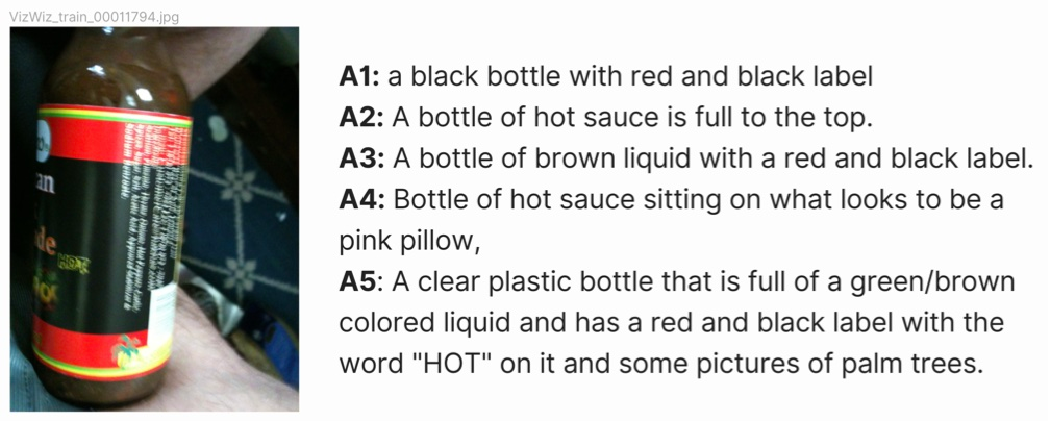
\includegraphics[width=0.5\textwidth]{pics/viswiz.pdf}}
\end{center}

The key parts of the projects include:

\begin{itemize}
\item \textbf{VizWiz} \citep{Gurari2020CaptioningIT}: the dataset of images taken by people who are either blind or visually impared
\pause
\item \textbf{Image Captioning model with Attention} \citep{xu2015}
\pause
\item Evaluation: report \textbf{accuracy, loss, NLG evaluation metrics} (e.g., BLEU \citep{papineni2002}), analyse attention on the image

\end{itemize}

\end{frame}




\begin{frame}

\frametitle{Basics of Sequence Networks\footnote{\url{http://karpathy.github.io/2015/05/21/rnn-effectiveness/}}}

\begin{center}
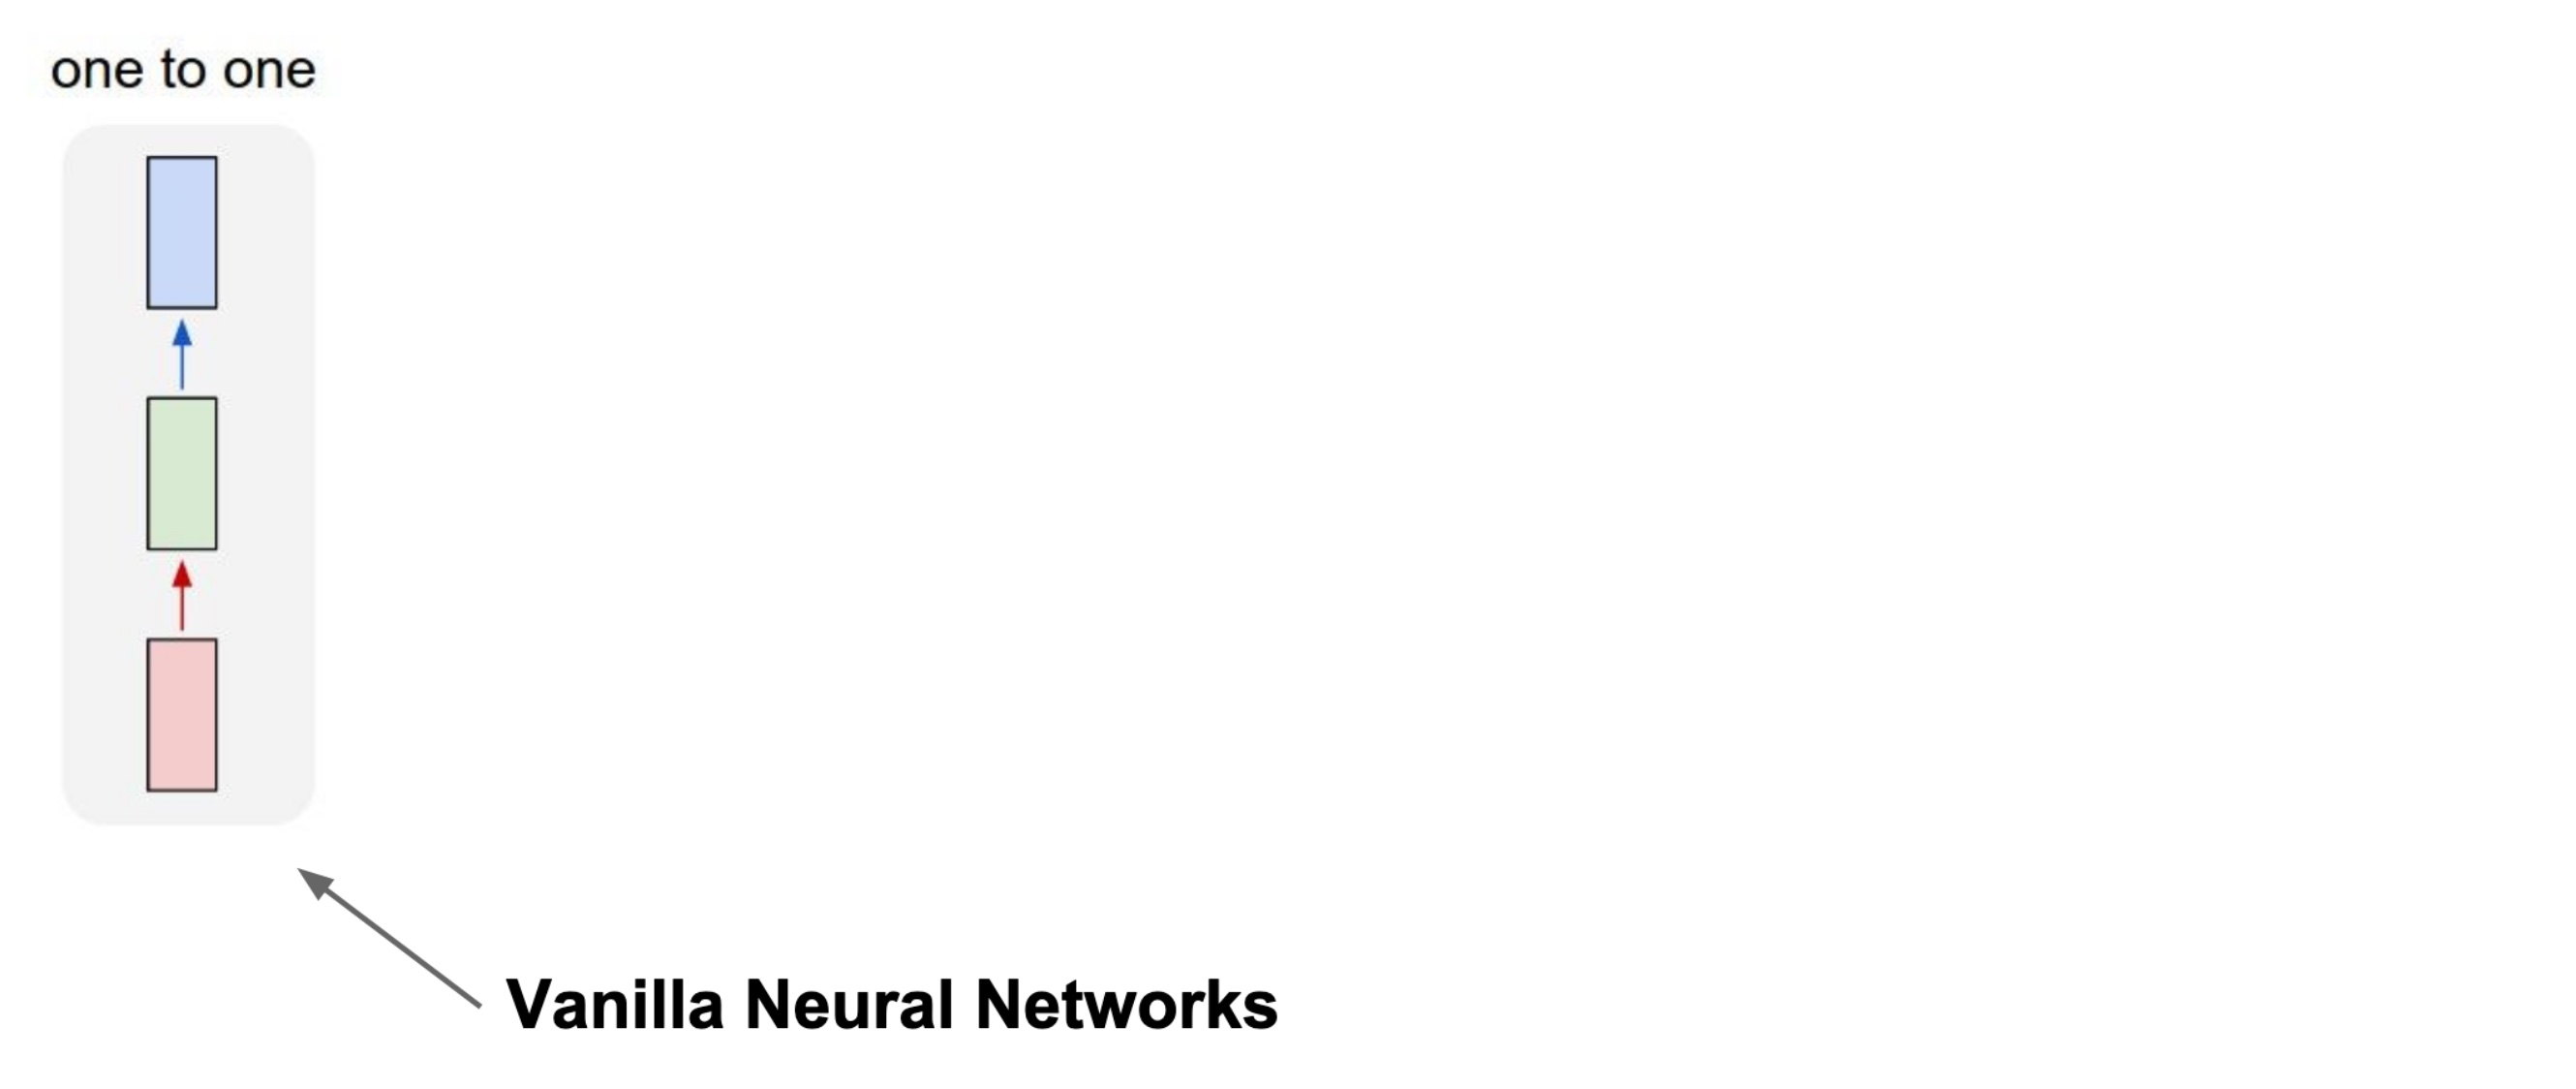
\includegraphics[width=\textwidth]{pics/vanillarnn}
\end{center}

\end{frame}



\begin{frame}

\frametitle{Basics of Sequence Networks}

\begin{center}
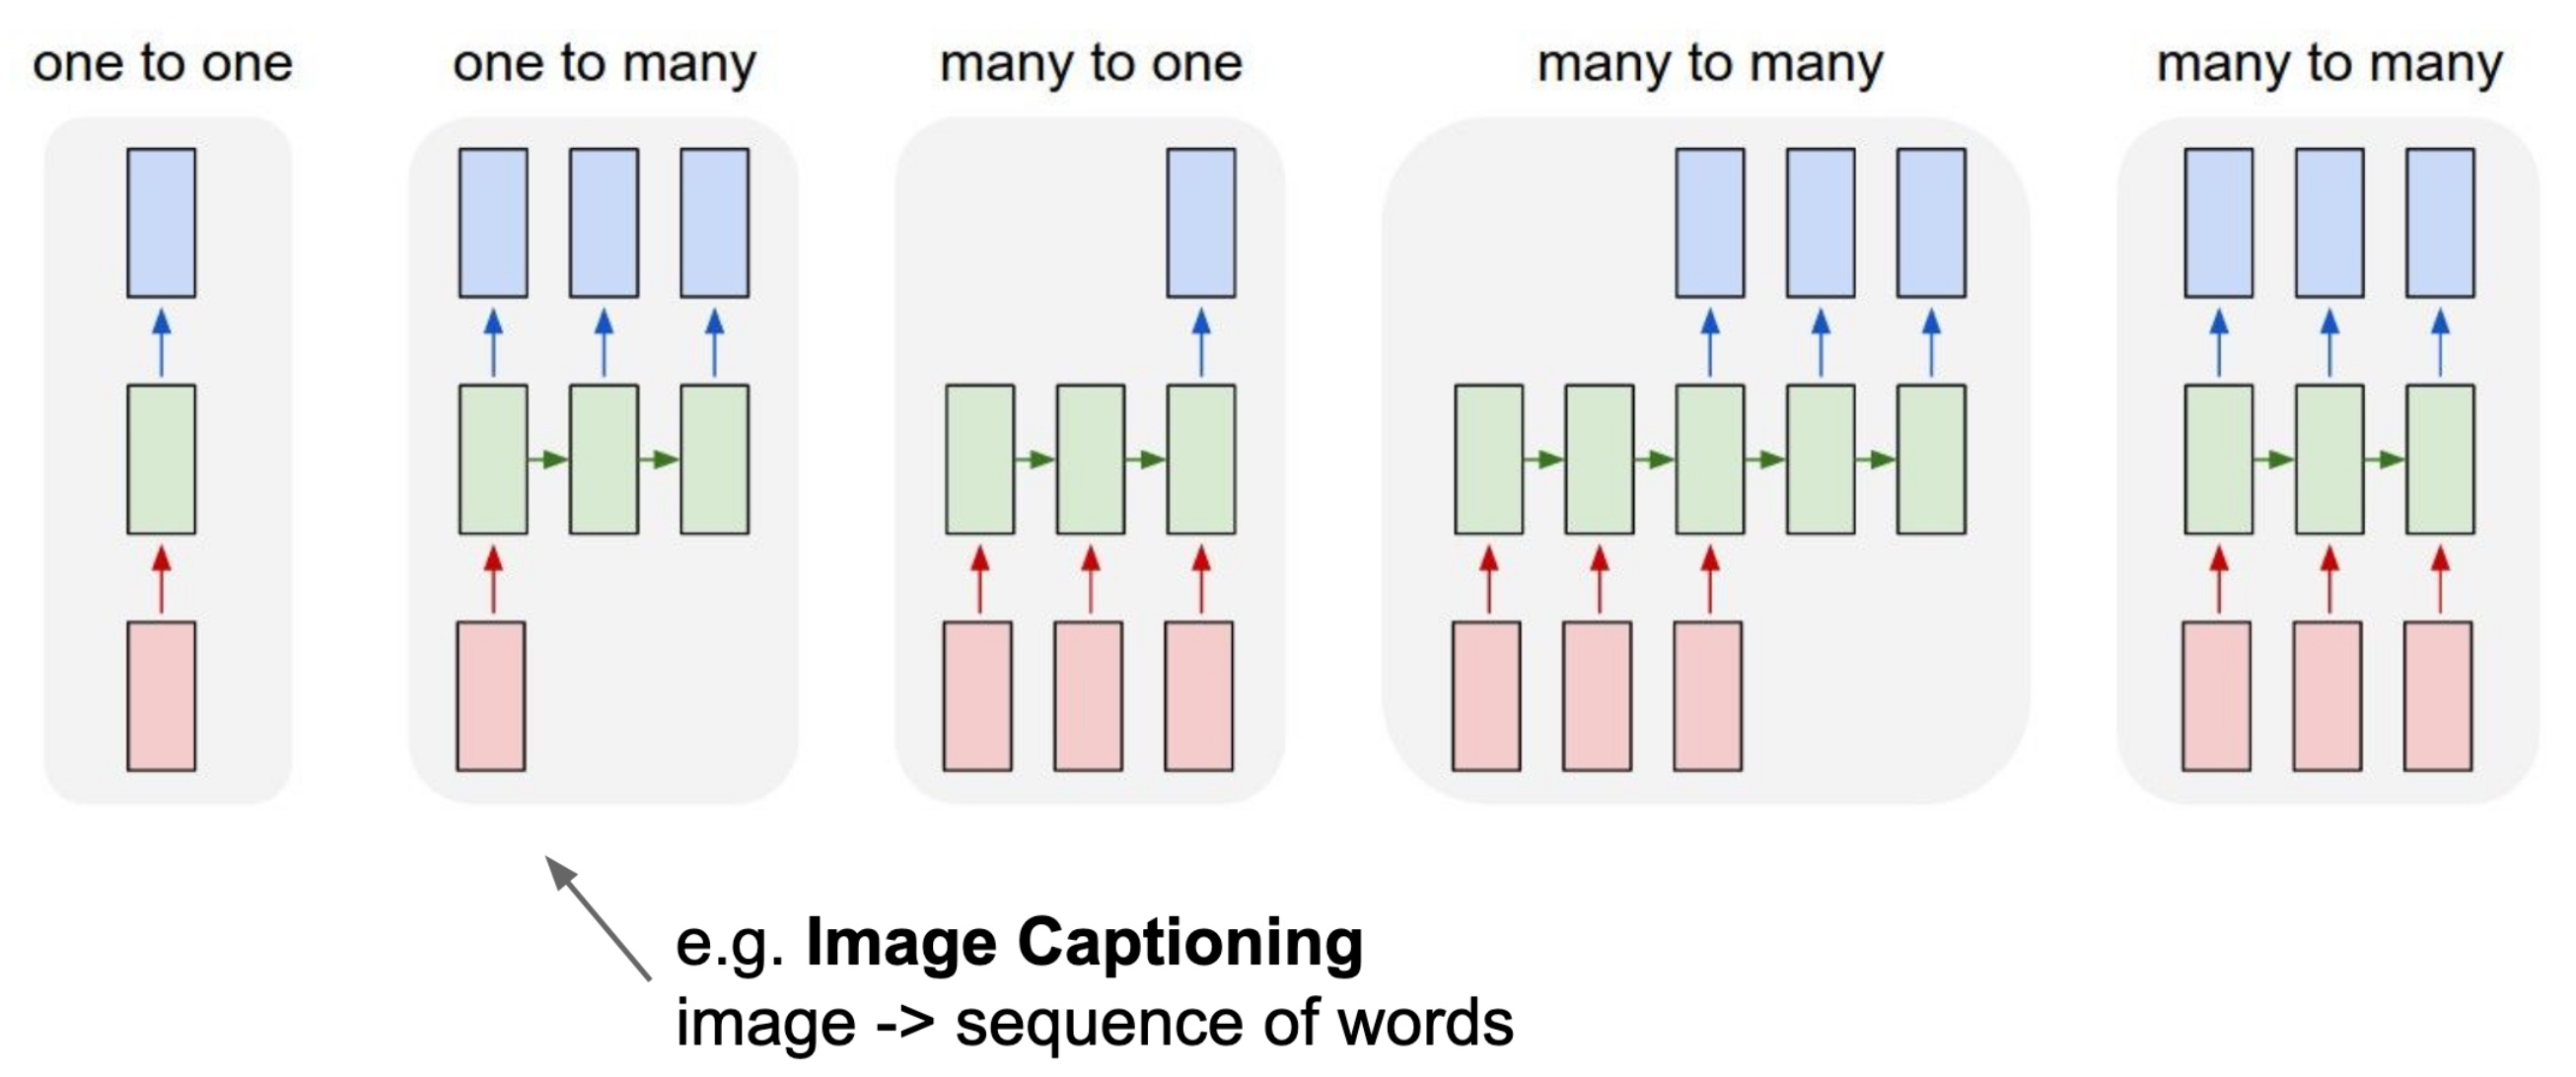
\includegraphics[width=\textwidth]{pics/rnn2}
\end{center}

\end{frame}


\begin{frame}

\frametitle{Basics of Sequence Networks}

\begin{center}
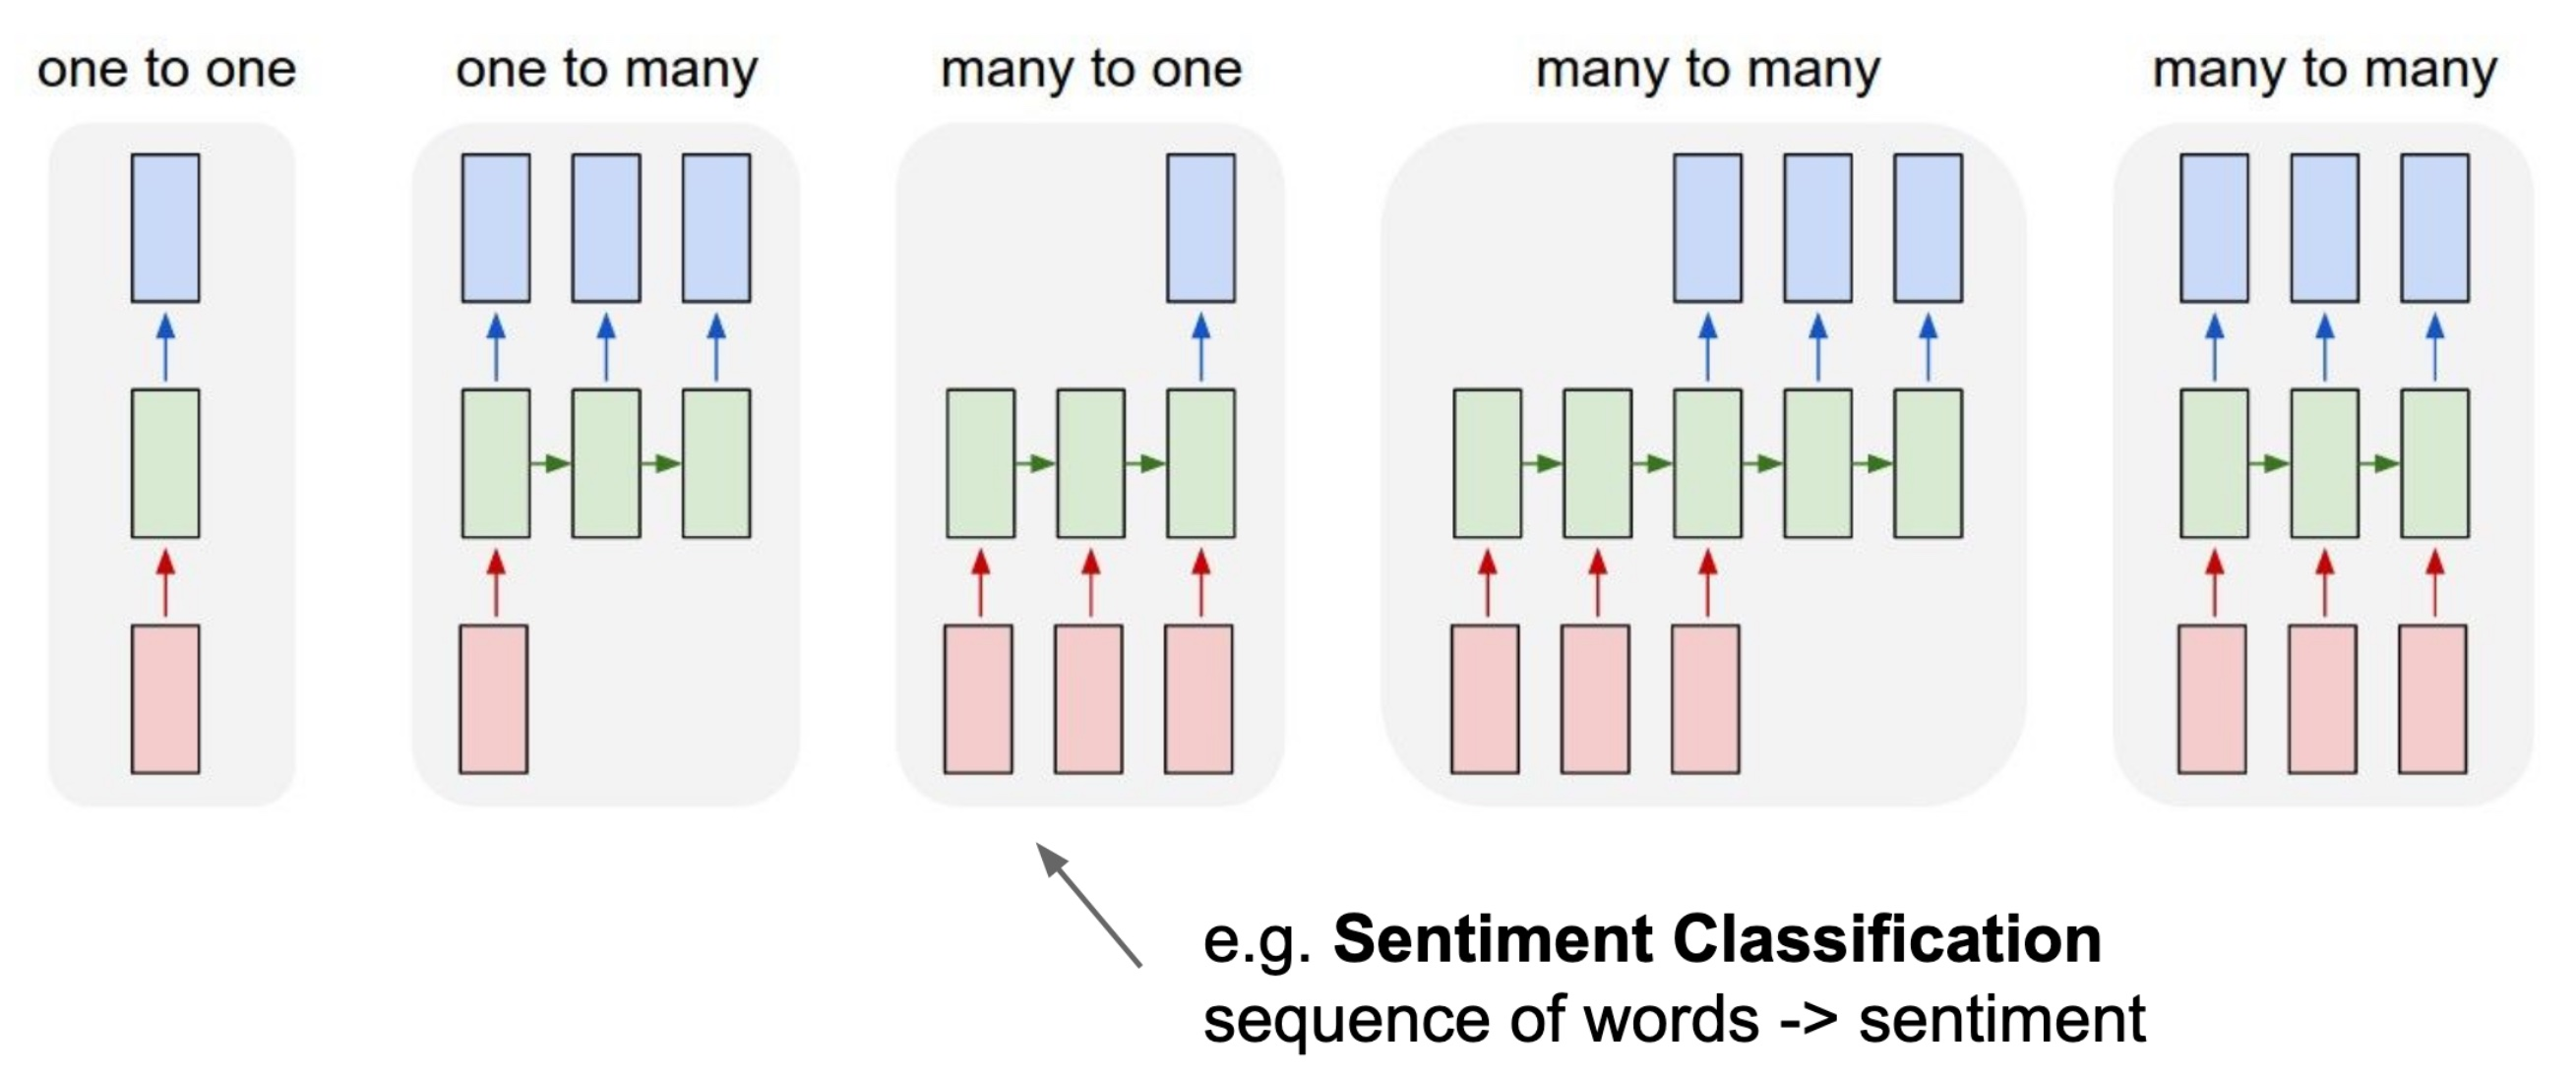
\includegraphics[width=\textwidth]{pics/rnn3}
\end{center}

\end{frame}



\begin{frame}

\frametitle{Basics of Sequence Networks}

\begin{center}
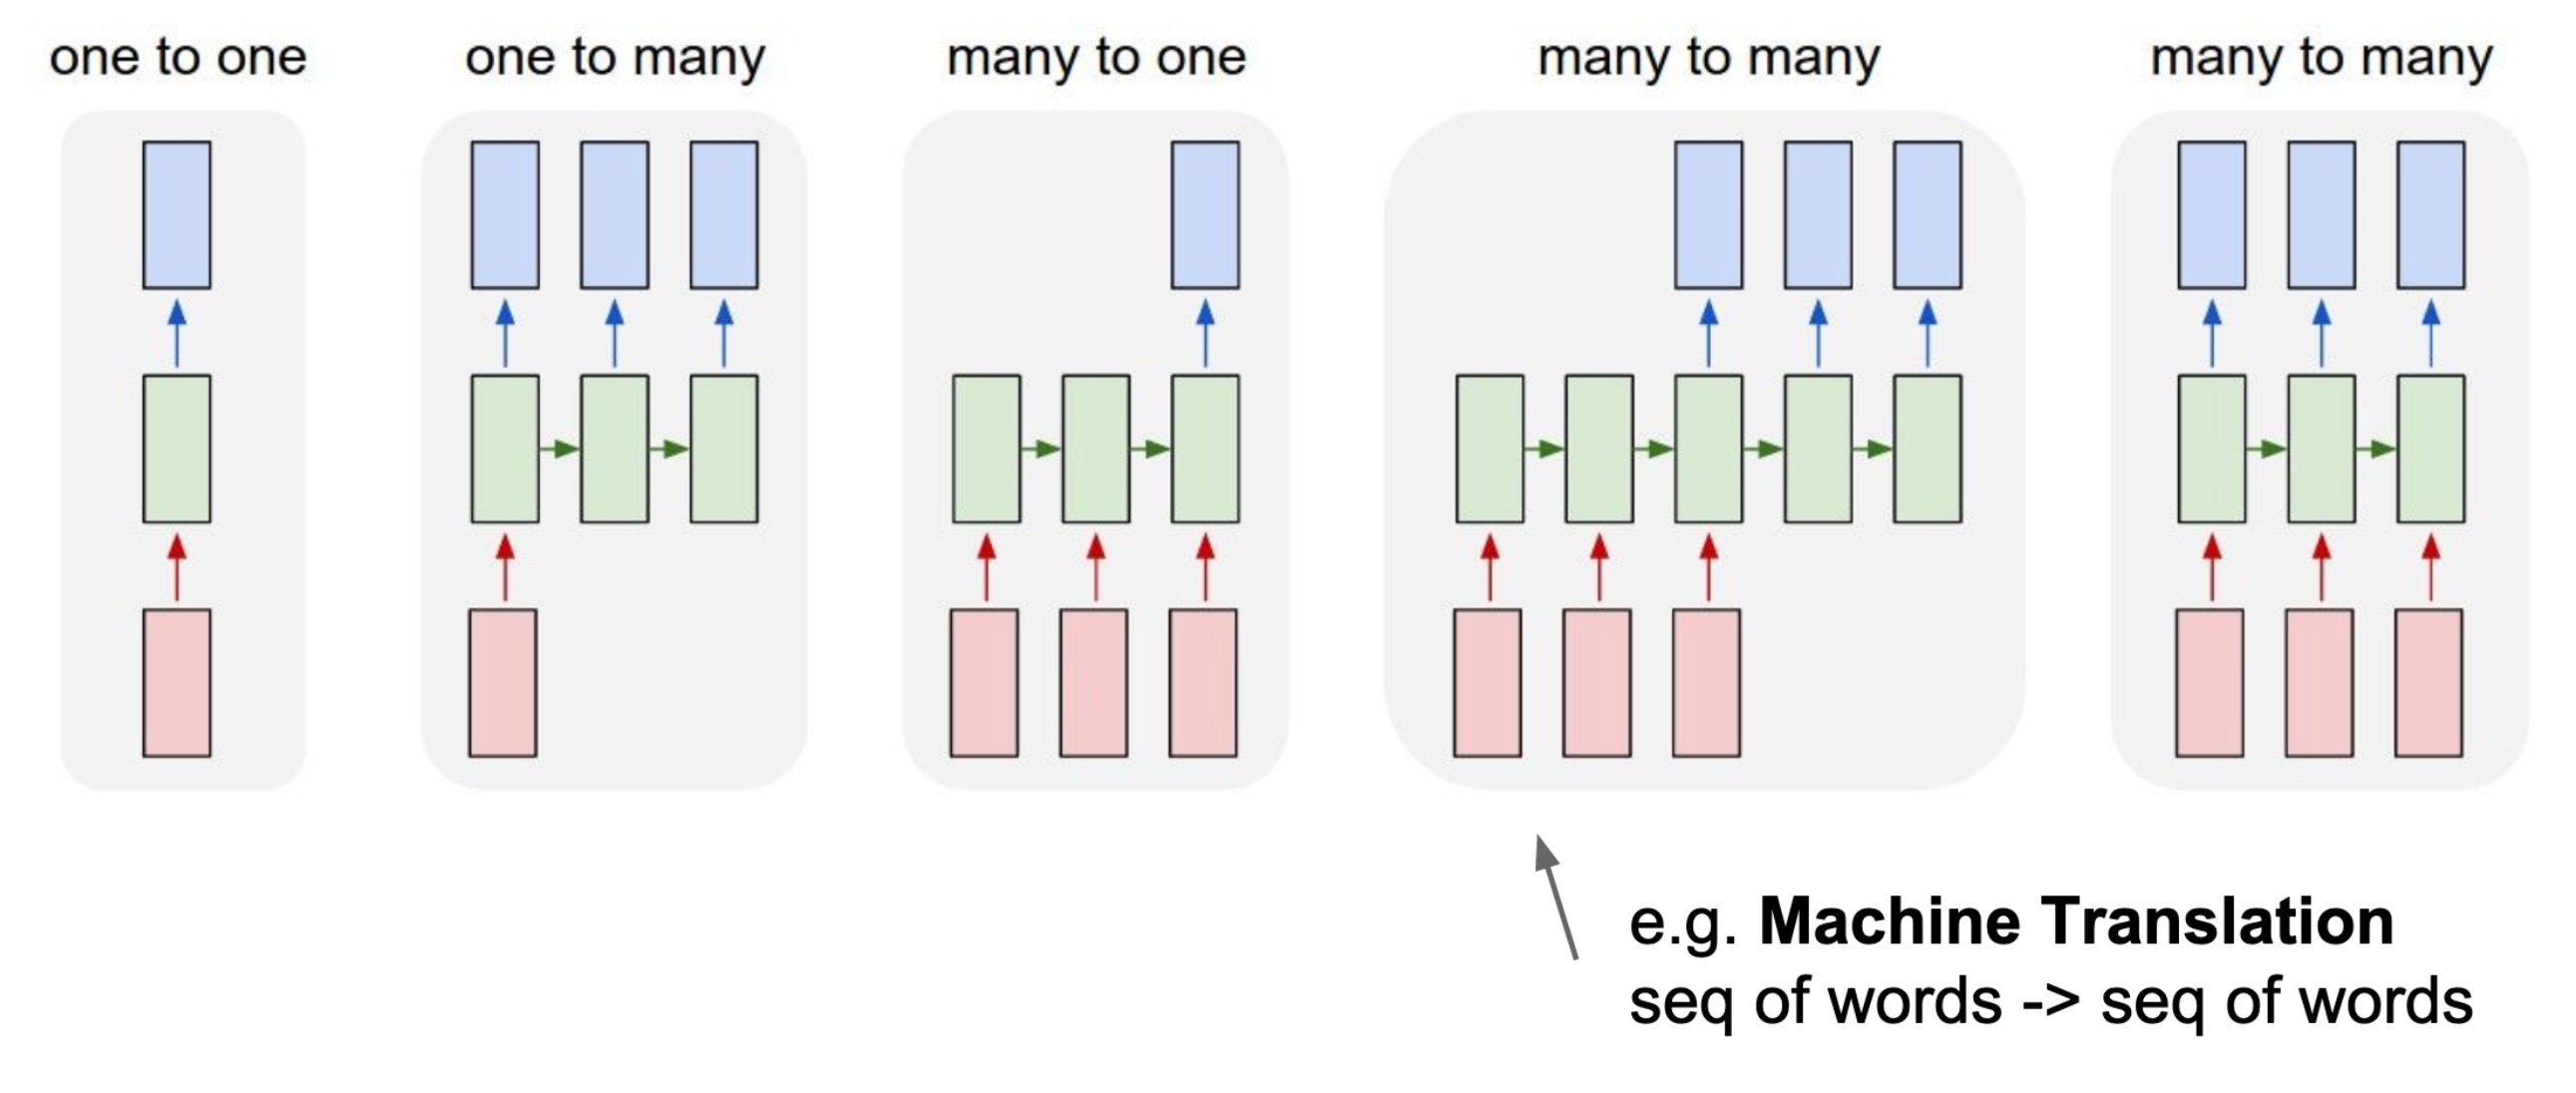
\includegraphics[width=\textwidth]{pics/rnn4}
\end{center}

\end{frame}



\begin{frame}

\frametitle{Basics of Sequence Networks}

\begin{center}
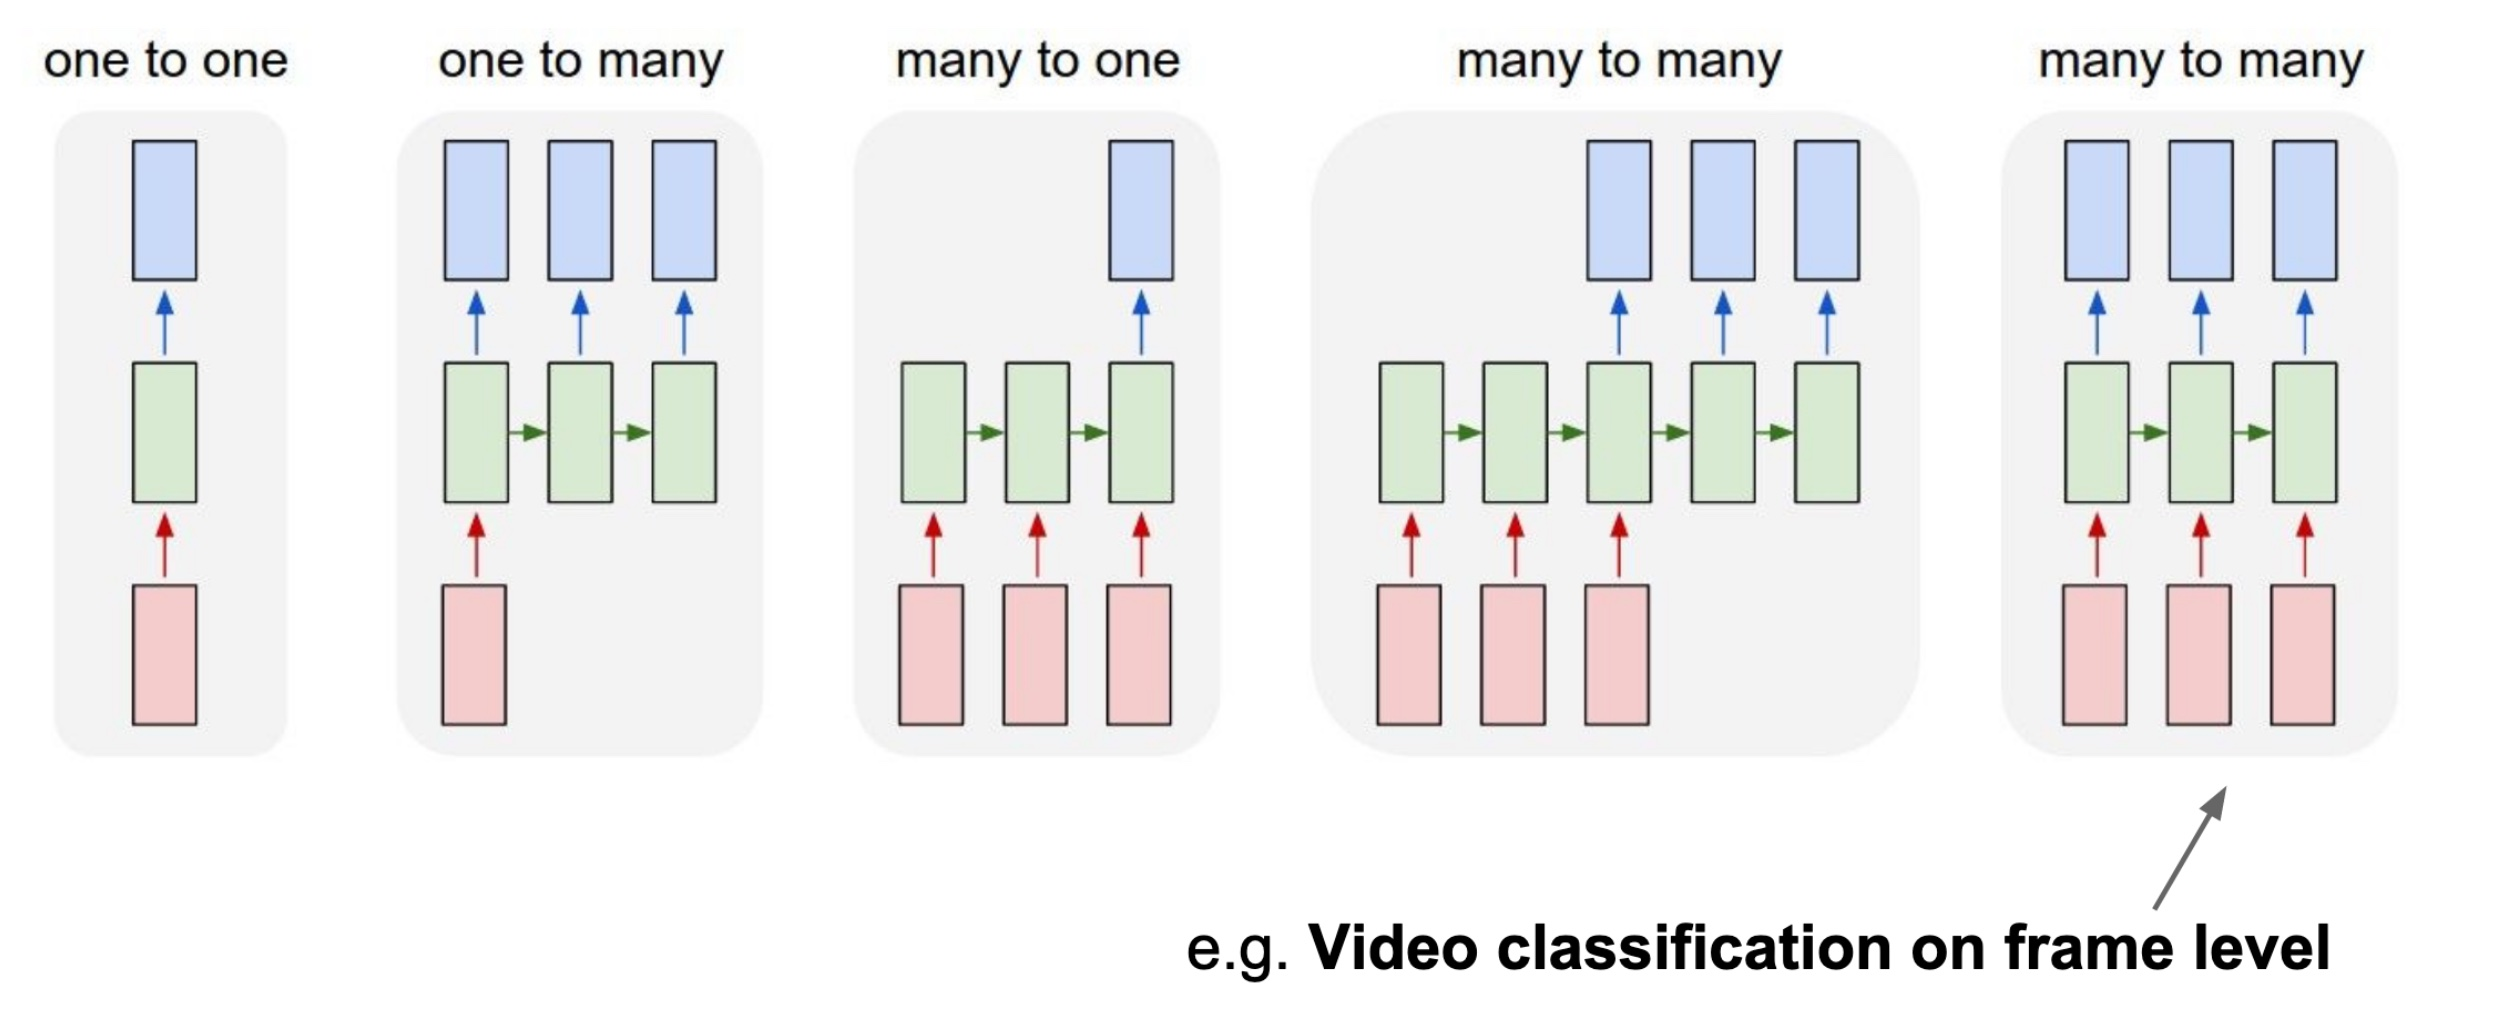
\includegraphics[width=\textwidth]{pics/rnn5}
\end{center}

\end{frame}


\begin{frame}

\frametitle{Recurrent Neural Network\footnote{\url{http://cs231n.stanford.edu/slides/2017/cs231n_2017_lecture10.pdf}}}

\begin{center}
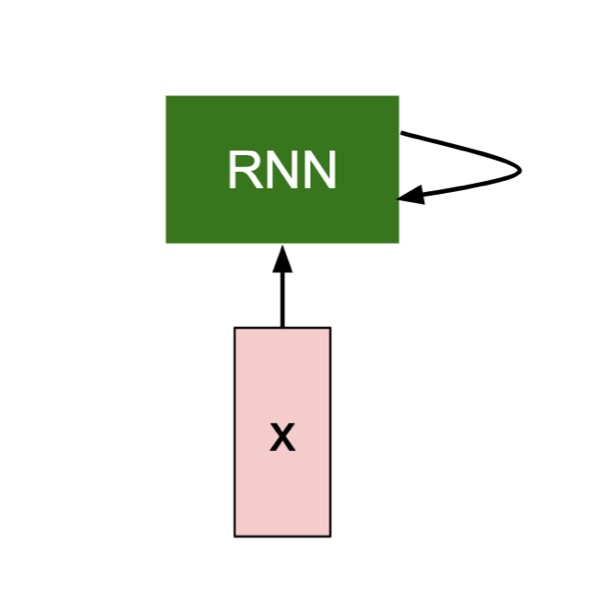
\includegraphics[width=.5\textwidth]{pics/rnnhow1}
\end{center}

\end{frame}


\begin{frame}

\frametitle{Recurrent Neural Network}

\begin{center}
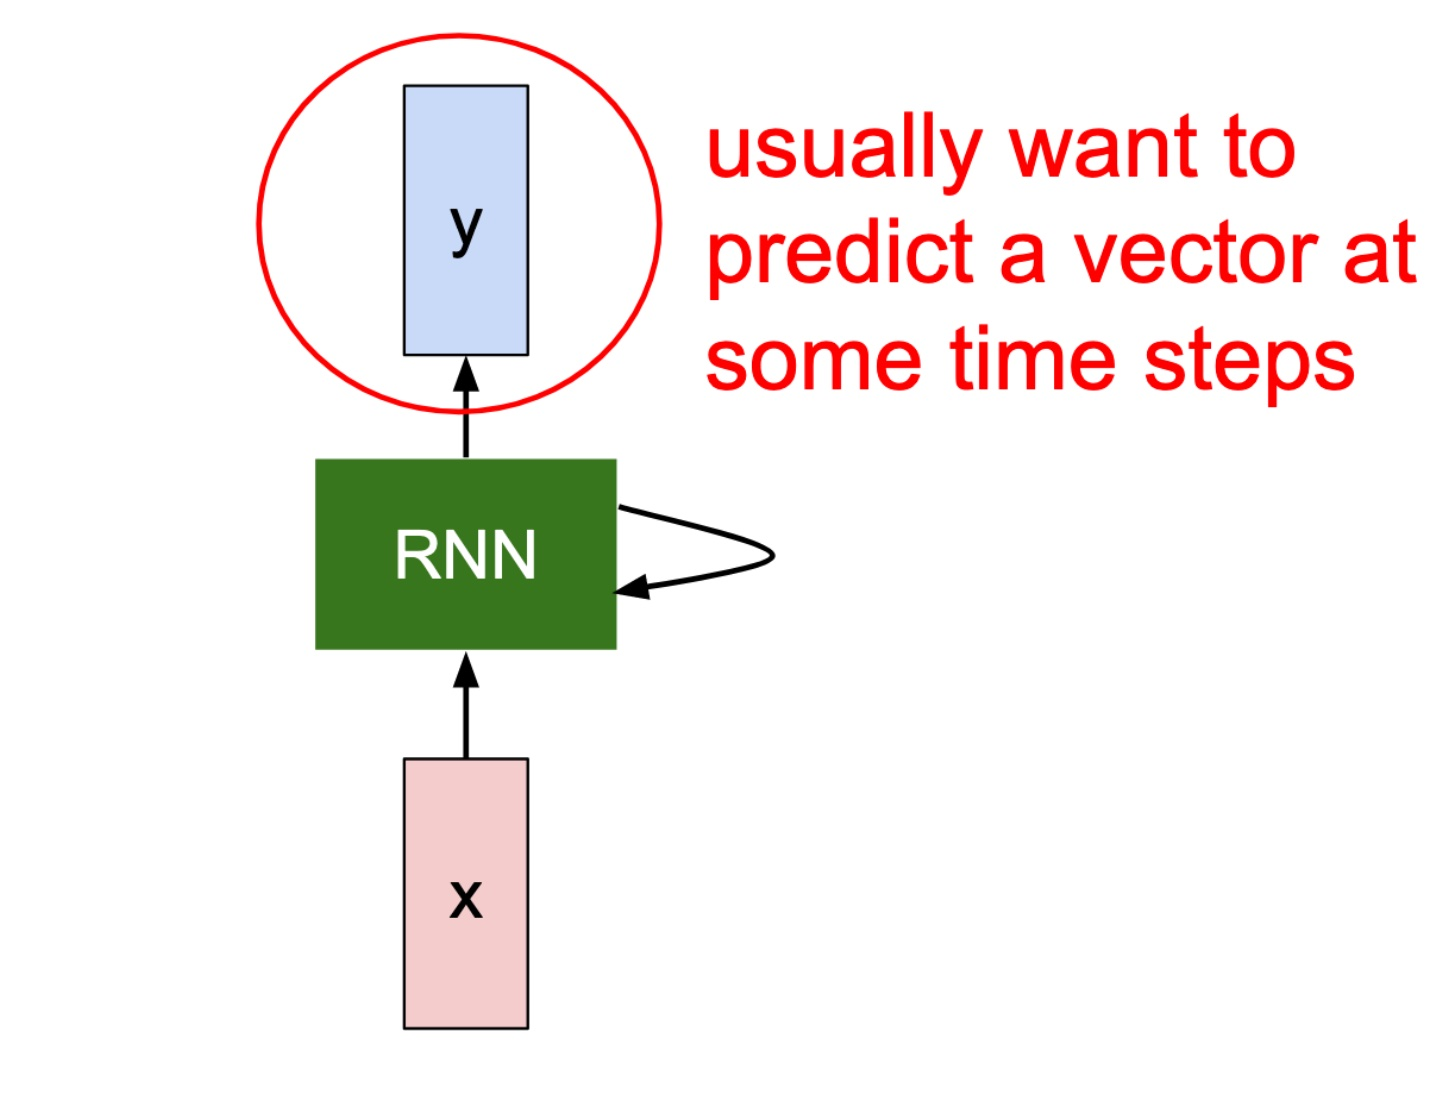
\includegraphics[width=.5\textwidth]{pics/rnnhow2}
\end{center}

\end{frame}


\begin{frame}

\frametitle{Recurrent Neural Network}

\begin{center}
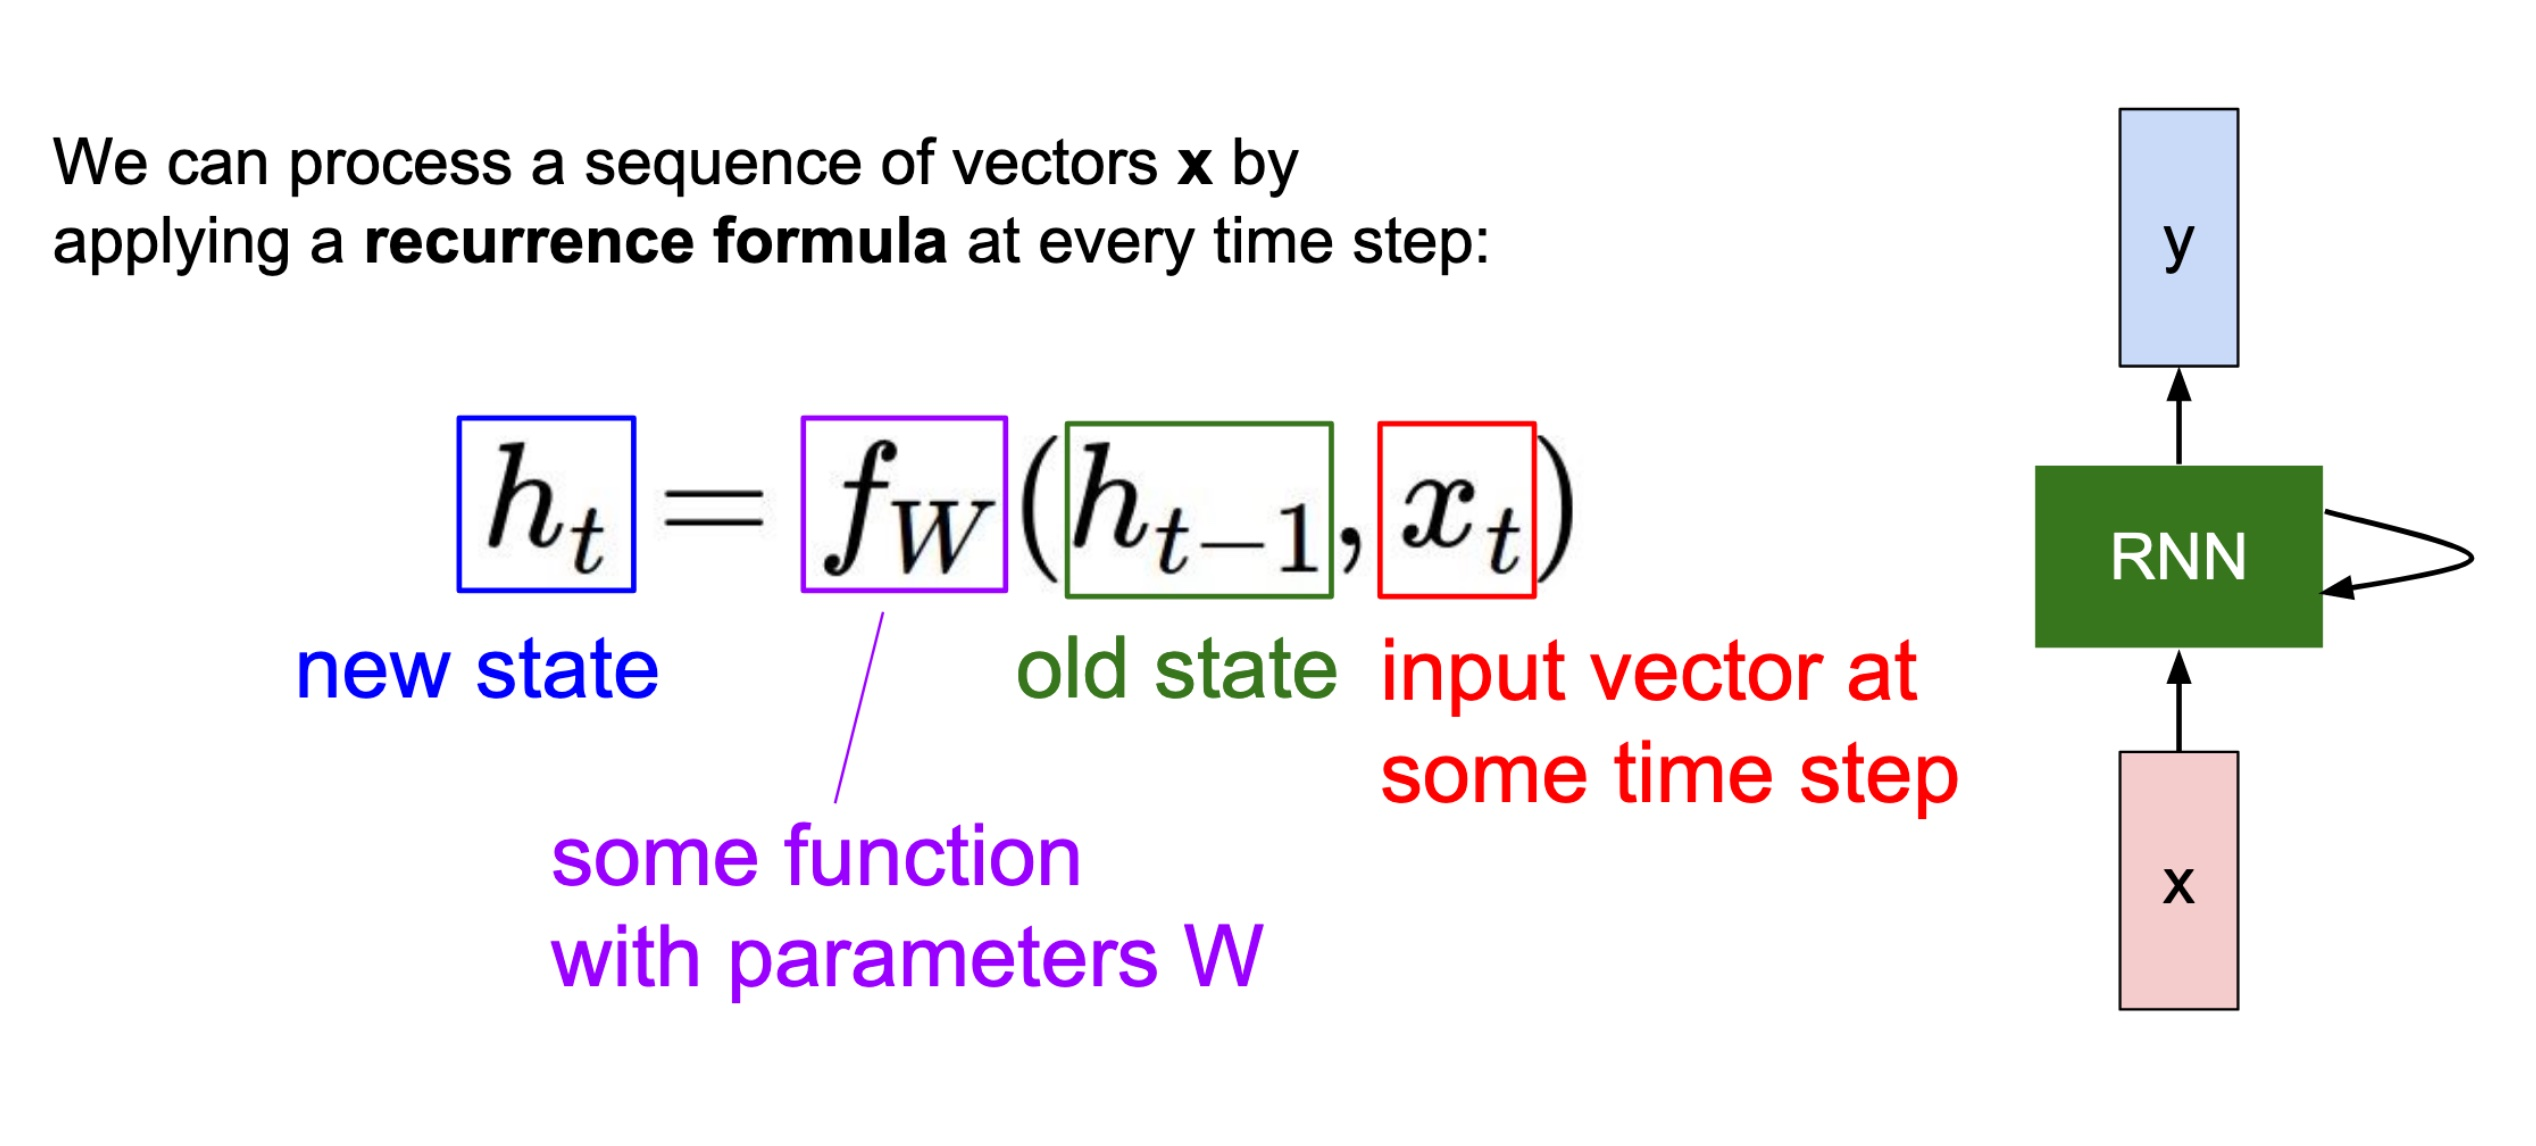
\includegraphics[width=1\textwidth]{pics/rnnhow3}
\end{center}

\end{frame}


\begin{frame}

\frametitle{Recurrent Neural Network}

\begin{center}
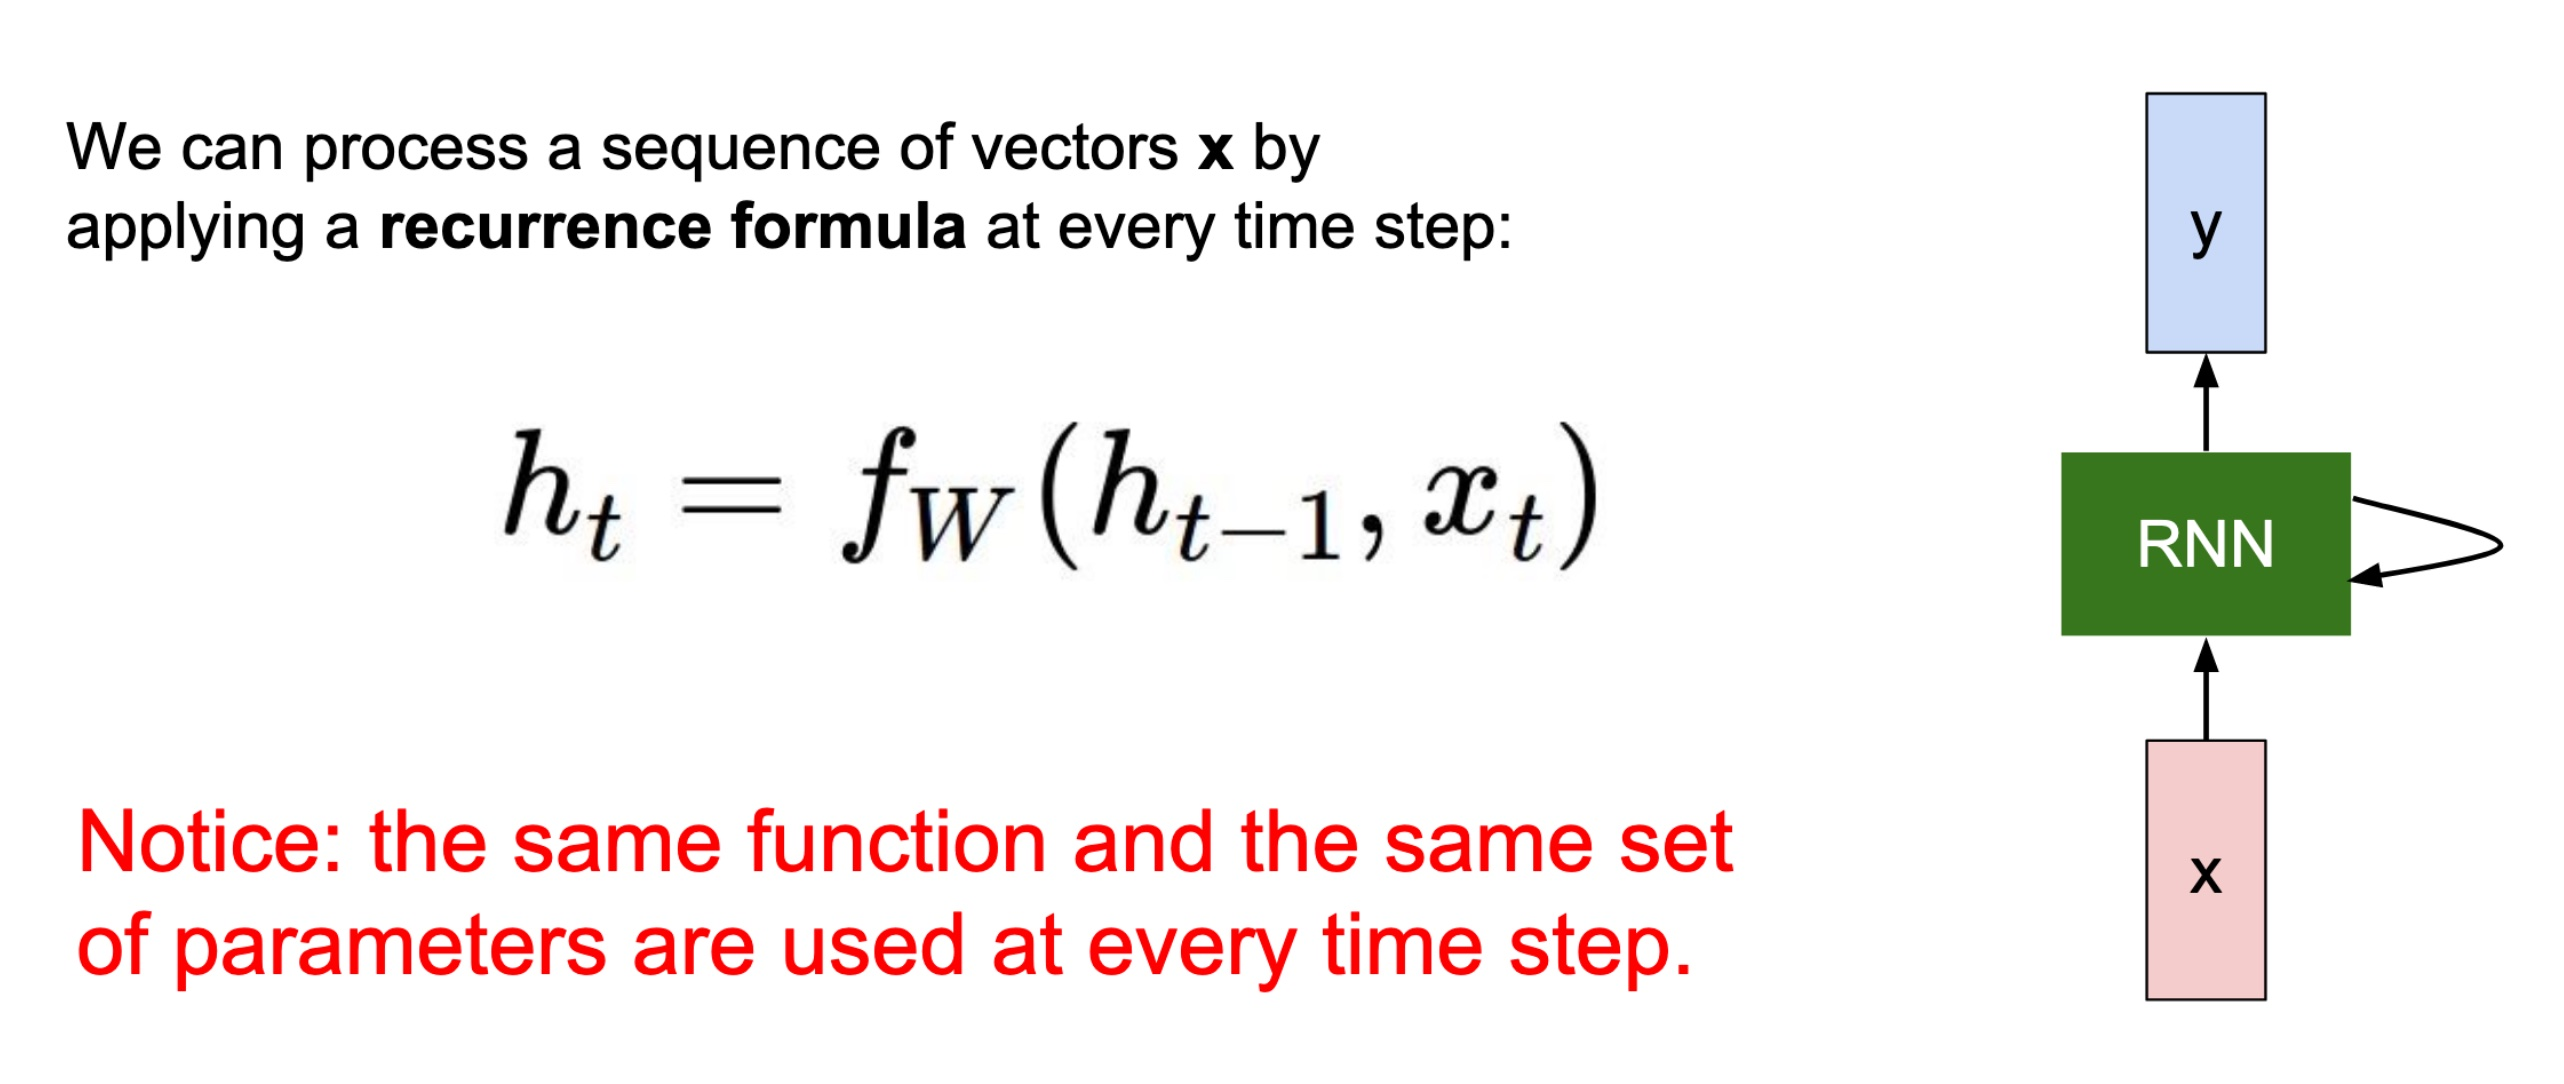
\includegraphics[width=\textwidth]{pics/rnnhow4}
\end{center}

\end{frame}


\begin{frame}

\frametitle{Recurrent Neural Network}

\begin{center}
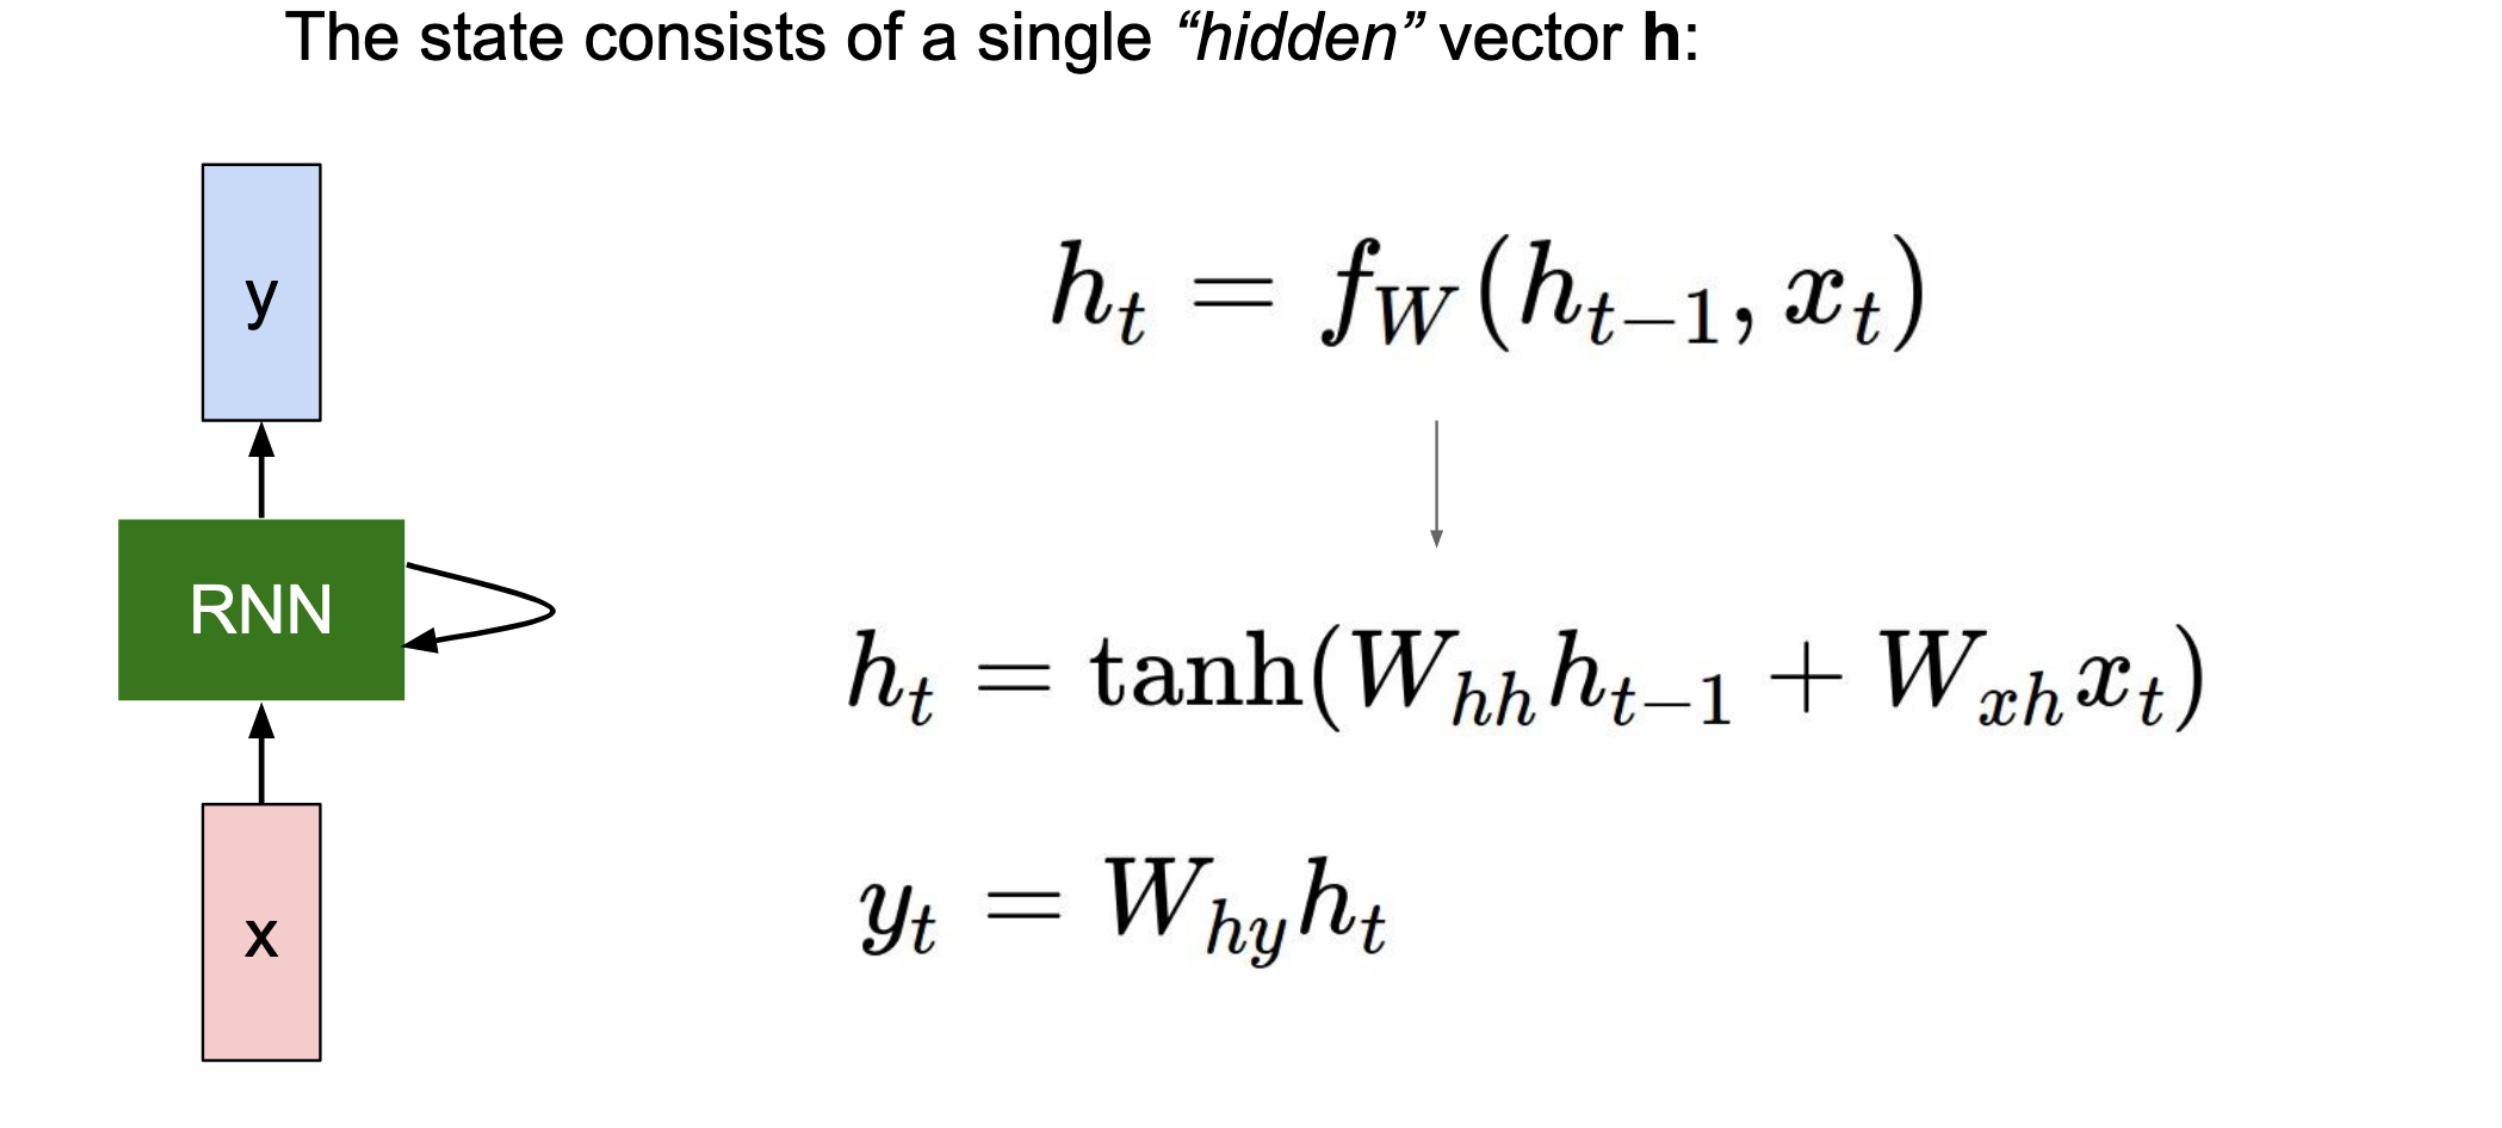
\includegraphics[width=\textwidth]{pics/rnnhow5}
\end{center}

Why non-linearity?\footnote{\url{https://stackoverflow.com/questions/9782071/why-must-a-nonlinear-activation-function-be-used-in-a-backpropagation-neural-net}}

\end{frame}


\begin{frame}

\frametitle{Recurrent Neural Network: Computational Graph}

\begin{center}
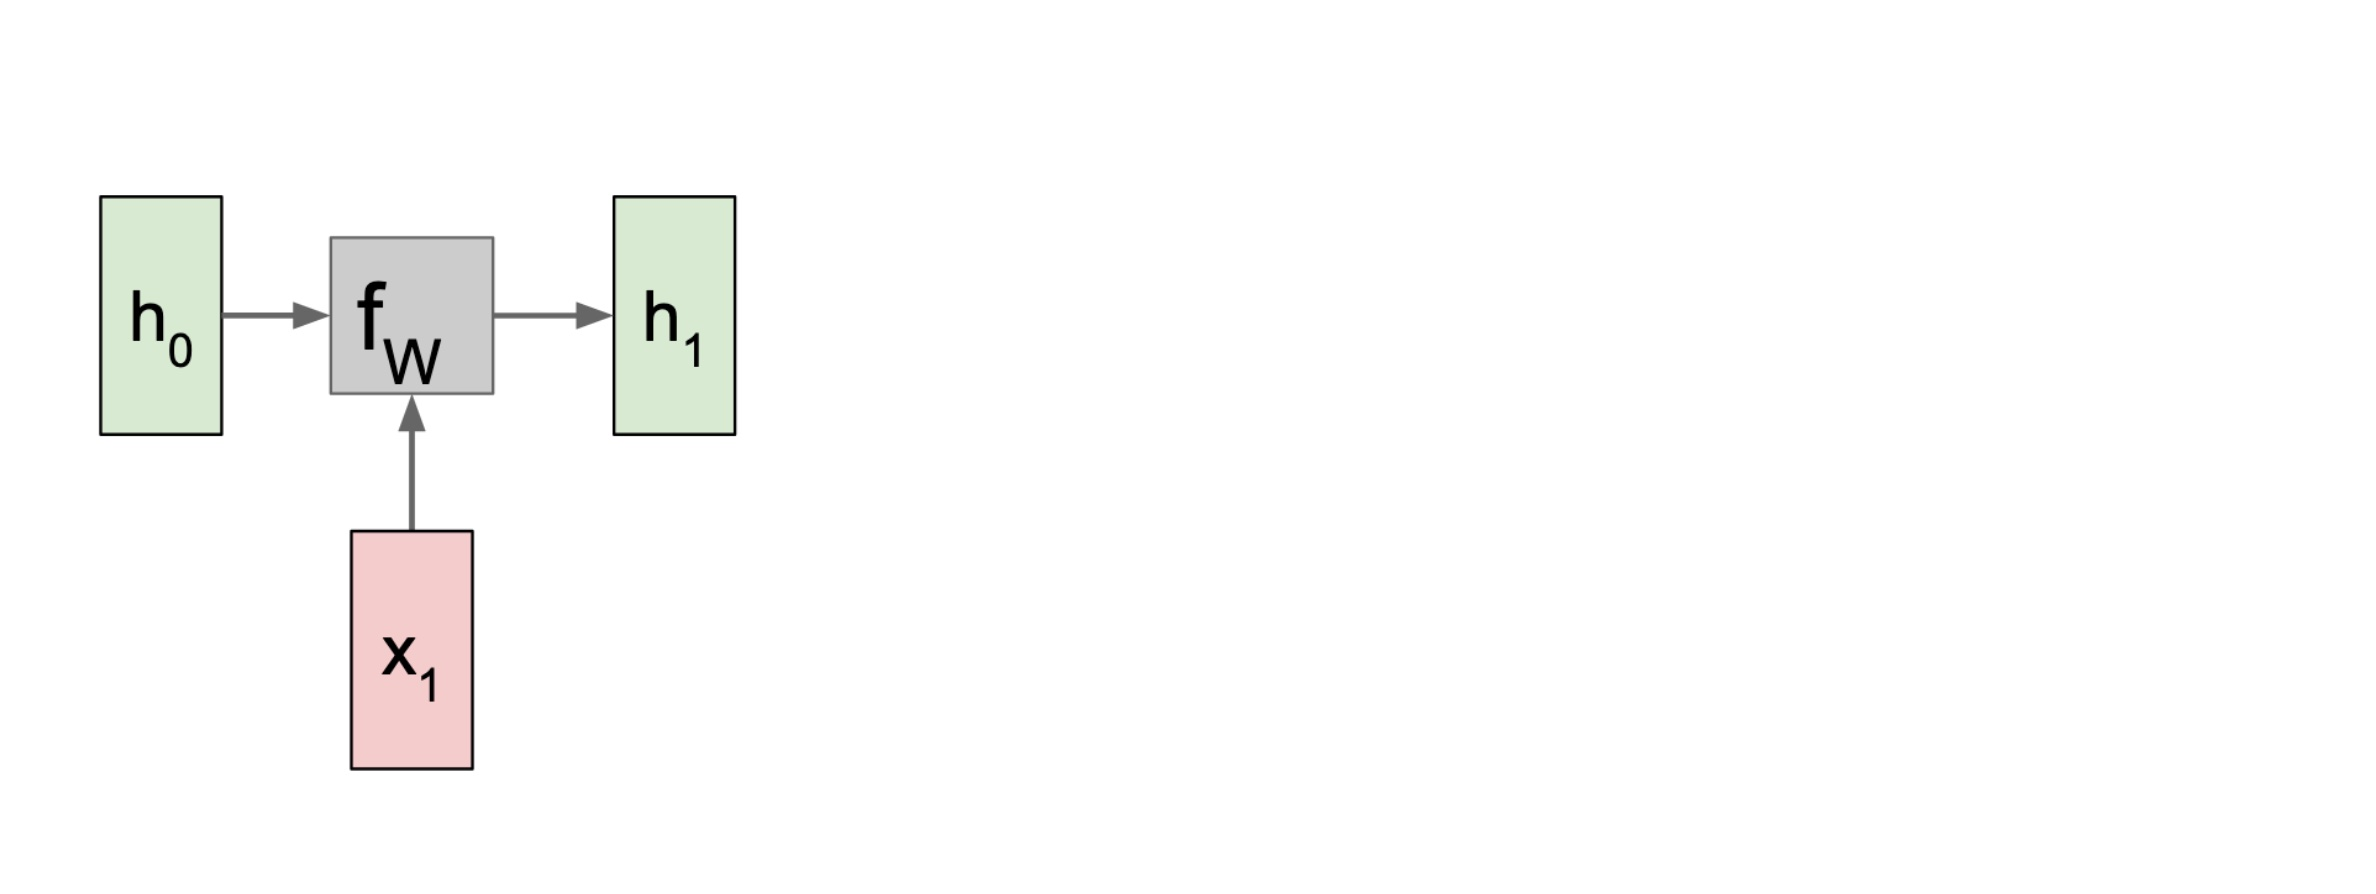
\includegraphics[width=\textwidth]{pics/rnngraph1}
\end{center}

\end{frame}

\begin{frame}

\frametitle{Recurrent Neural Network: Computational Graph}

\begin{center}
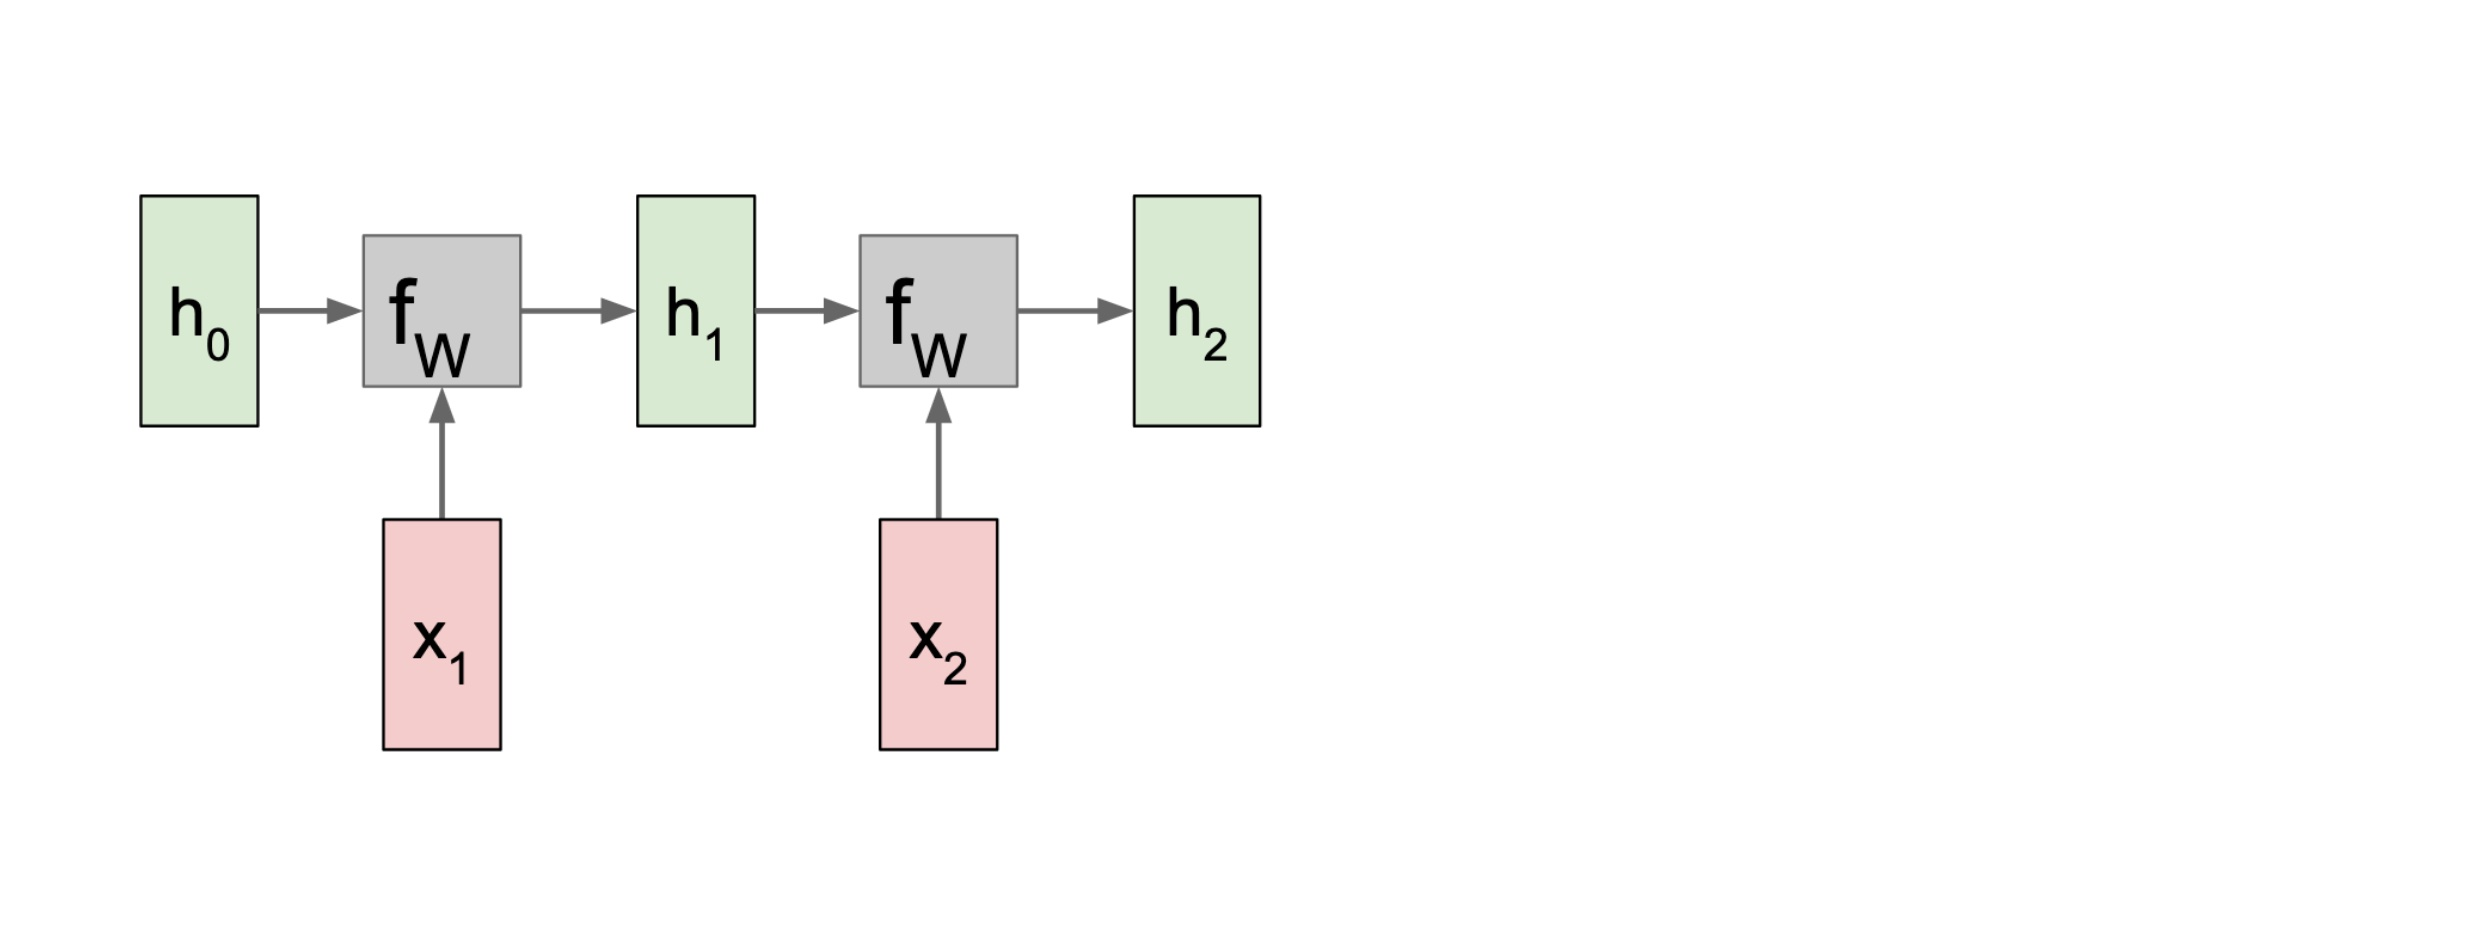
\includegraphics[width=\textwidth]{pics/rnngraph2}
\end{center}

\end{frame}

\begin{frame}

\frametitle{Recurrent Neural Network: Computational Graph}

\begin{center}
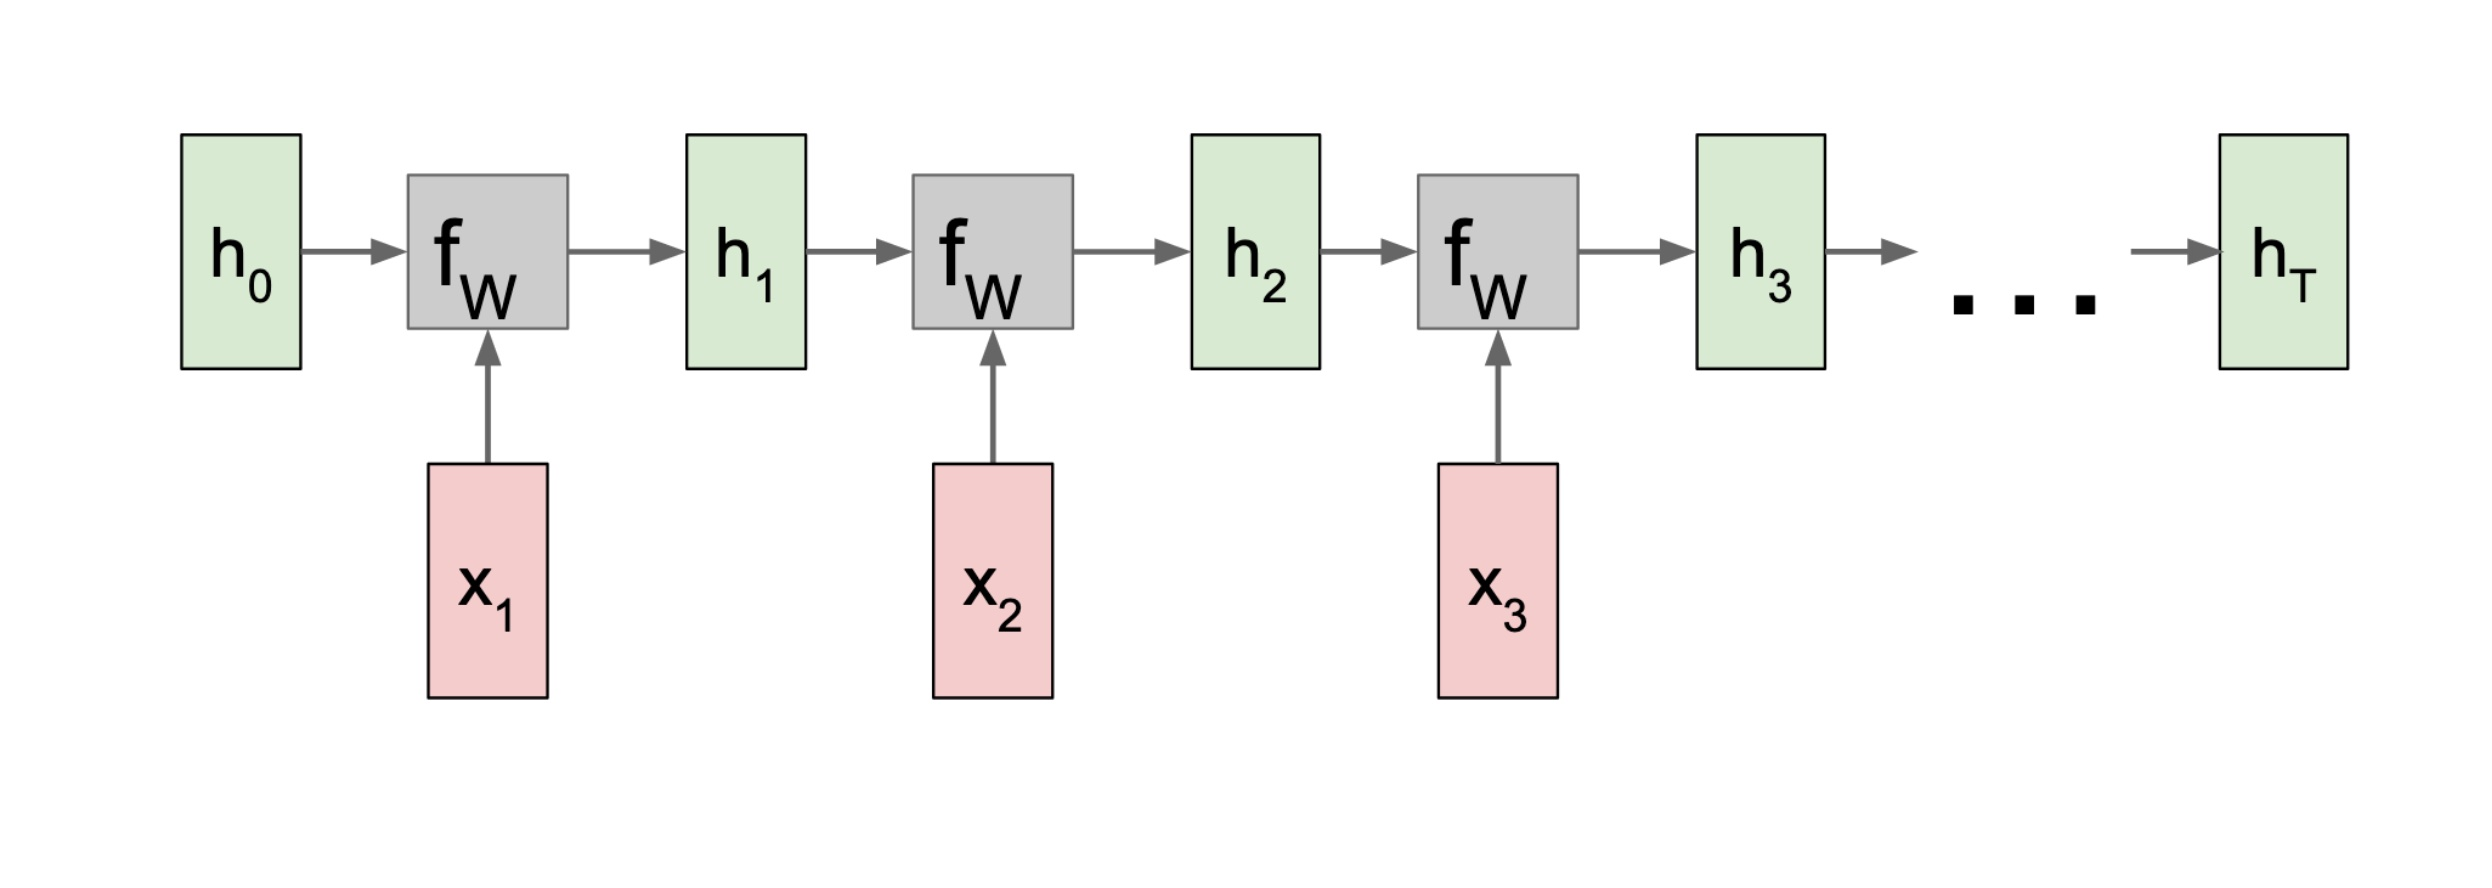
\includegraphics[width=\textwidth]{pics/rnngraph3}
\end{center}

\end{frame}

\begin{frame}

\frametitle{Recurrent Neural Network: Computational Graph}

\begin{center}
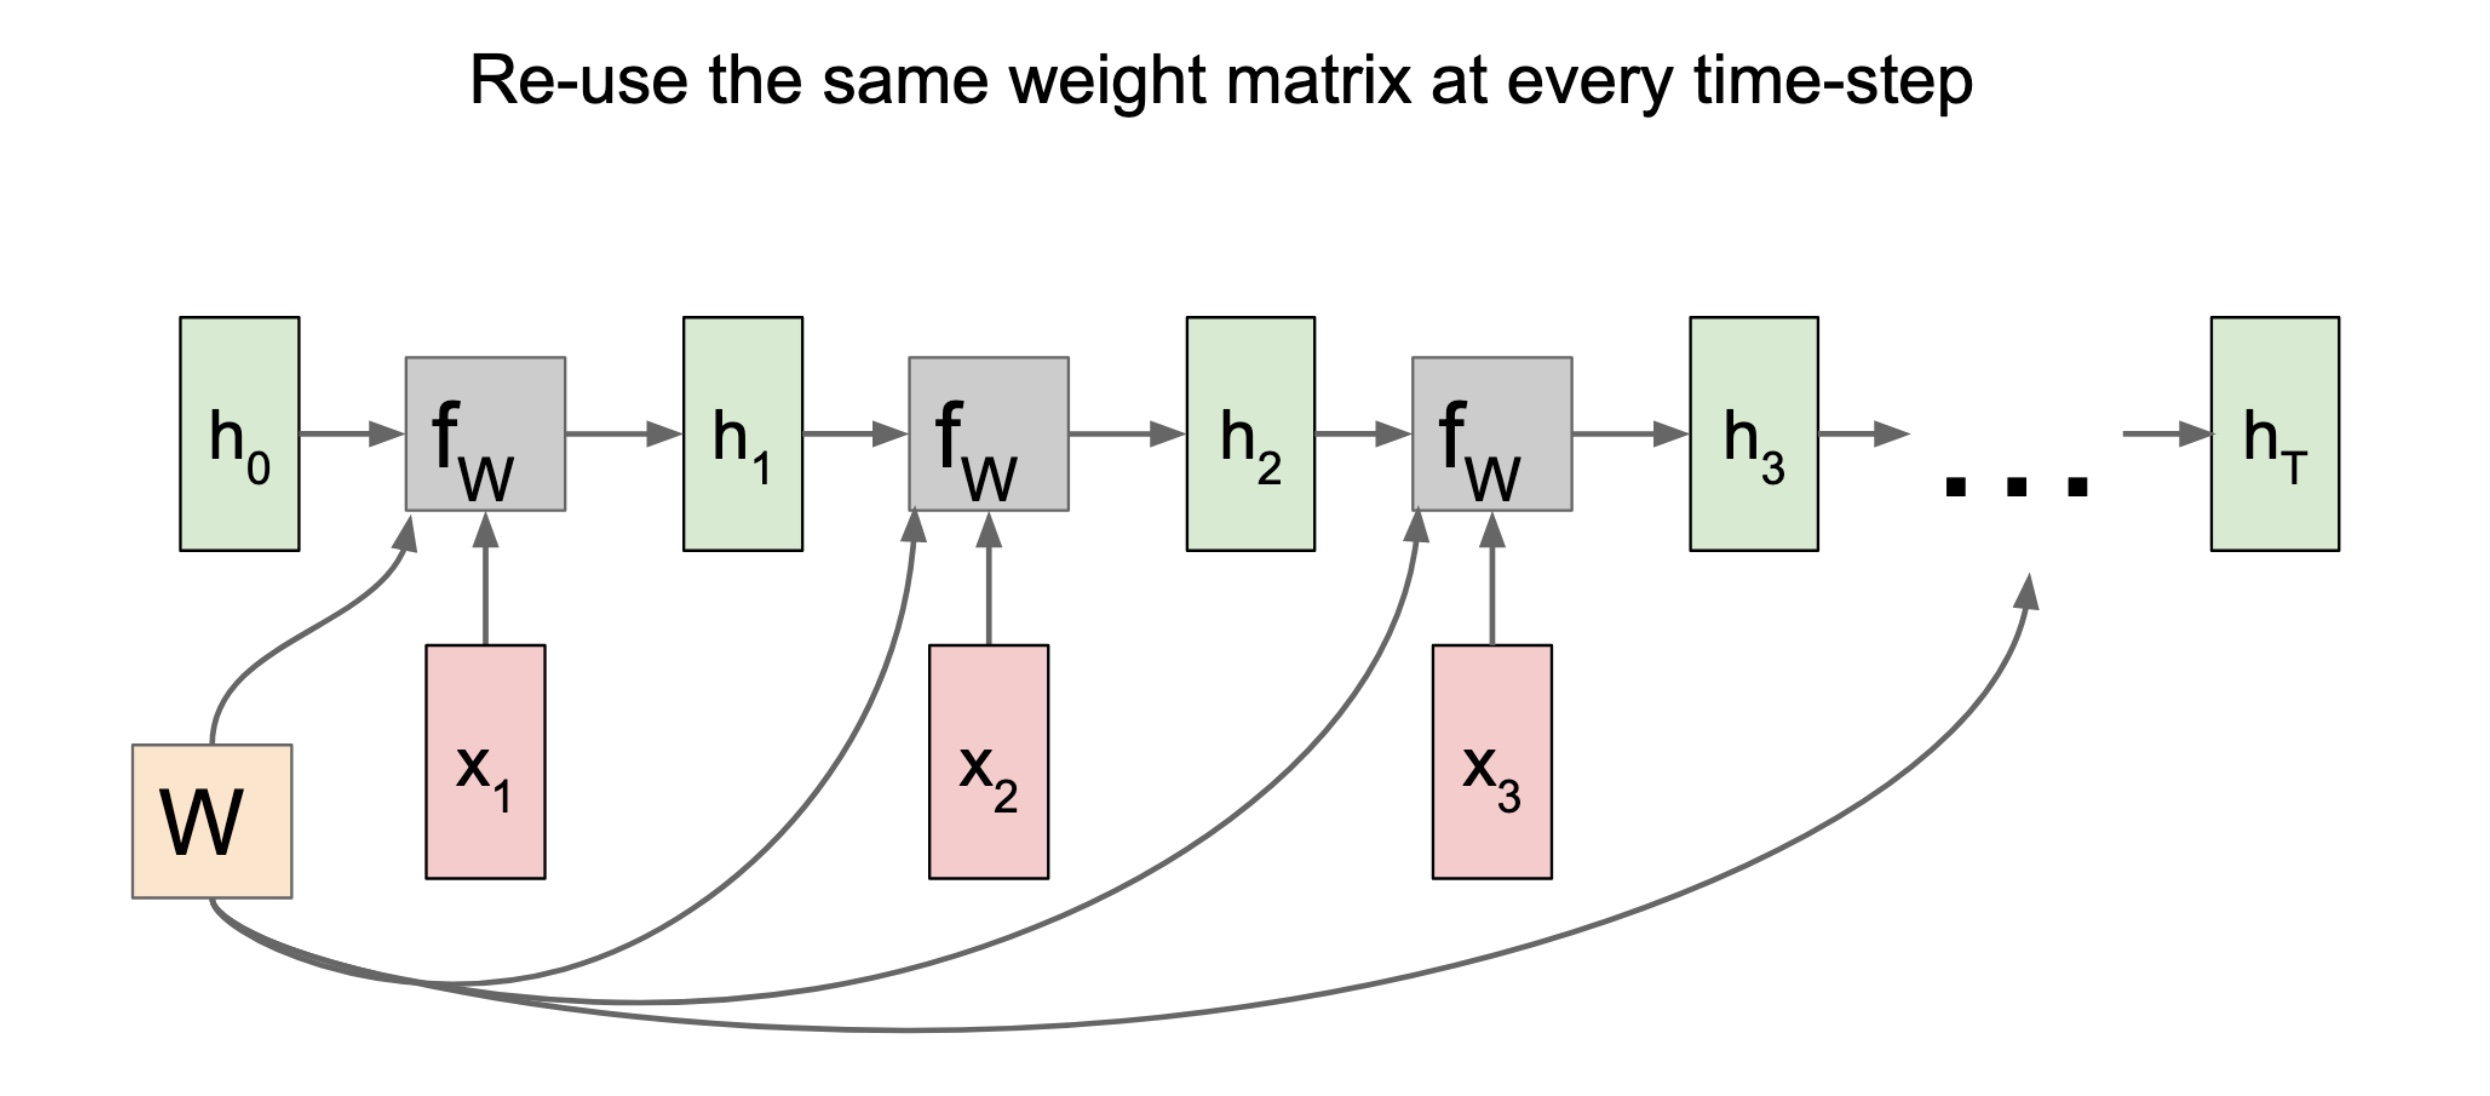
\includegraphics[width=\textwidth]{pics/rnngraph4}
\end{center}

\end{frame}

\begin{frame}

\frametitle{Recurrent Neural Network: Computational Graph}

\begin{center}
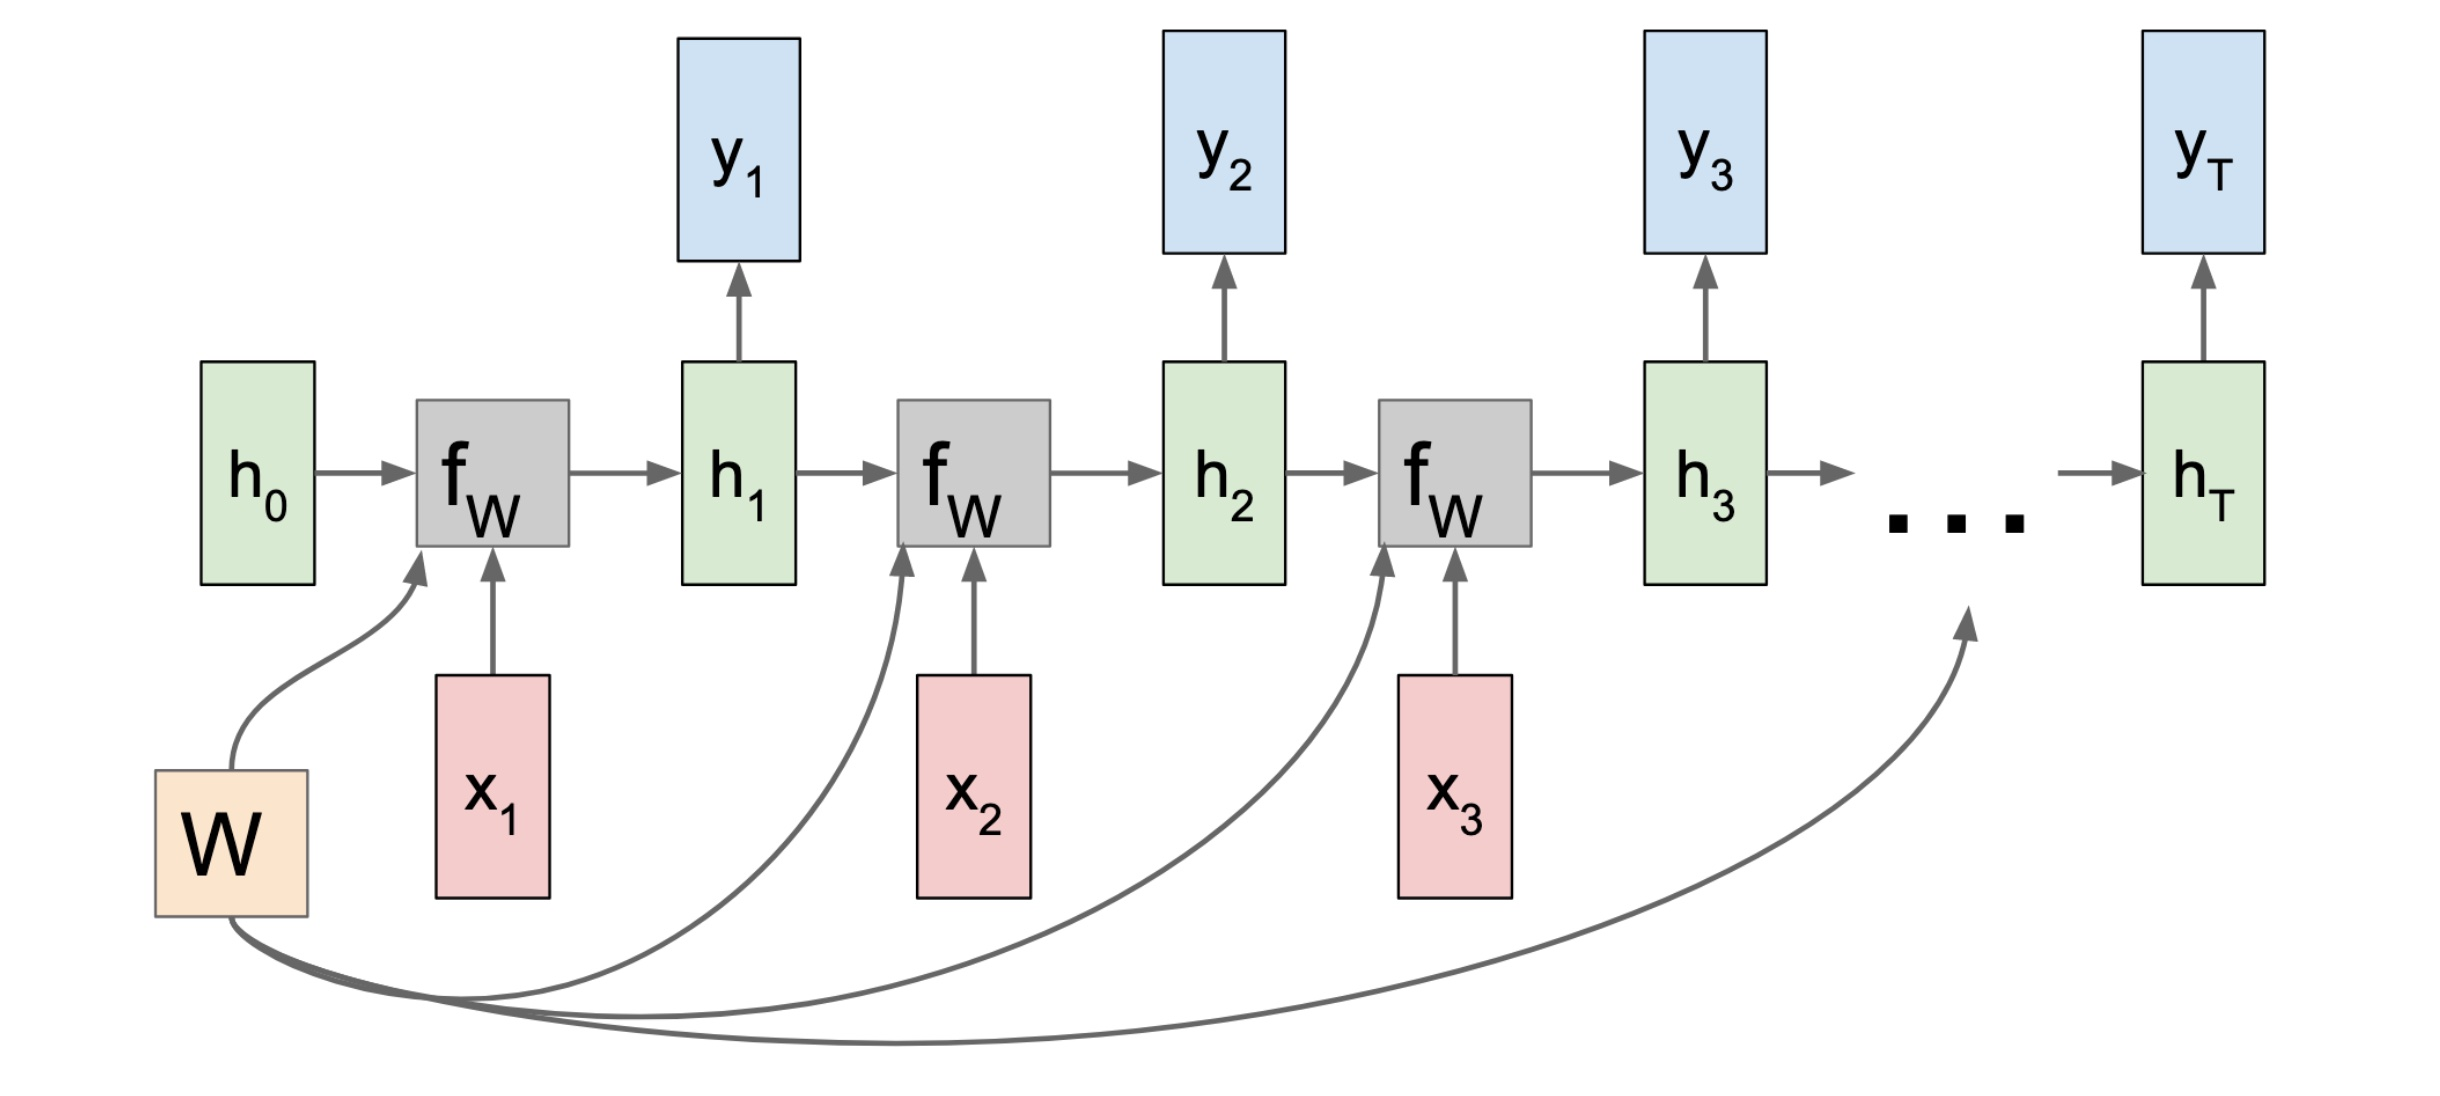
\includegraphics[width=\textwidth]{pics/rnngraph5}
\end{center}

\end{frame}

\begin{frame}

\frametitle{Recurrent Neural Network: Computational Graph}

\begin{center}
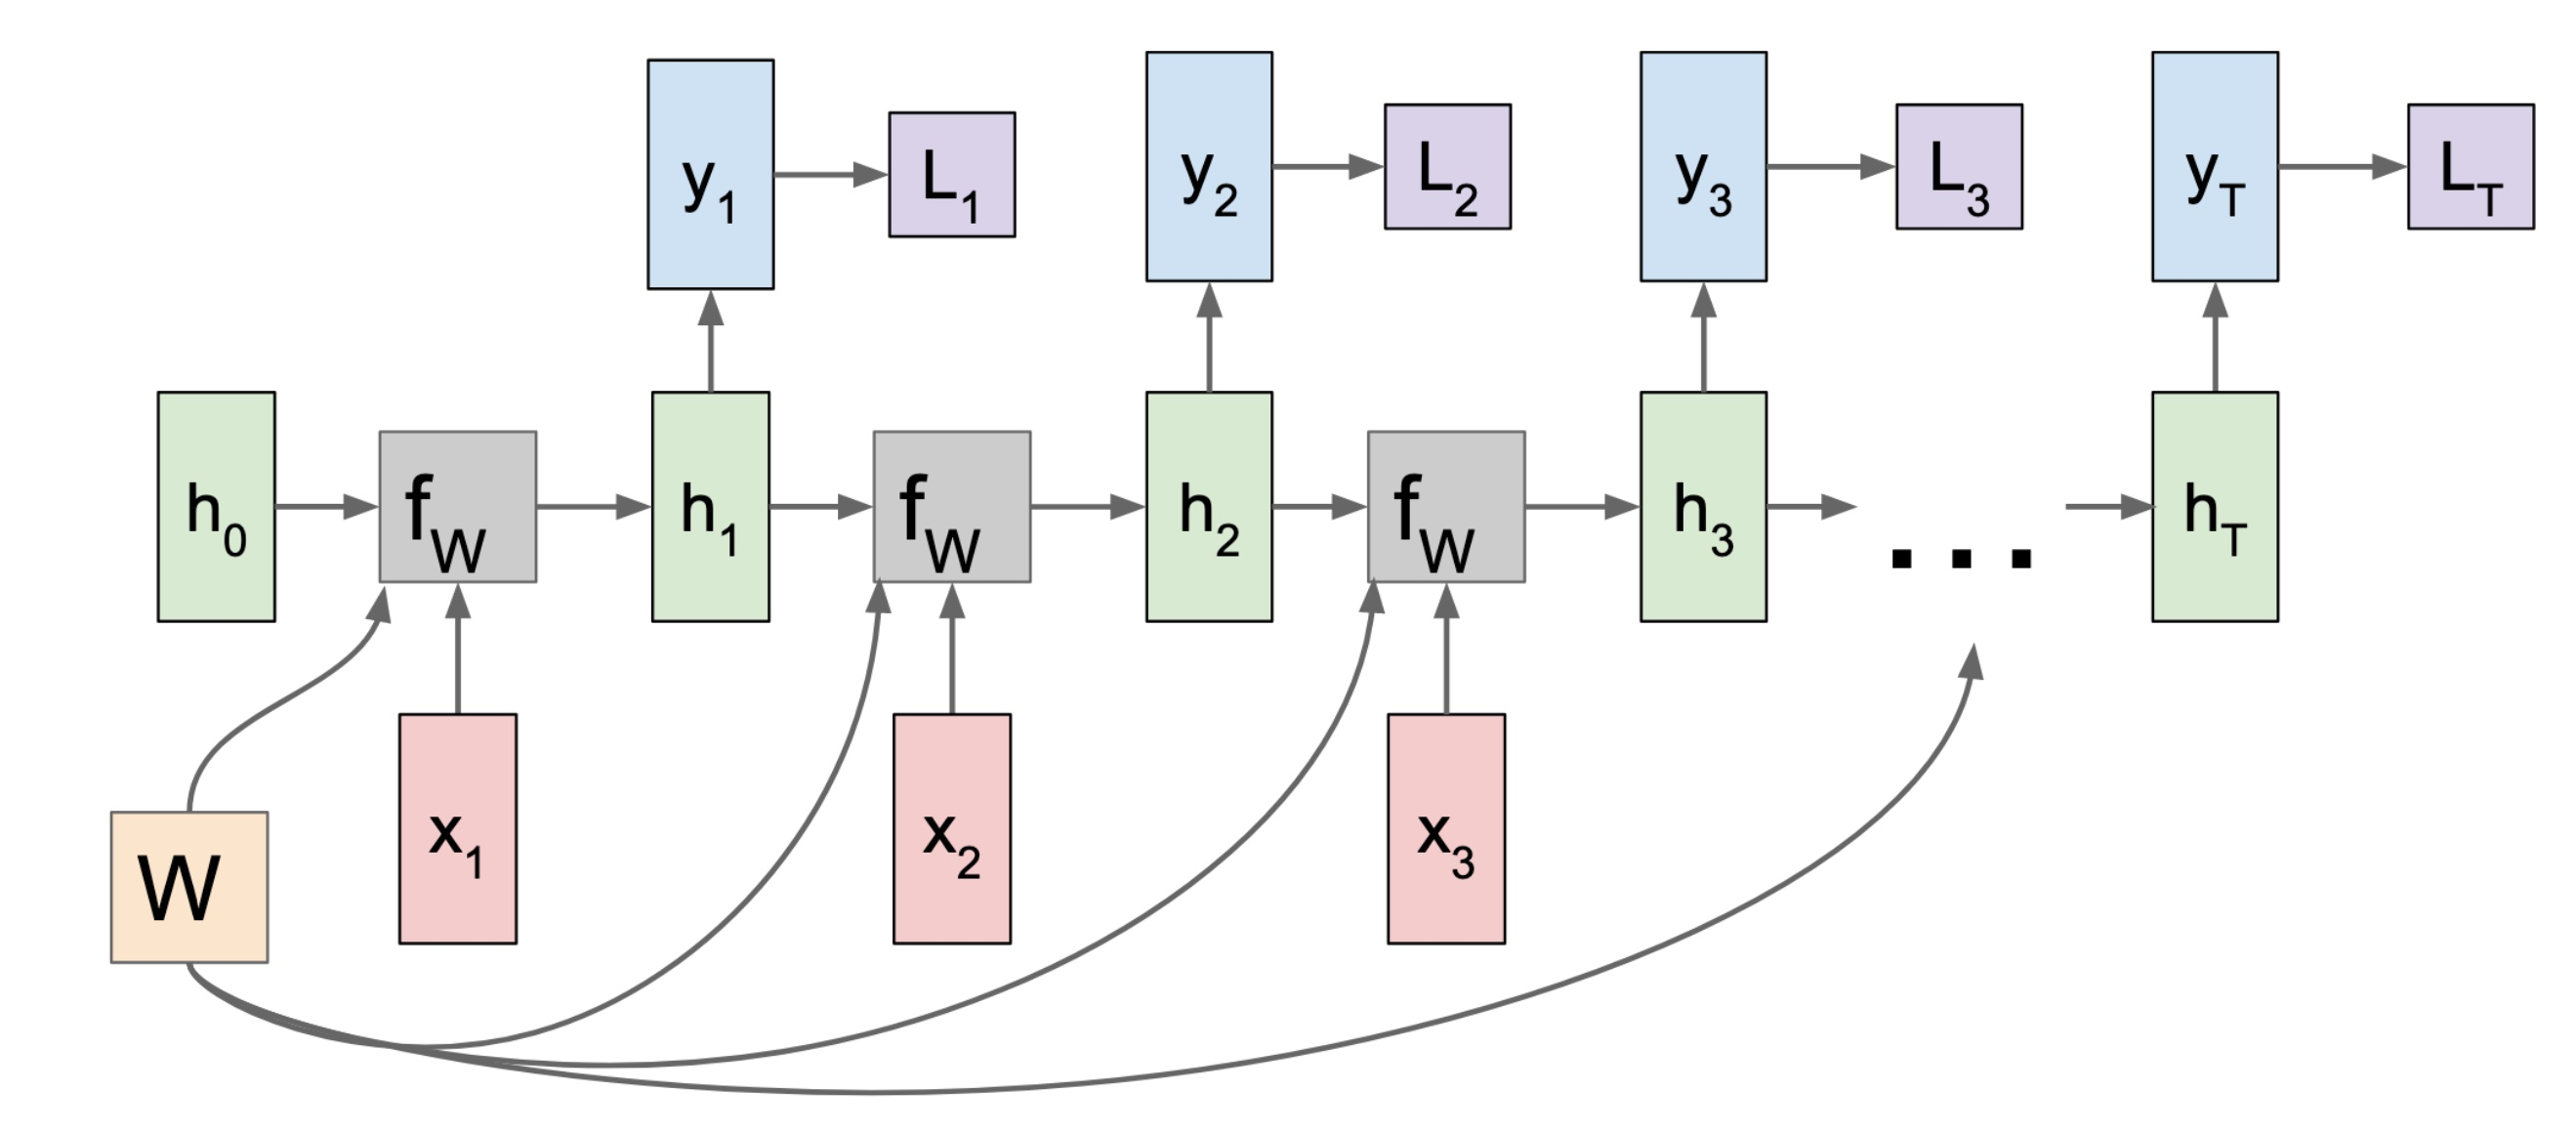
\includegraphics[width=\textwidth]{pics/rnngraph6}
\end{center}

\end{frame}

\begin{frame}

\frametitle{Recurrent Neural Network: Computational Graph}

\begin{center}
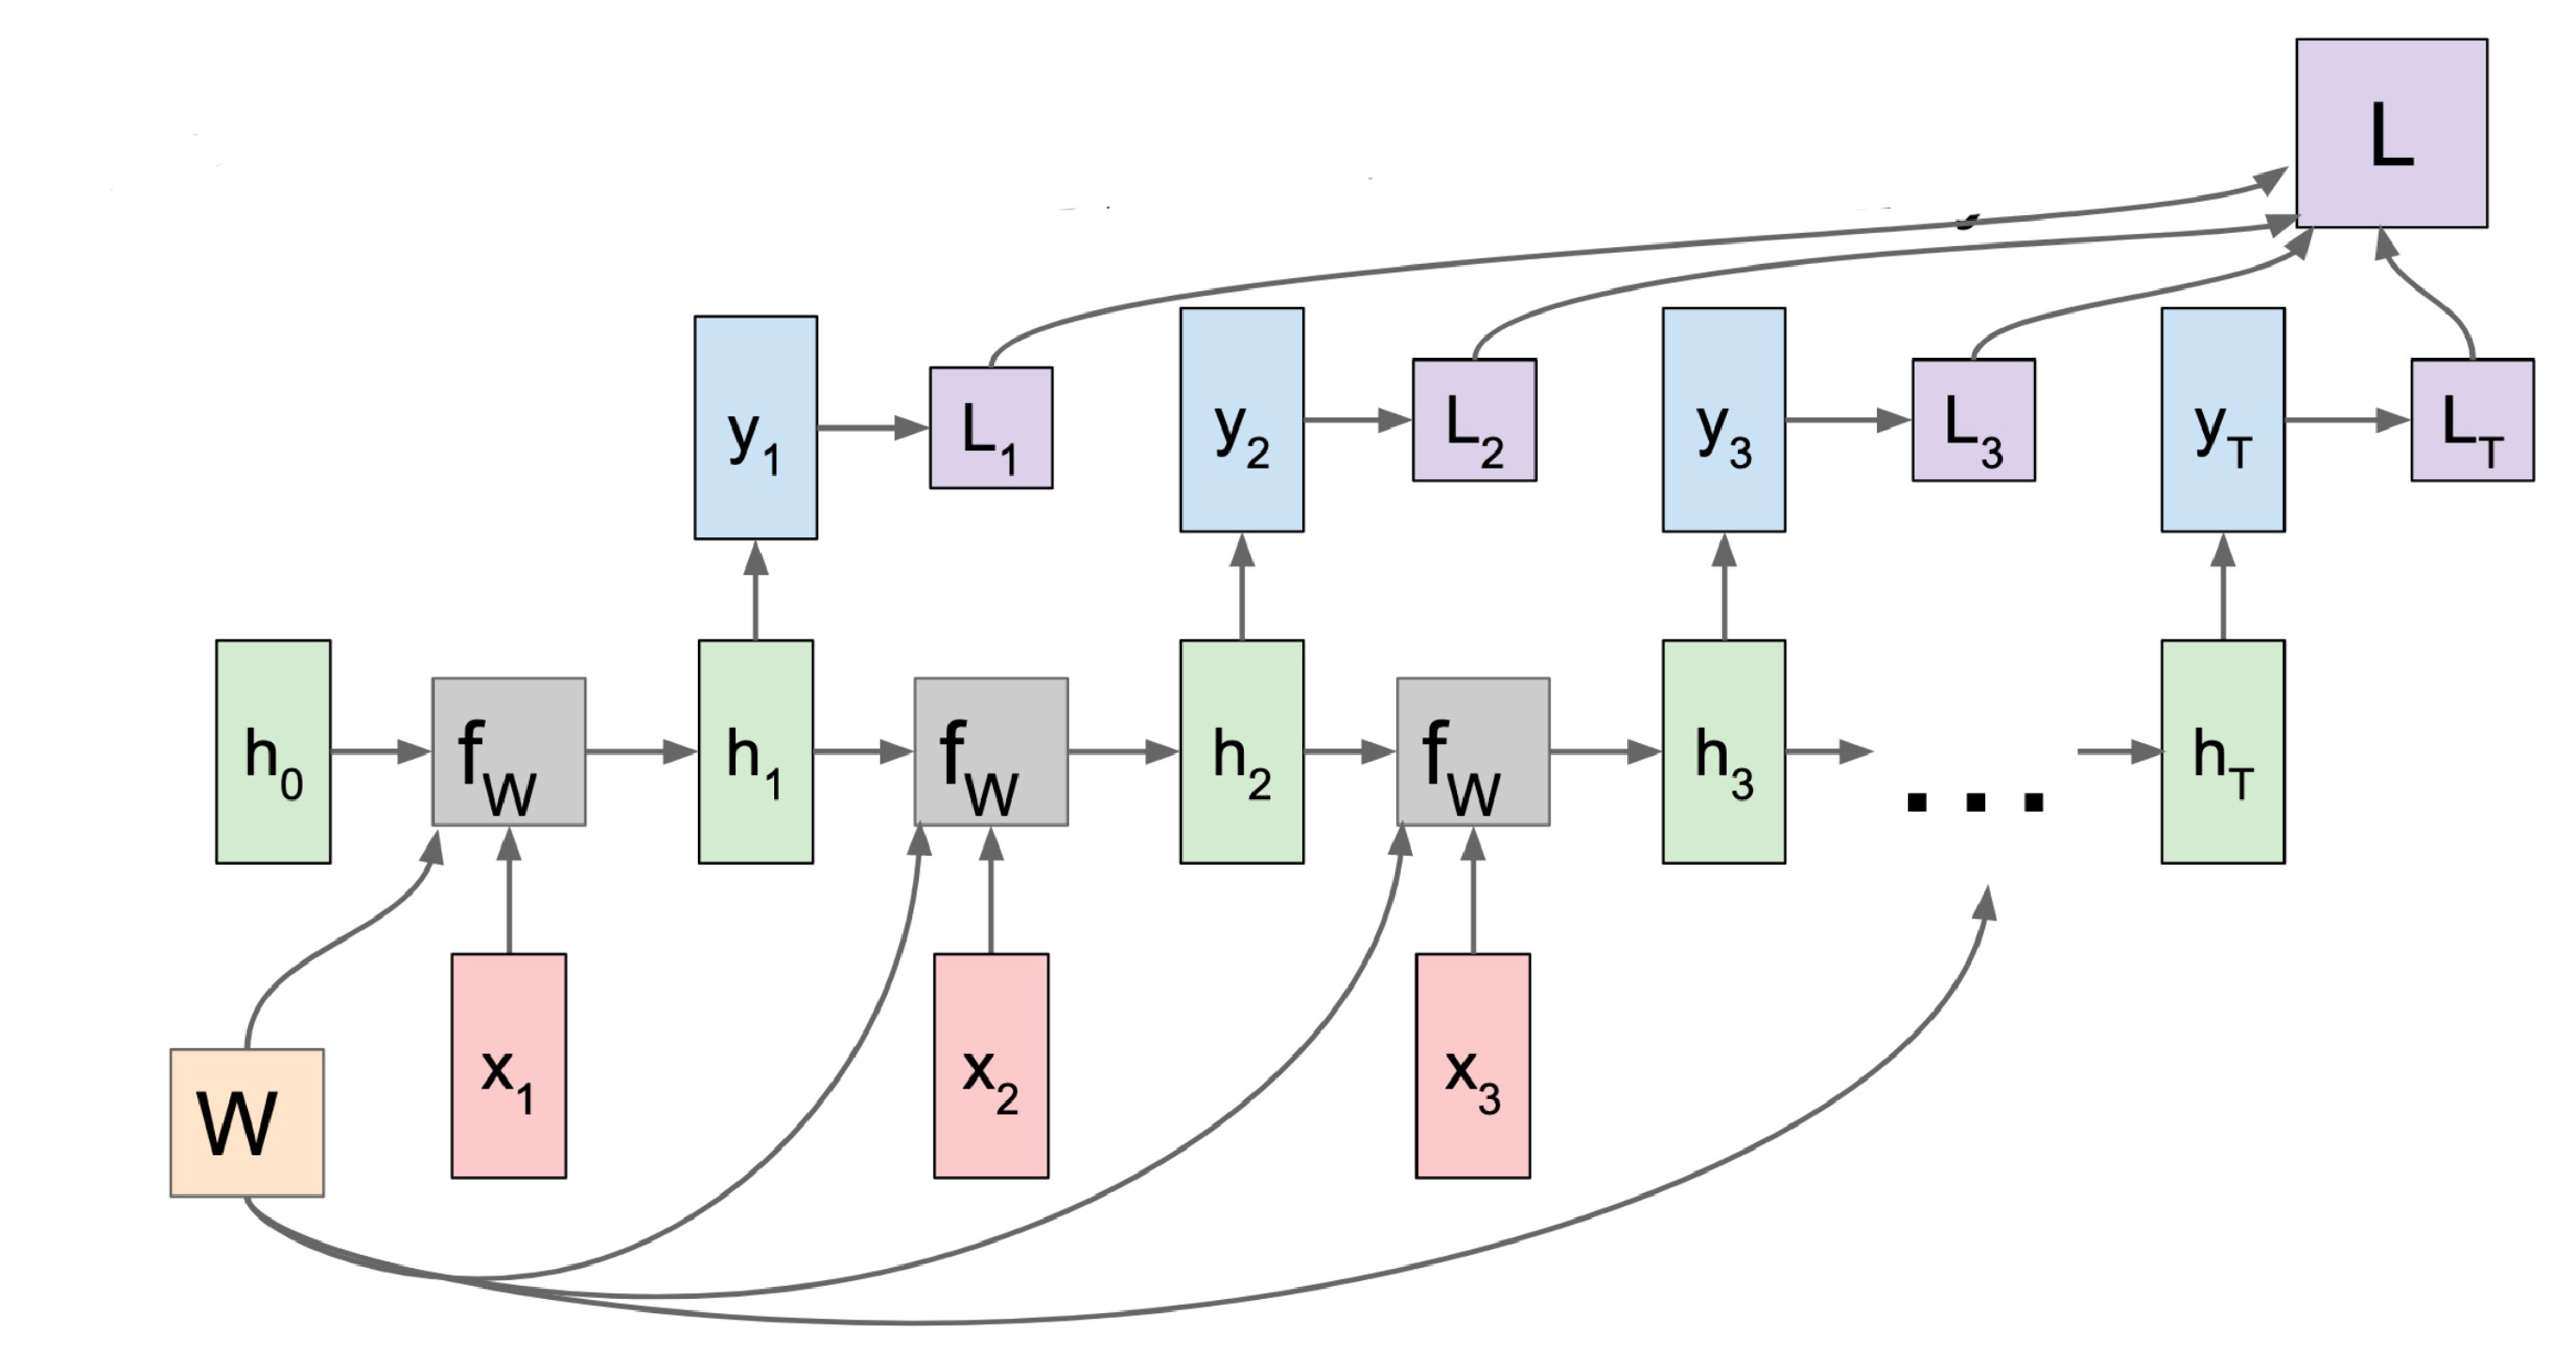
\includegraphics[width=.9\textwidth]{pics/rnngraph7}
\end{center}

\end{frame}

\begin{frame}

\frametitle{Recurrent Neural Network for Image Captioning}

\begin{center}
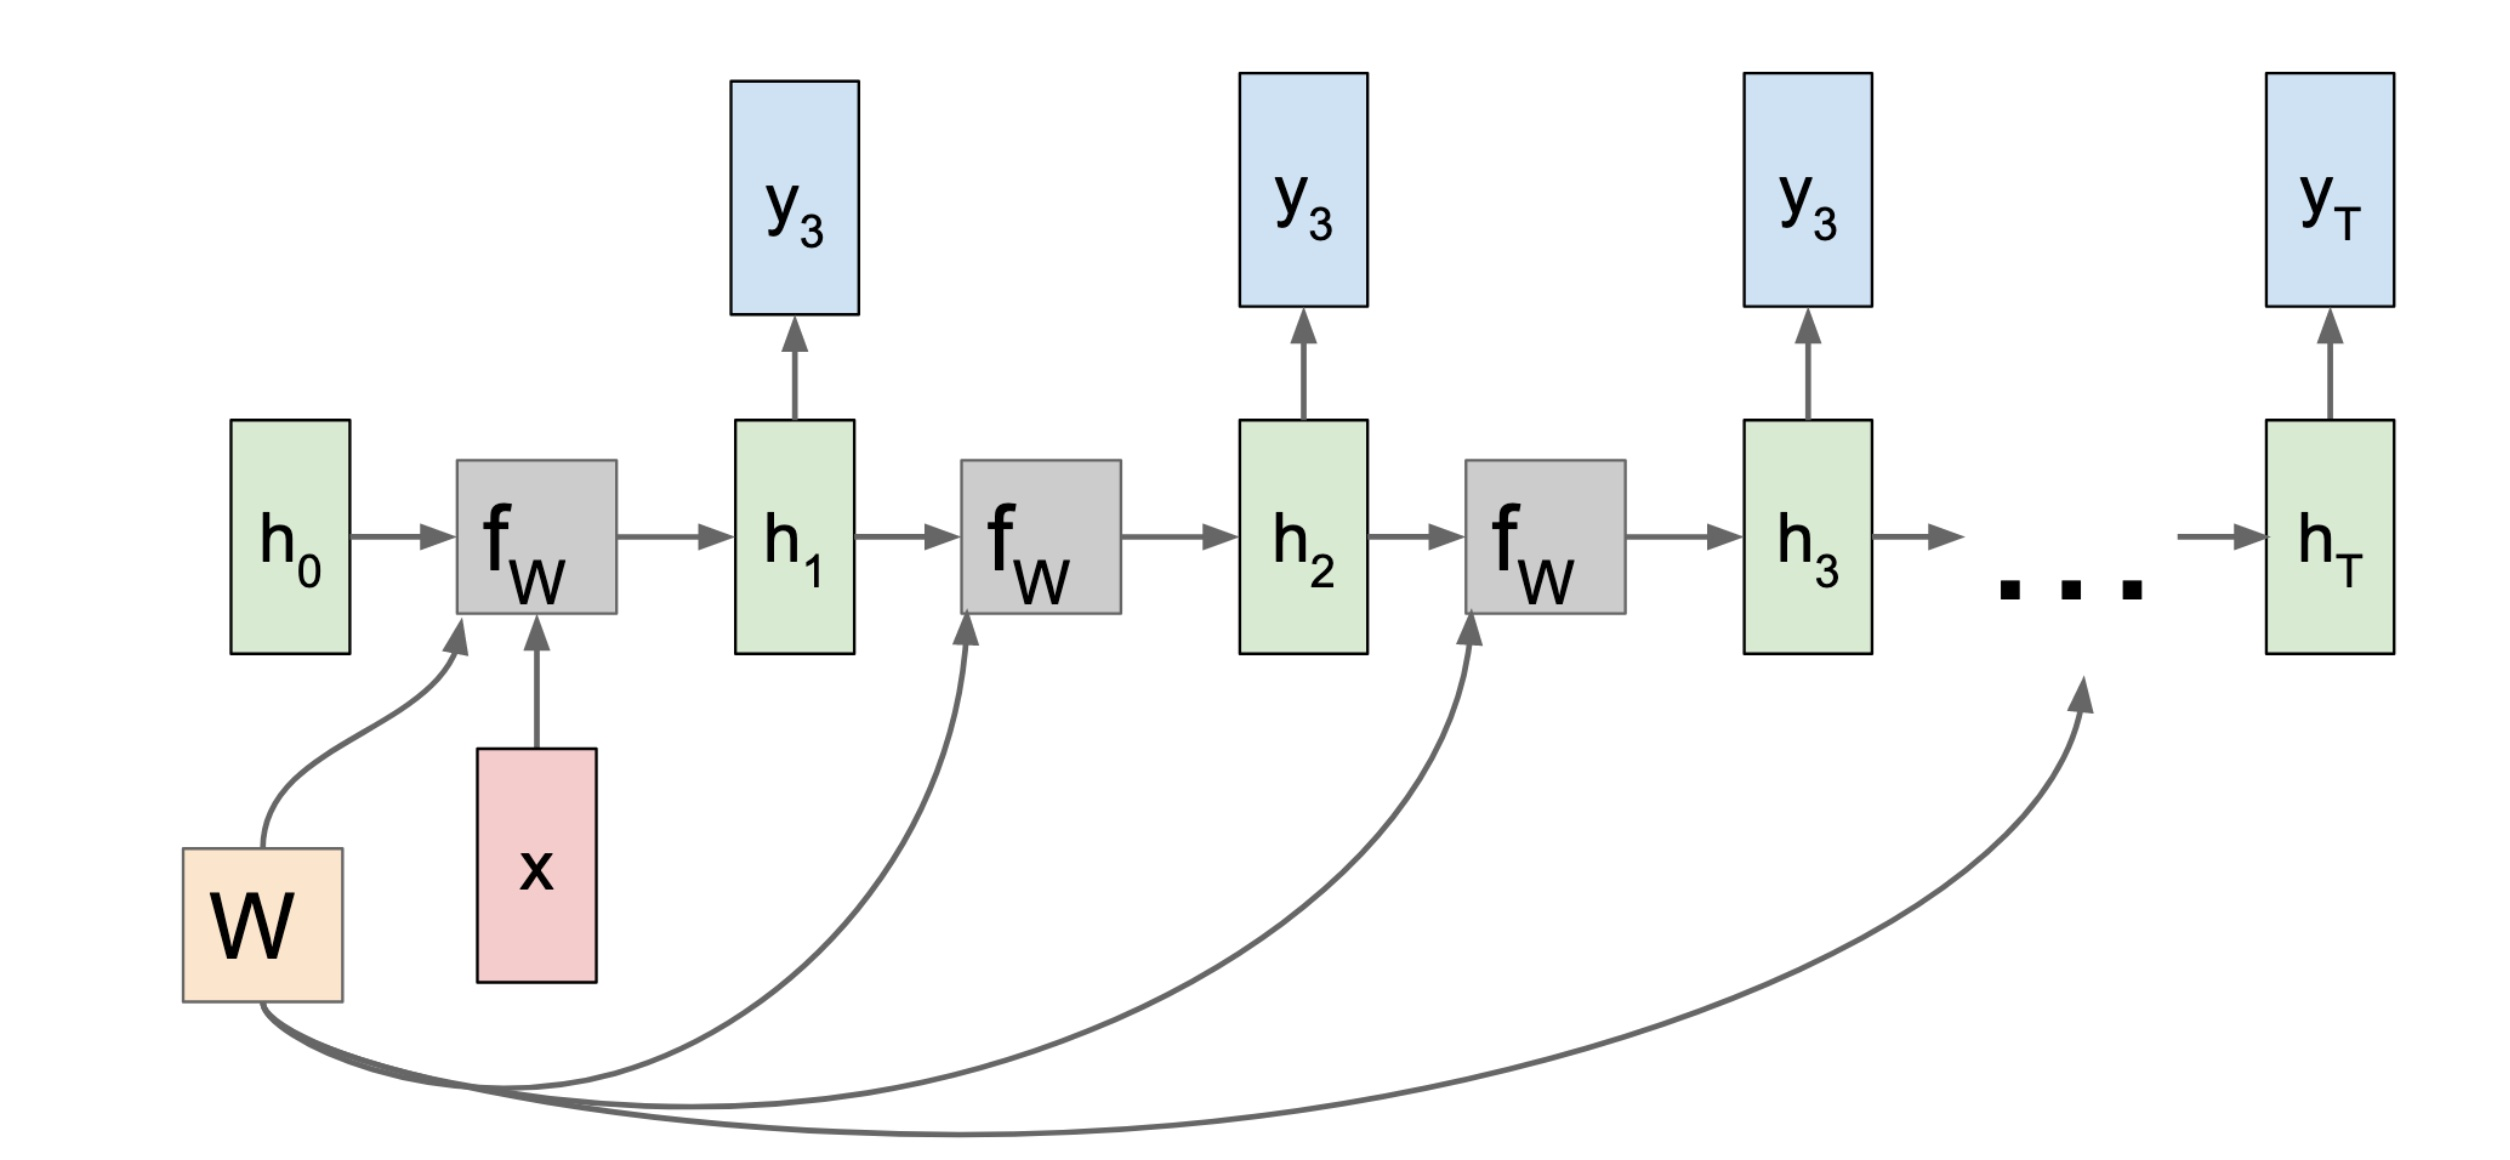
\includegraphics[width=.9\textwidth]{pics/rnngraph8}
\end{center}

\end{frame}


\begin{frame}

\frametitle{Example RNN: character-level generation}

\begin{center}
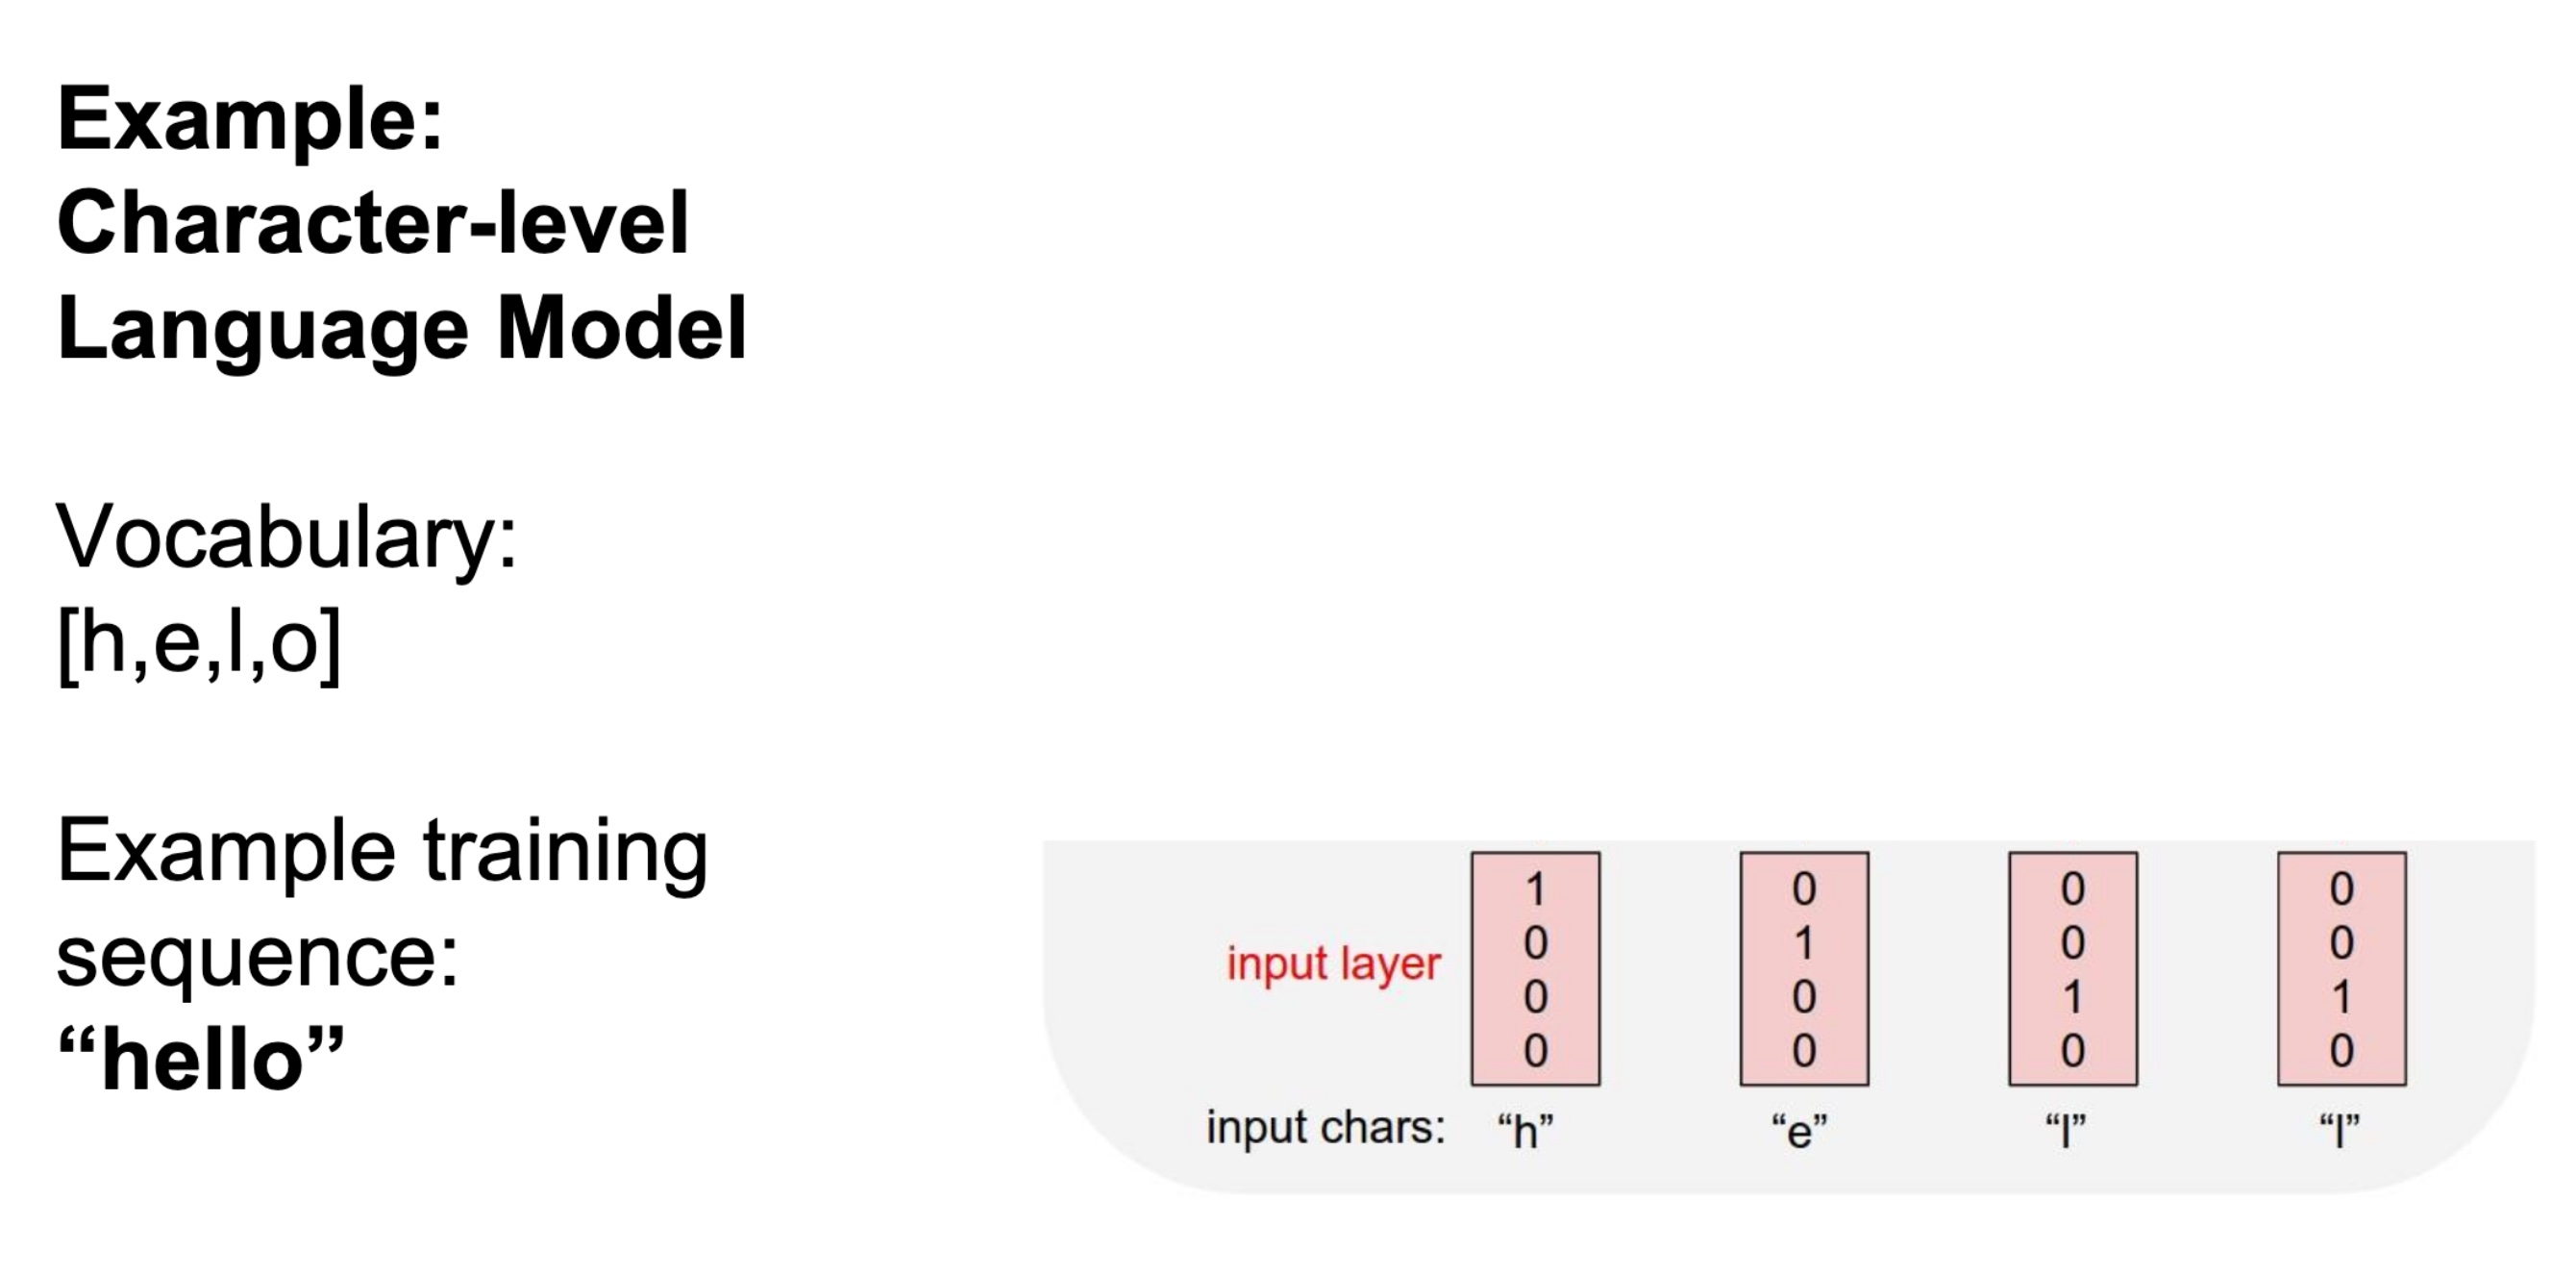
\includegraphics[width=\textwidth]{pics/example1}
\end{center}

\end{frame}

\begin{frame}

\frametitle{Example RNN: character-level generation}

\begin{center}
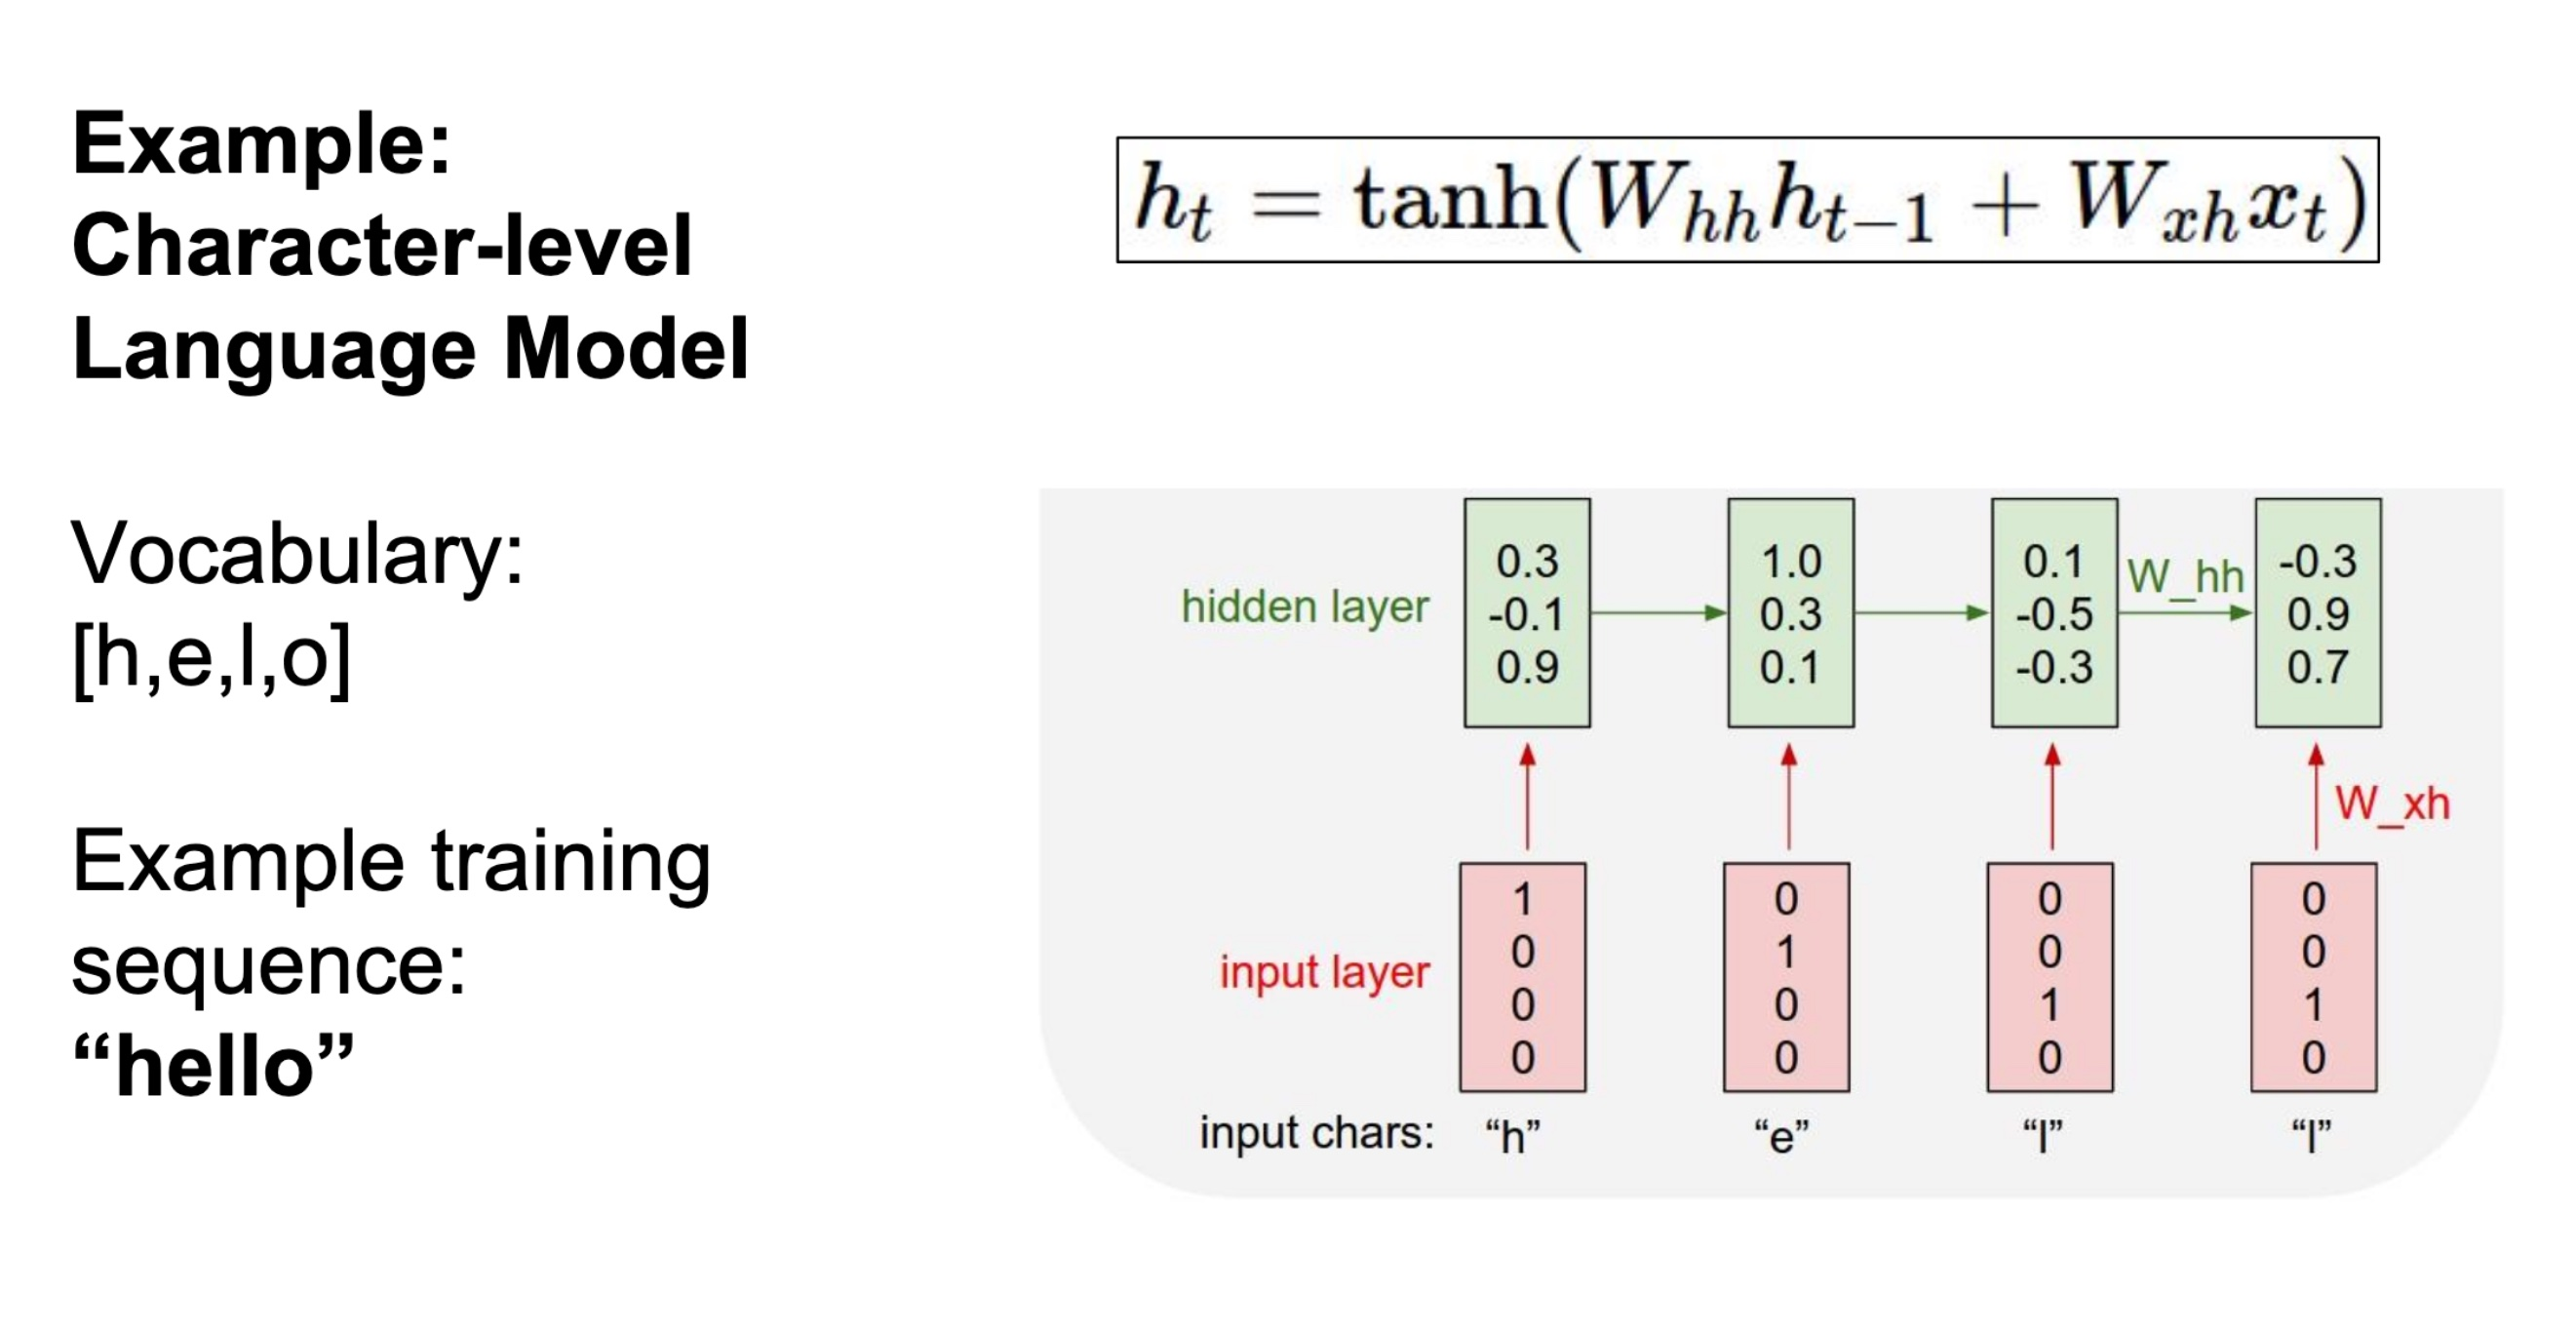
\includegraphics[width=\textwidth]{pics/example2}
\end{center}

\end{frame}


\begin{frame}

\frametitle{Example RNN: character-level generation}

\begin{center}
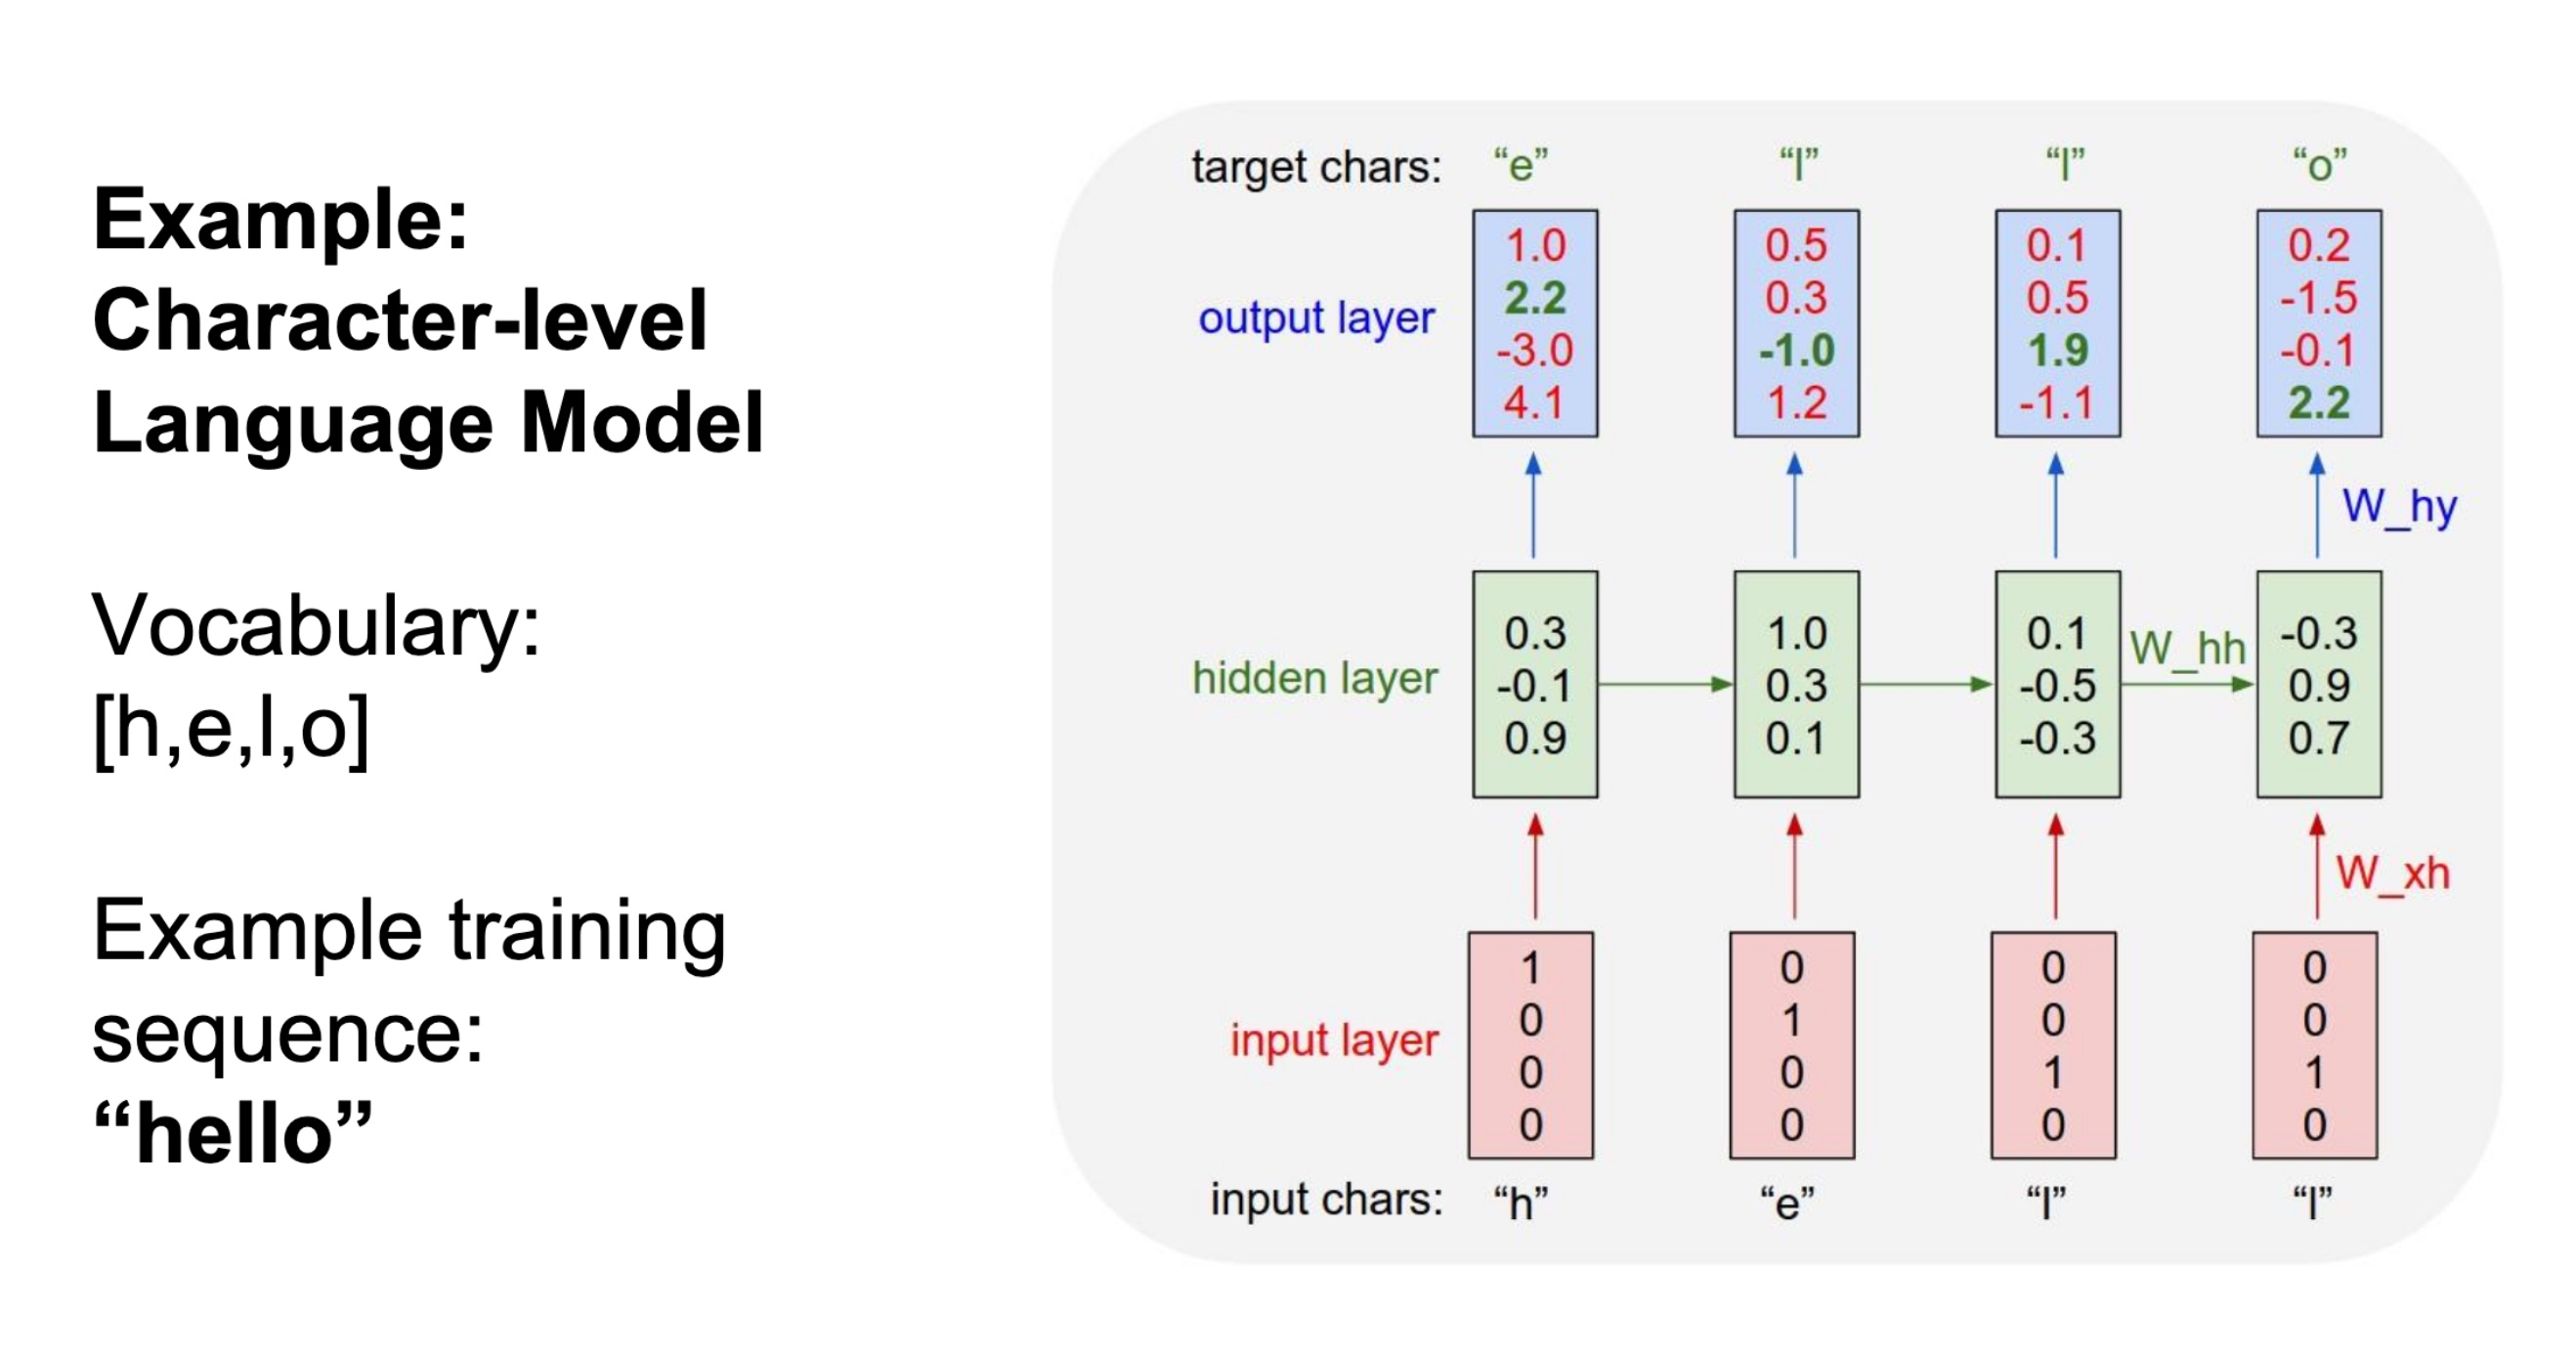
\includegraphics[width=\textwidth]{pics/example3}
\end{center}

\end{frame}

\begin{frame}

\frametitle{Example RNN: character-level generation}

\begin{center}
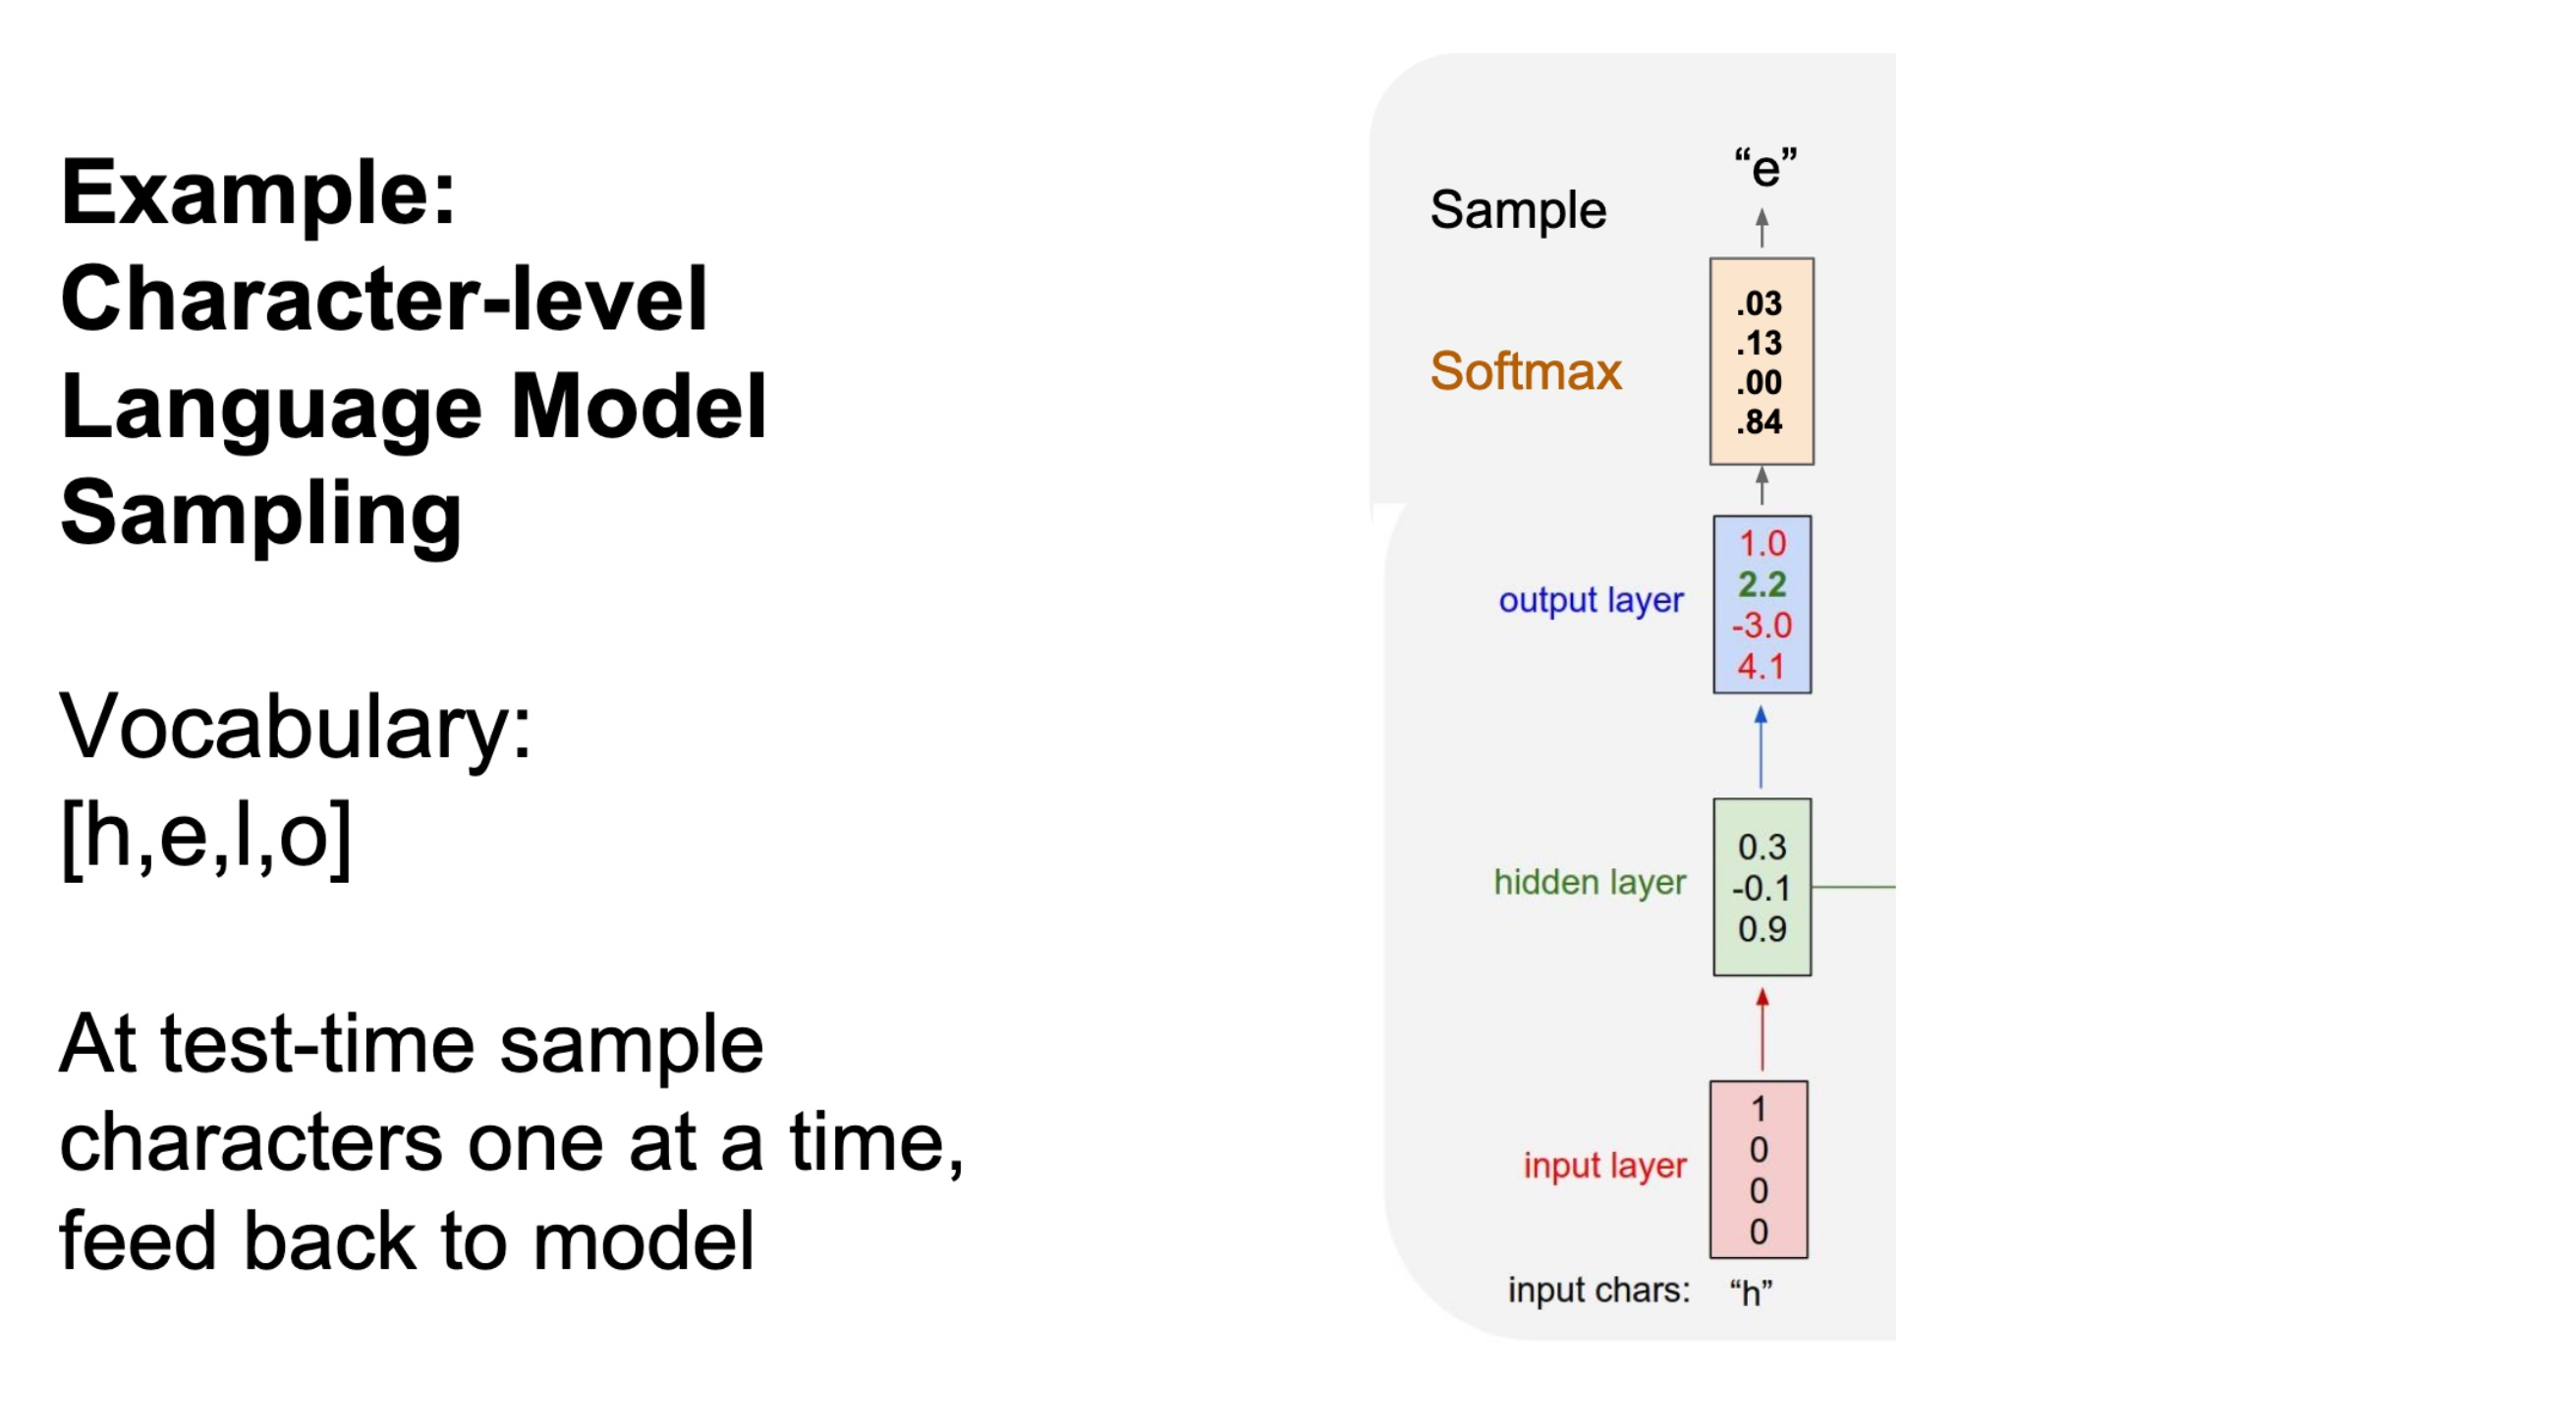
\includegraphics[width=\textwidth]{pics/example4}
\end{center}

\end{frame}


\begin{frame}

\frametitle{Example RNN: character-level generation}

\begin{center}
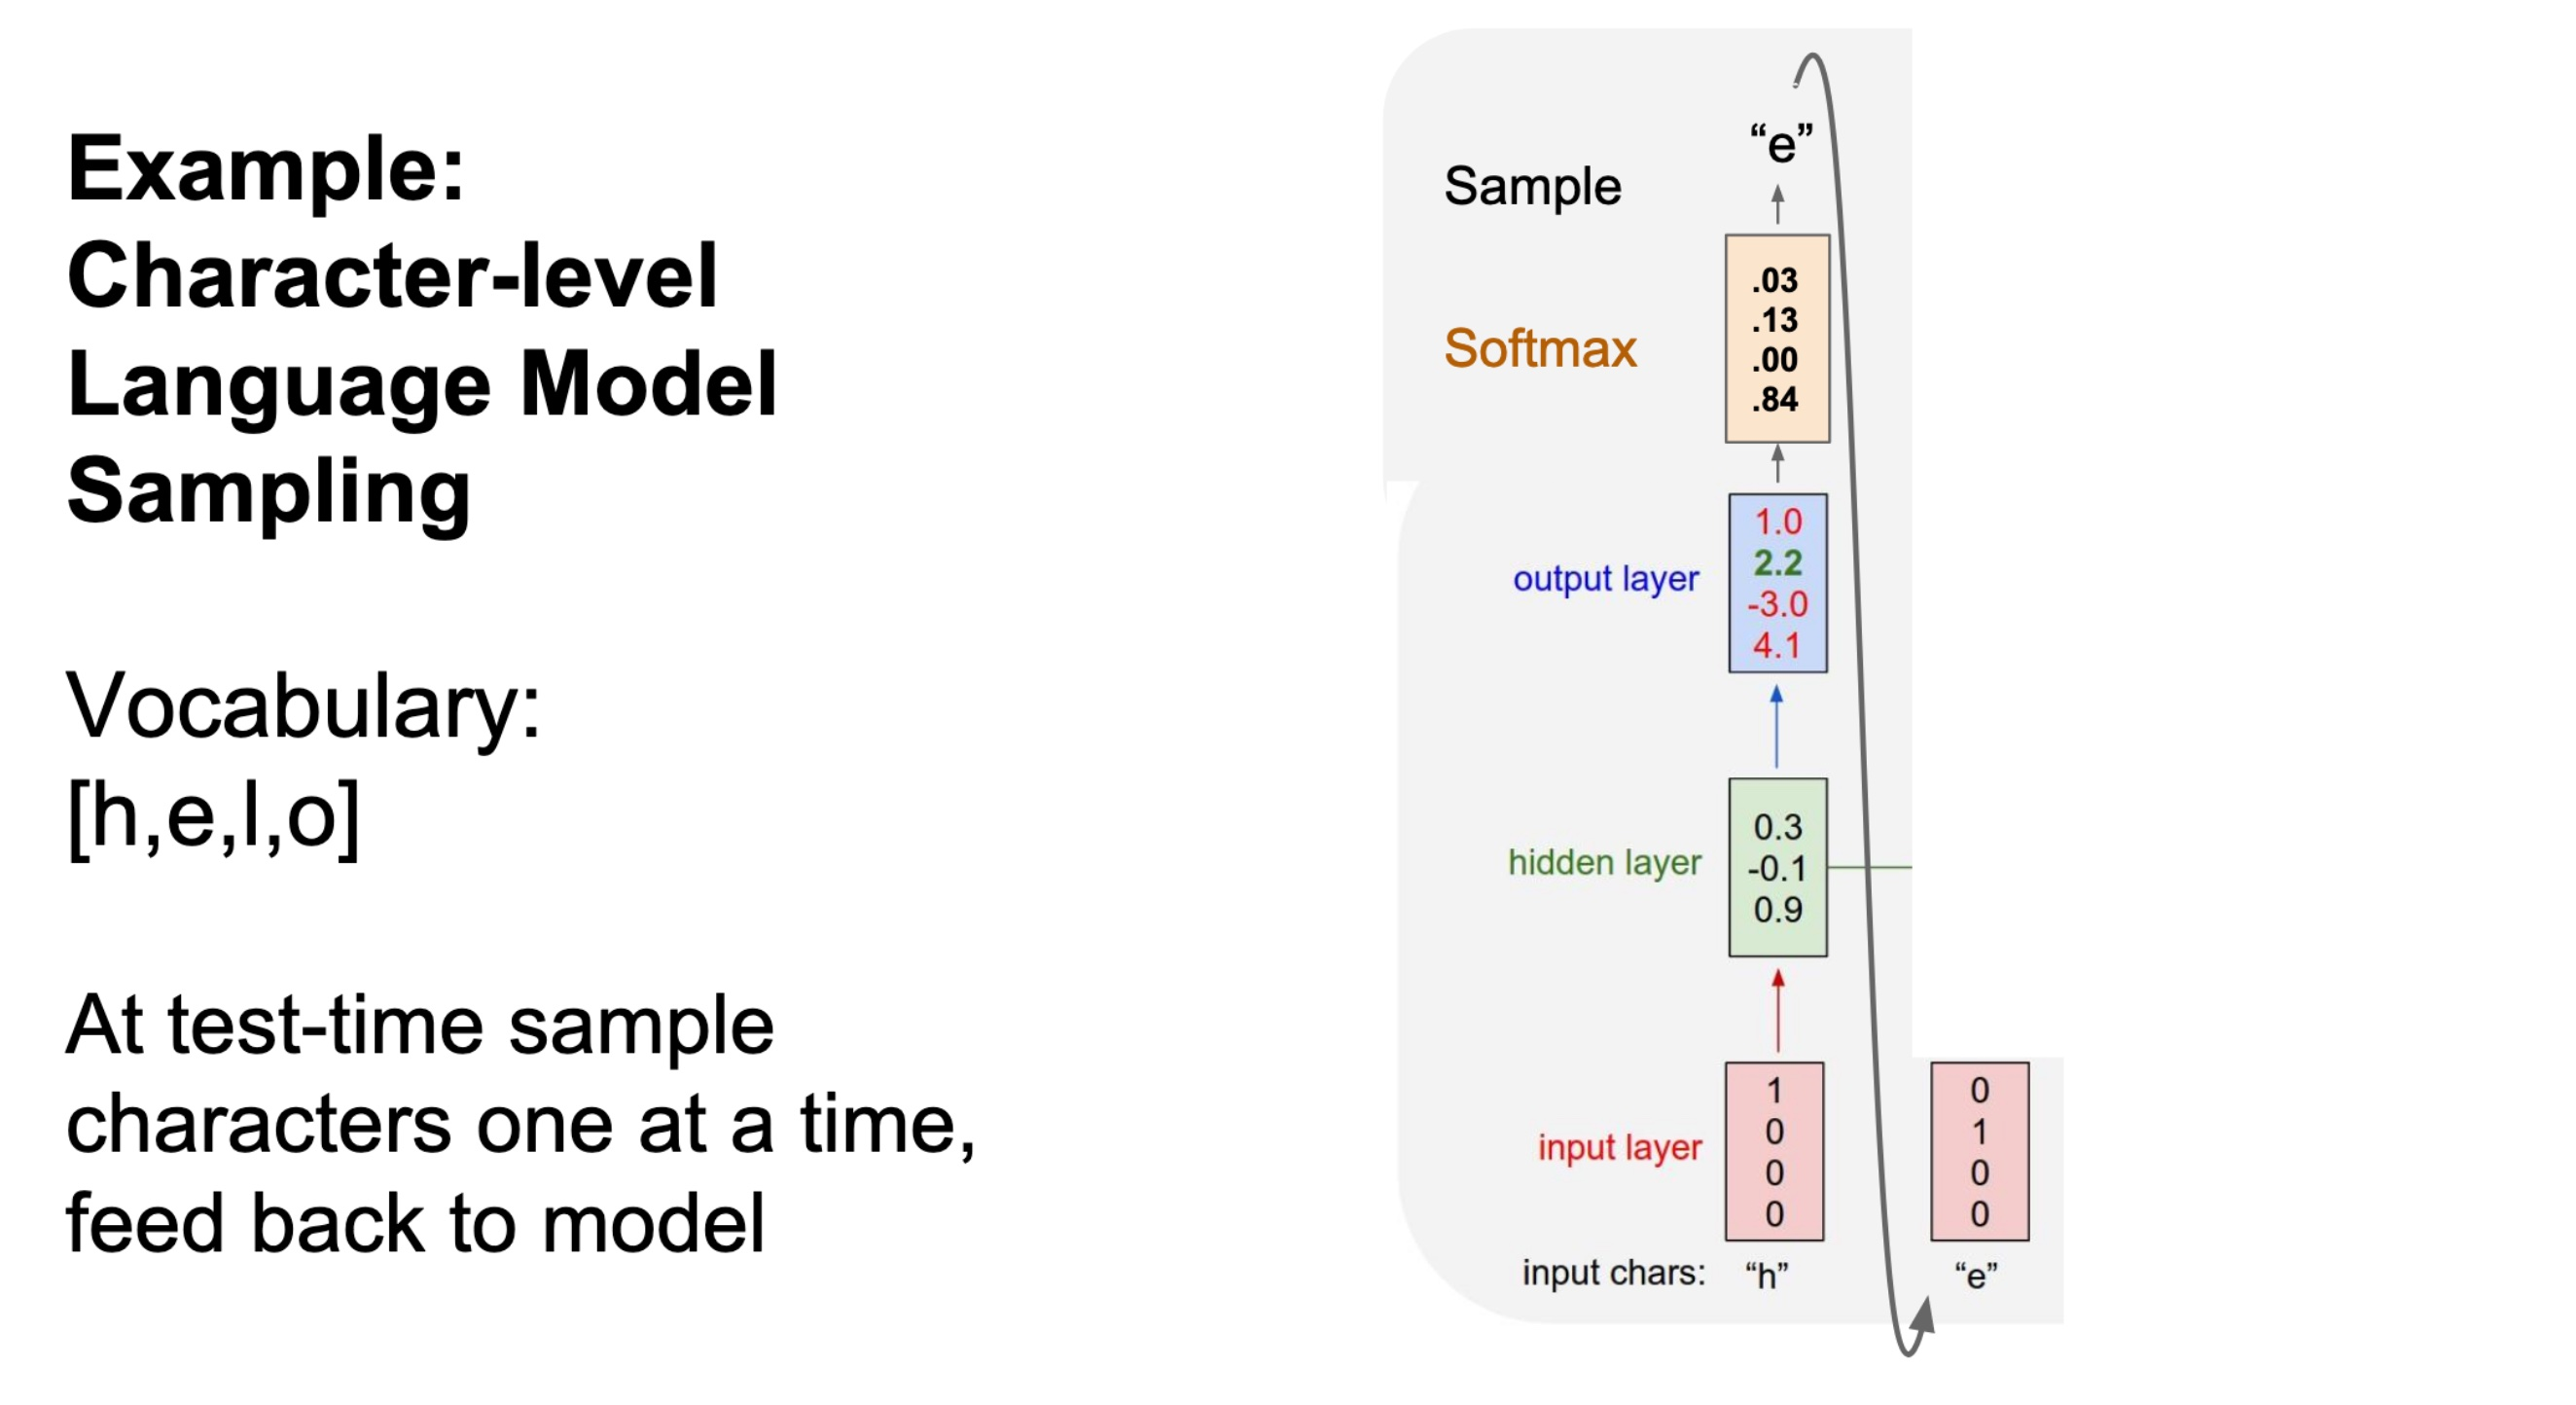
\includegraphics[width=\textwidth]{pics/example5}
\end{center}

\end{frame}

\begin{frame}

\frametitle{Example RNN: character-level generation}

\begin{center}
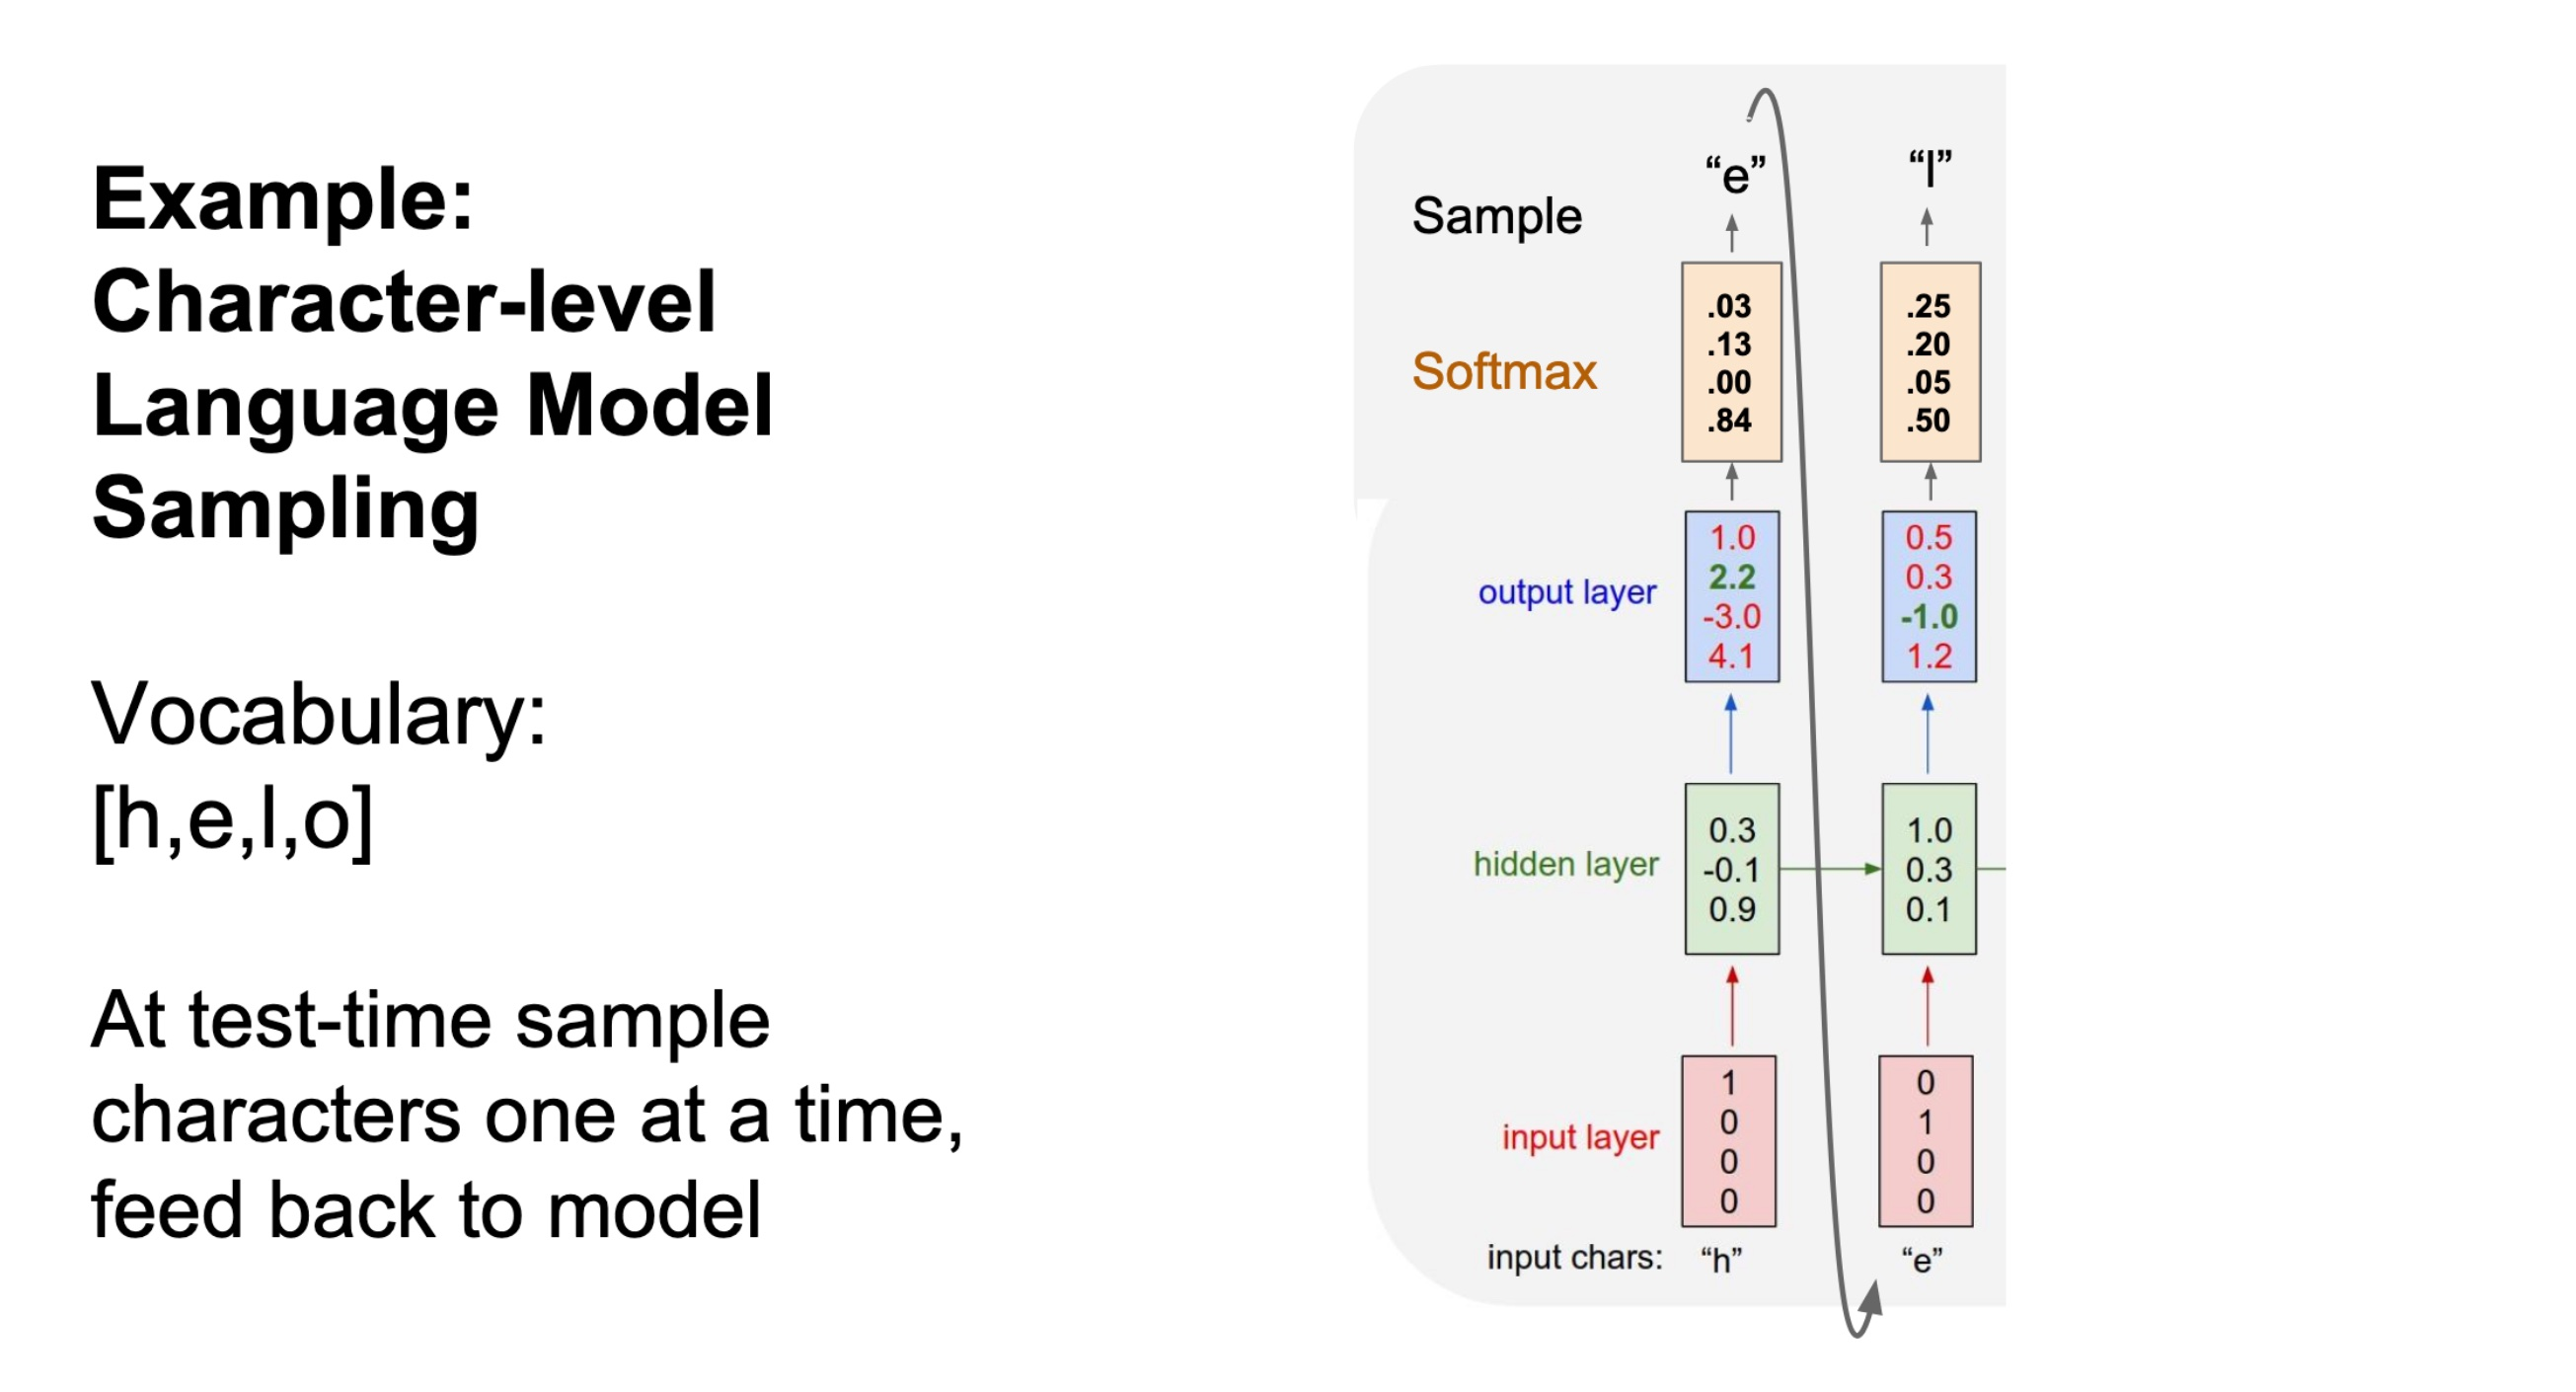
\includegraphics[width=\textwidth]{pics/example6}
\end{center}

\end{frame}

\begin{frame}

\frametitle{Example RNN: character-level generation}

\begin{center}
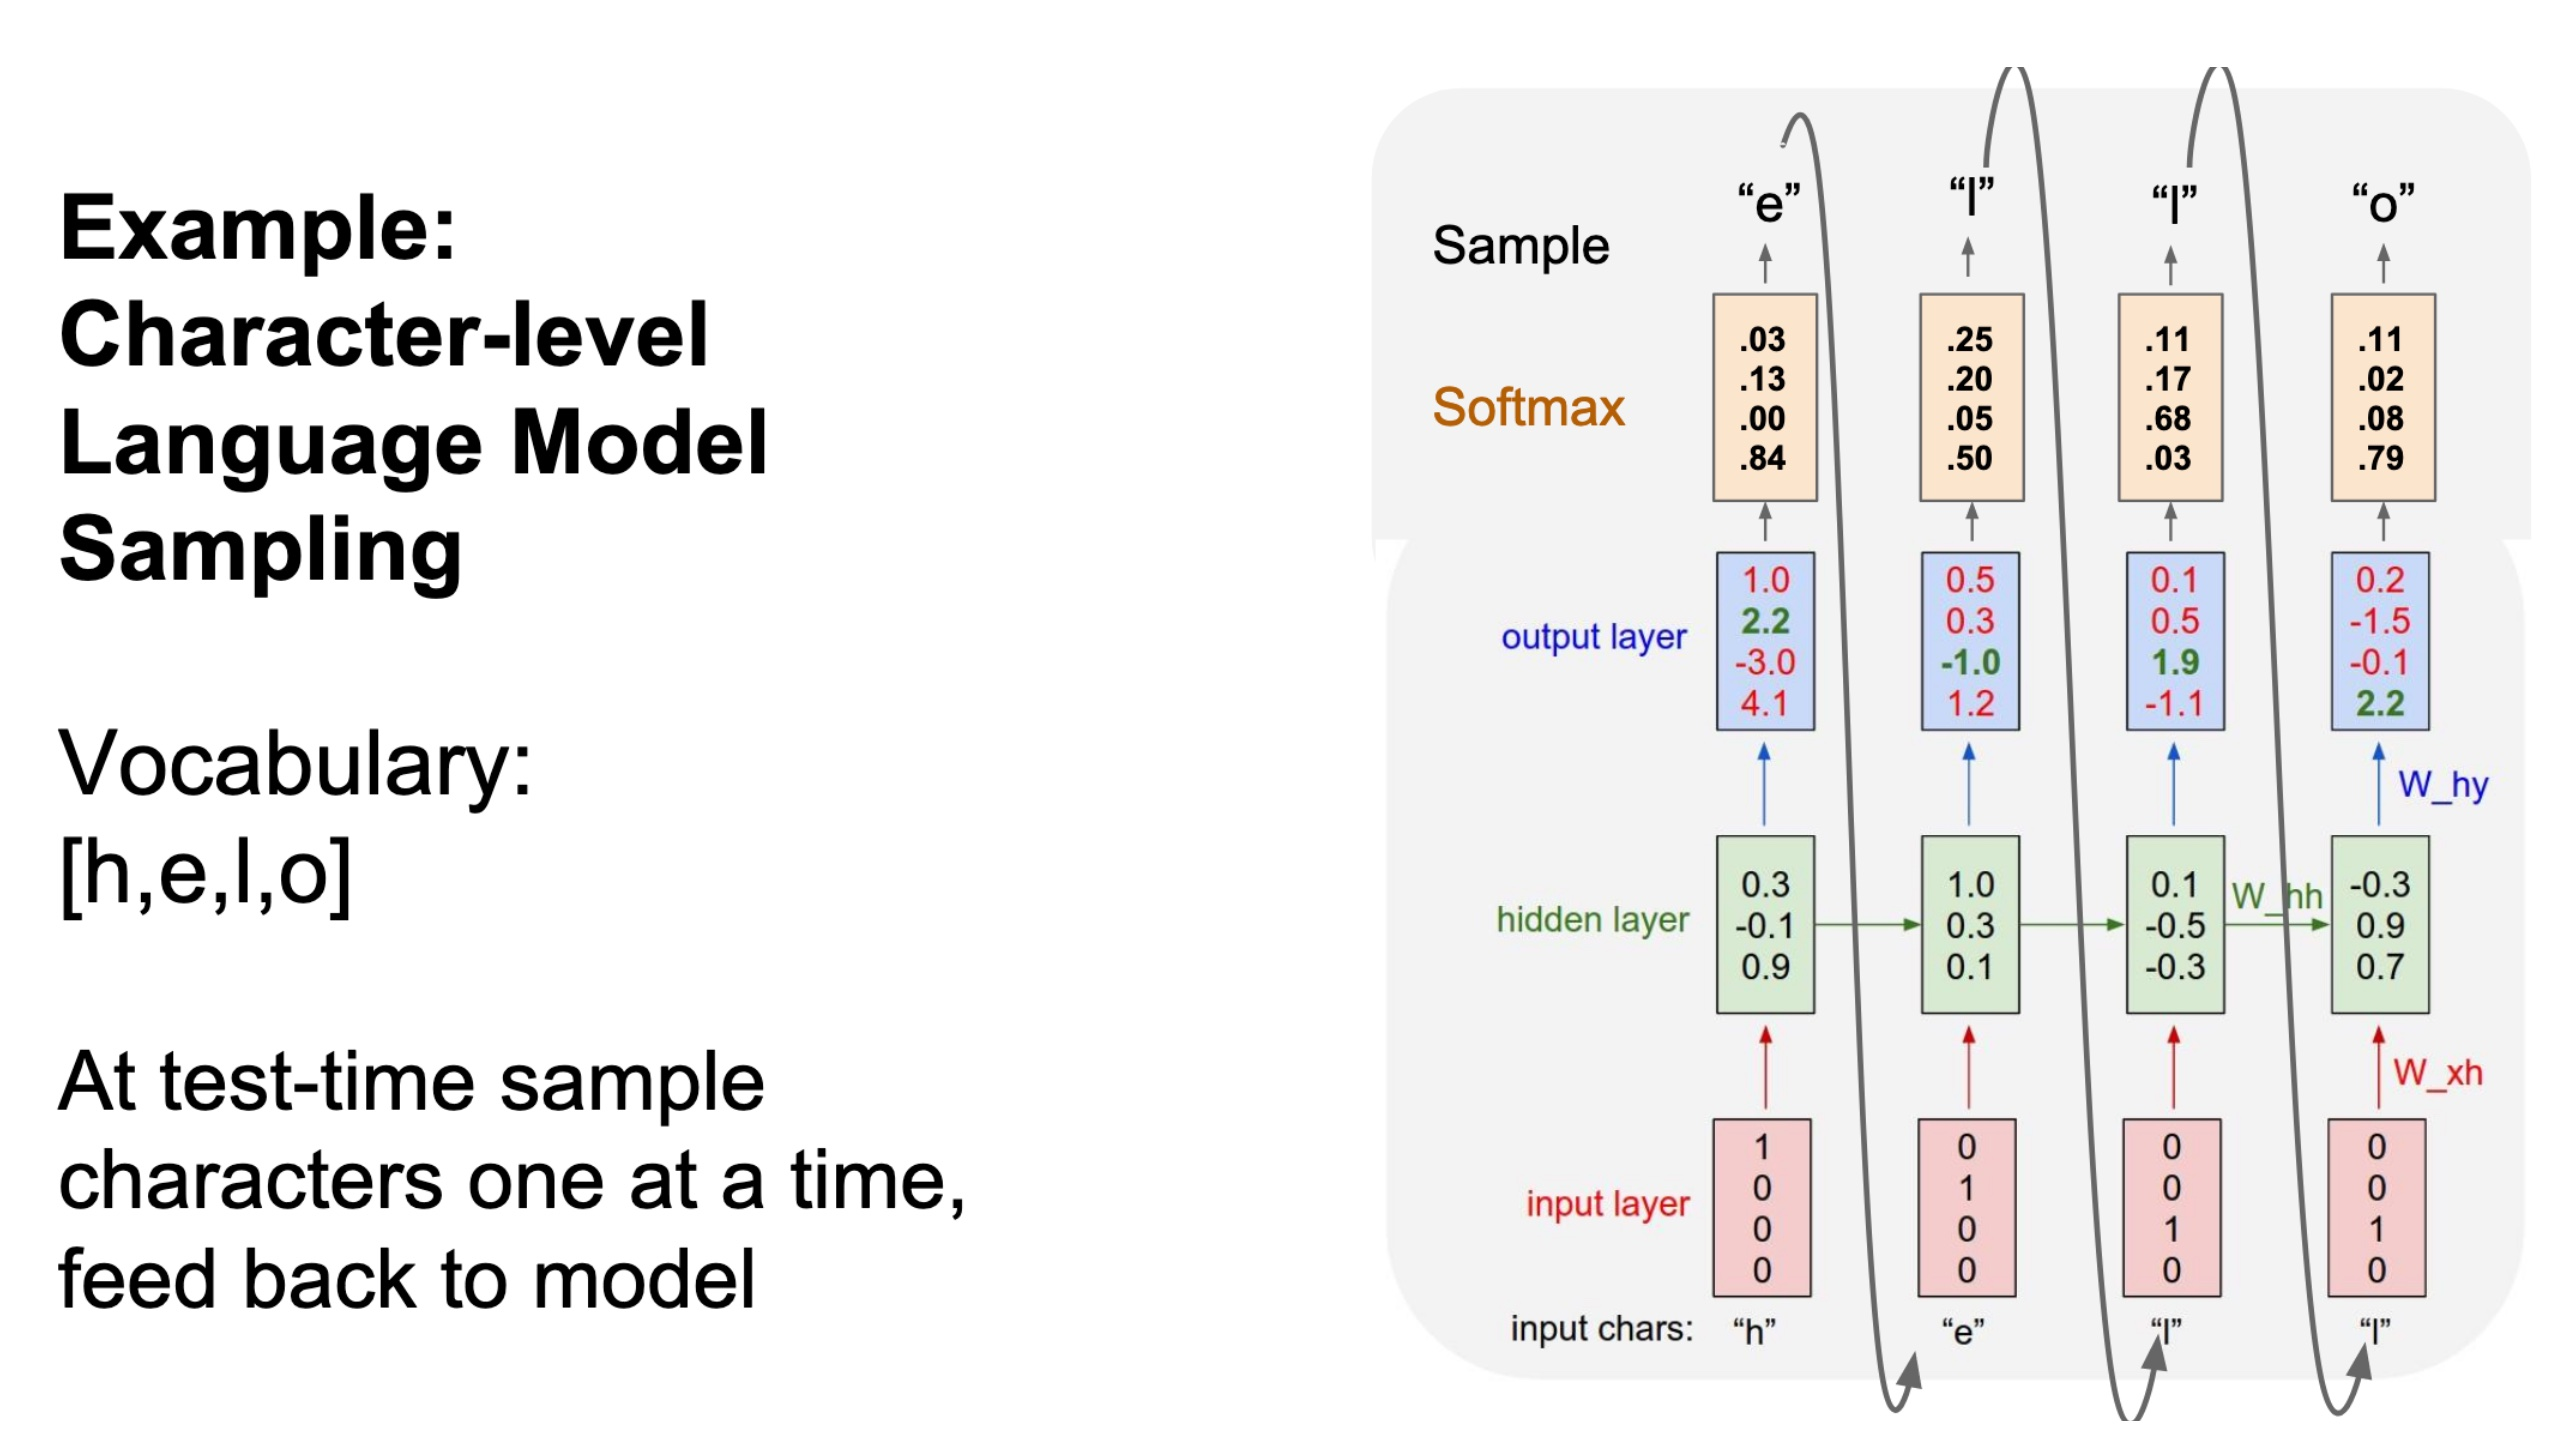
\includegraphics[width=.9\textwidth]{pics/example7}
\end{center}

\end{frame}


\begin{frame}

\frametitle{Image Captioning}


Classic literature on neural image captioning: \\\citet{mao2014explain,karpathy2015deep,vinyals2015tell,donahue2016longterm,chen2014learning}

\begin{center}
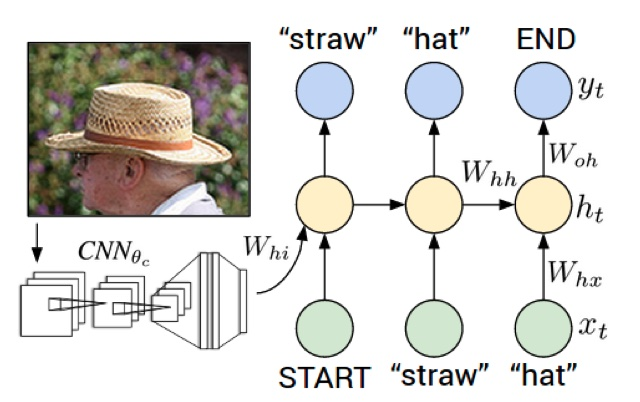
\includegraphics[width=.7\textwidth]{pics/hat}
\end{center}

\end{frame}


\begin{frame}
\frametitle{Image Captioning: how do we do it?}
\begin{center}
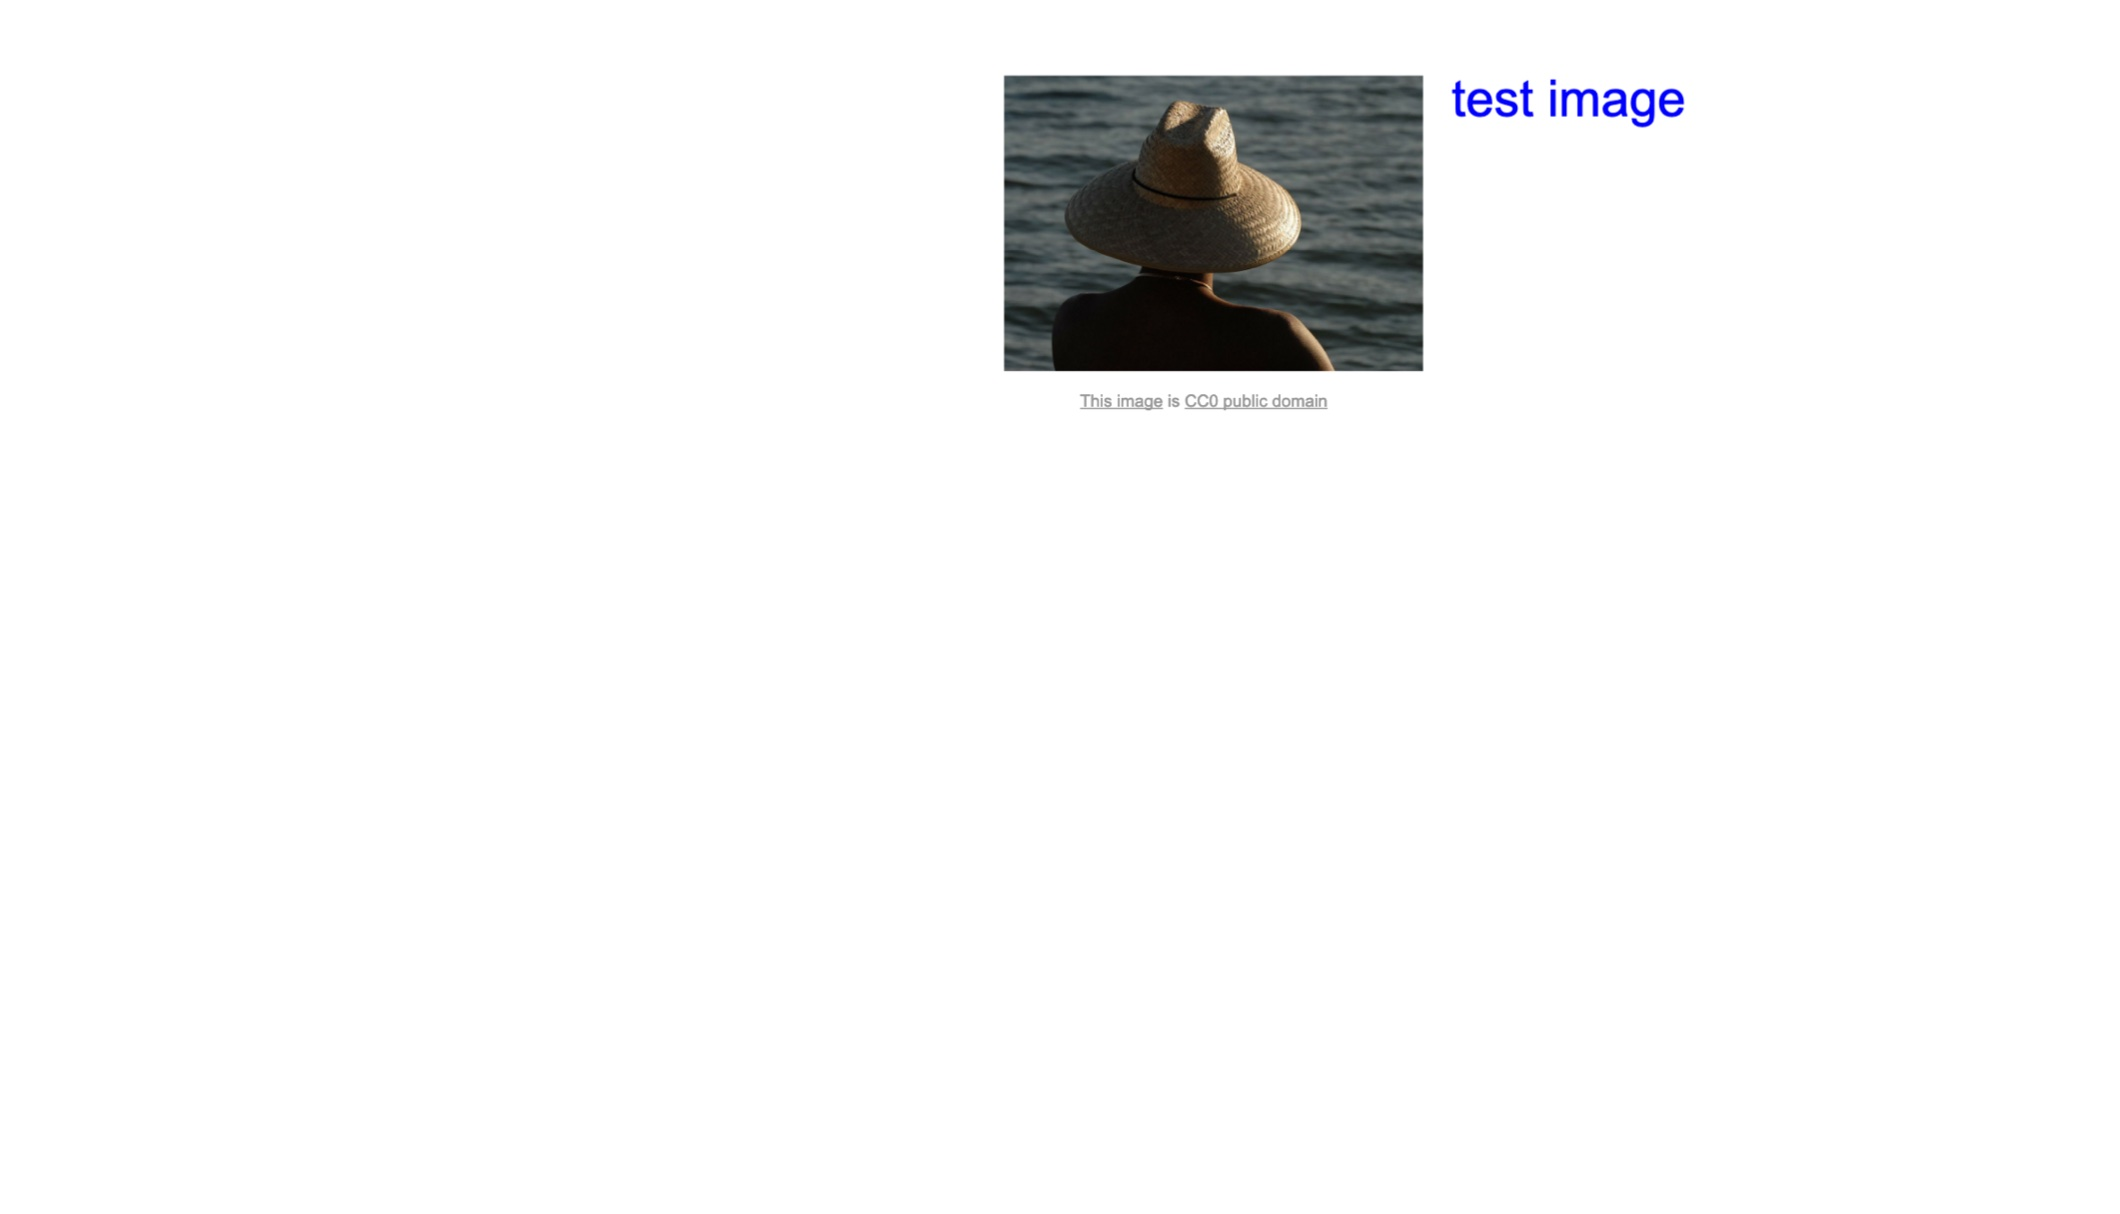
\includegraphics[width=.9\textwidth]{pics/cap1}
\end{center}
\end{frame}


\begin{frame}
\frametitle{Image Captioning: how do we do it?}
\begin{center}
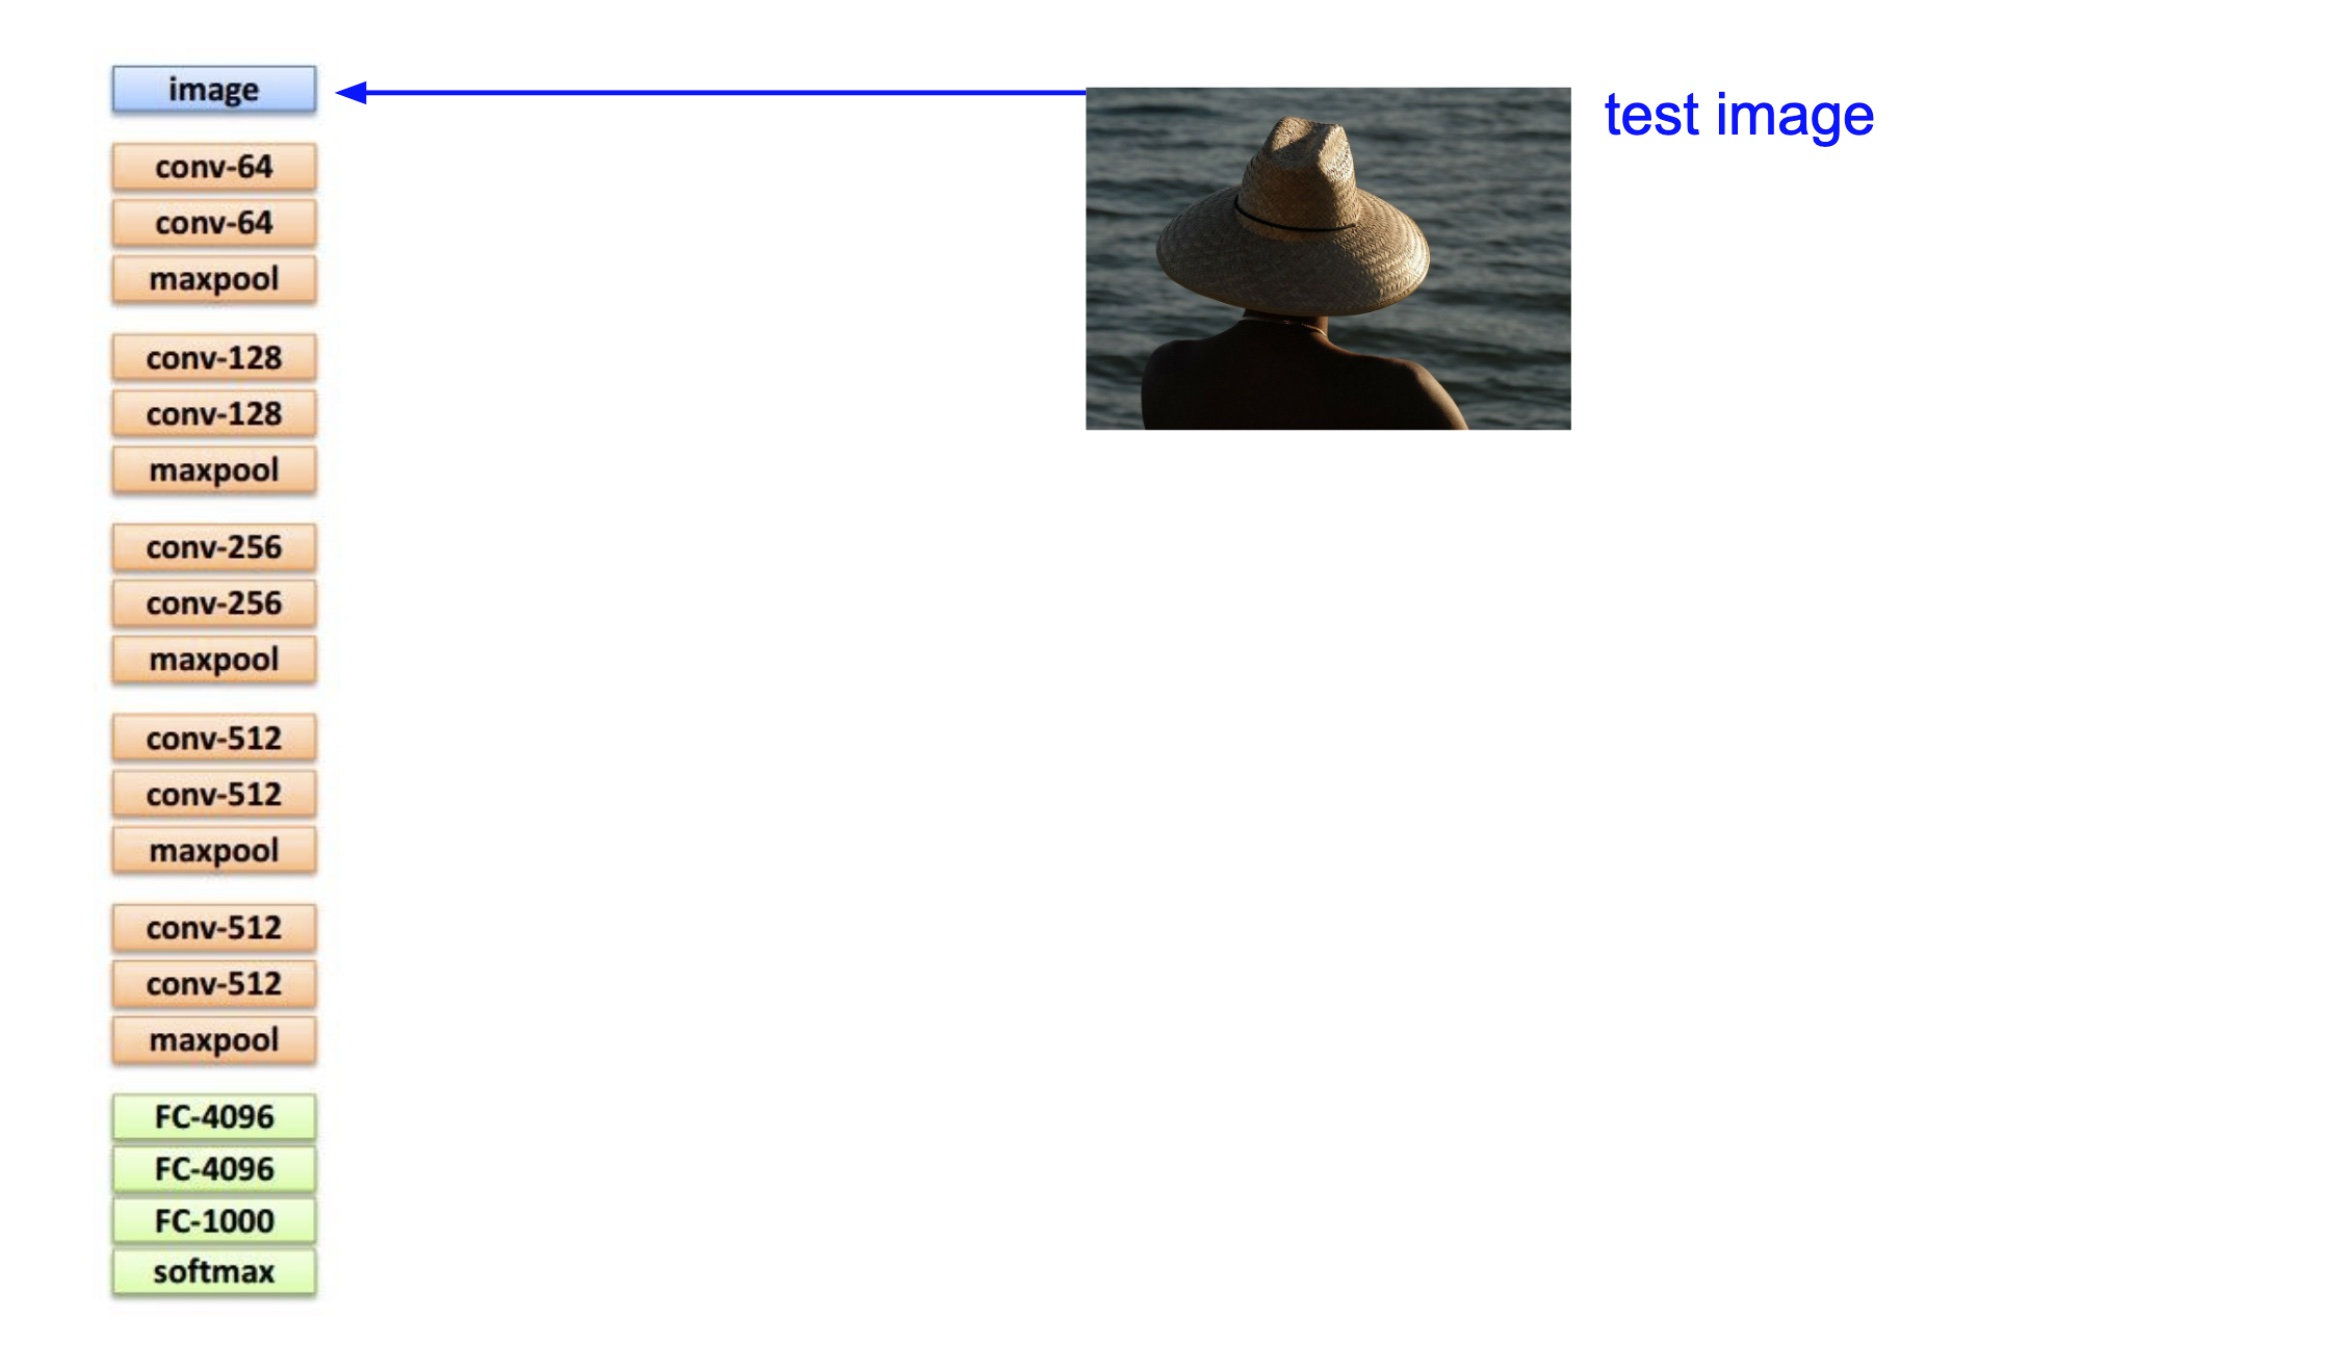
\includegraphics[width=.9\textwidth]{pics/cap2}
\end{center}
\end{frame}


\begin{frame}
\frametitle{Image Captioning: how do we do it?}
\begin{center}
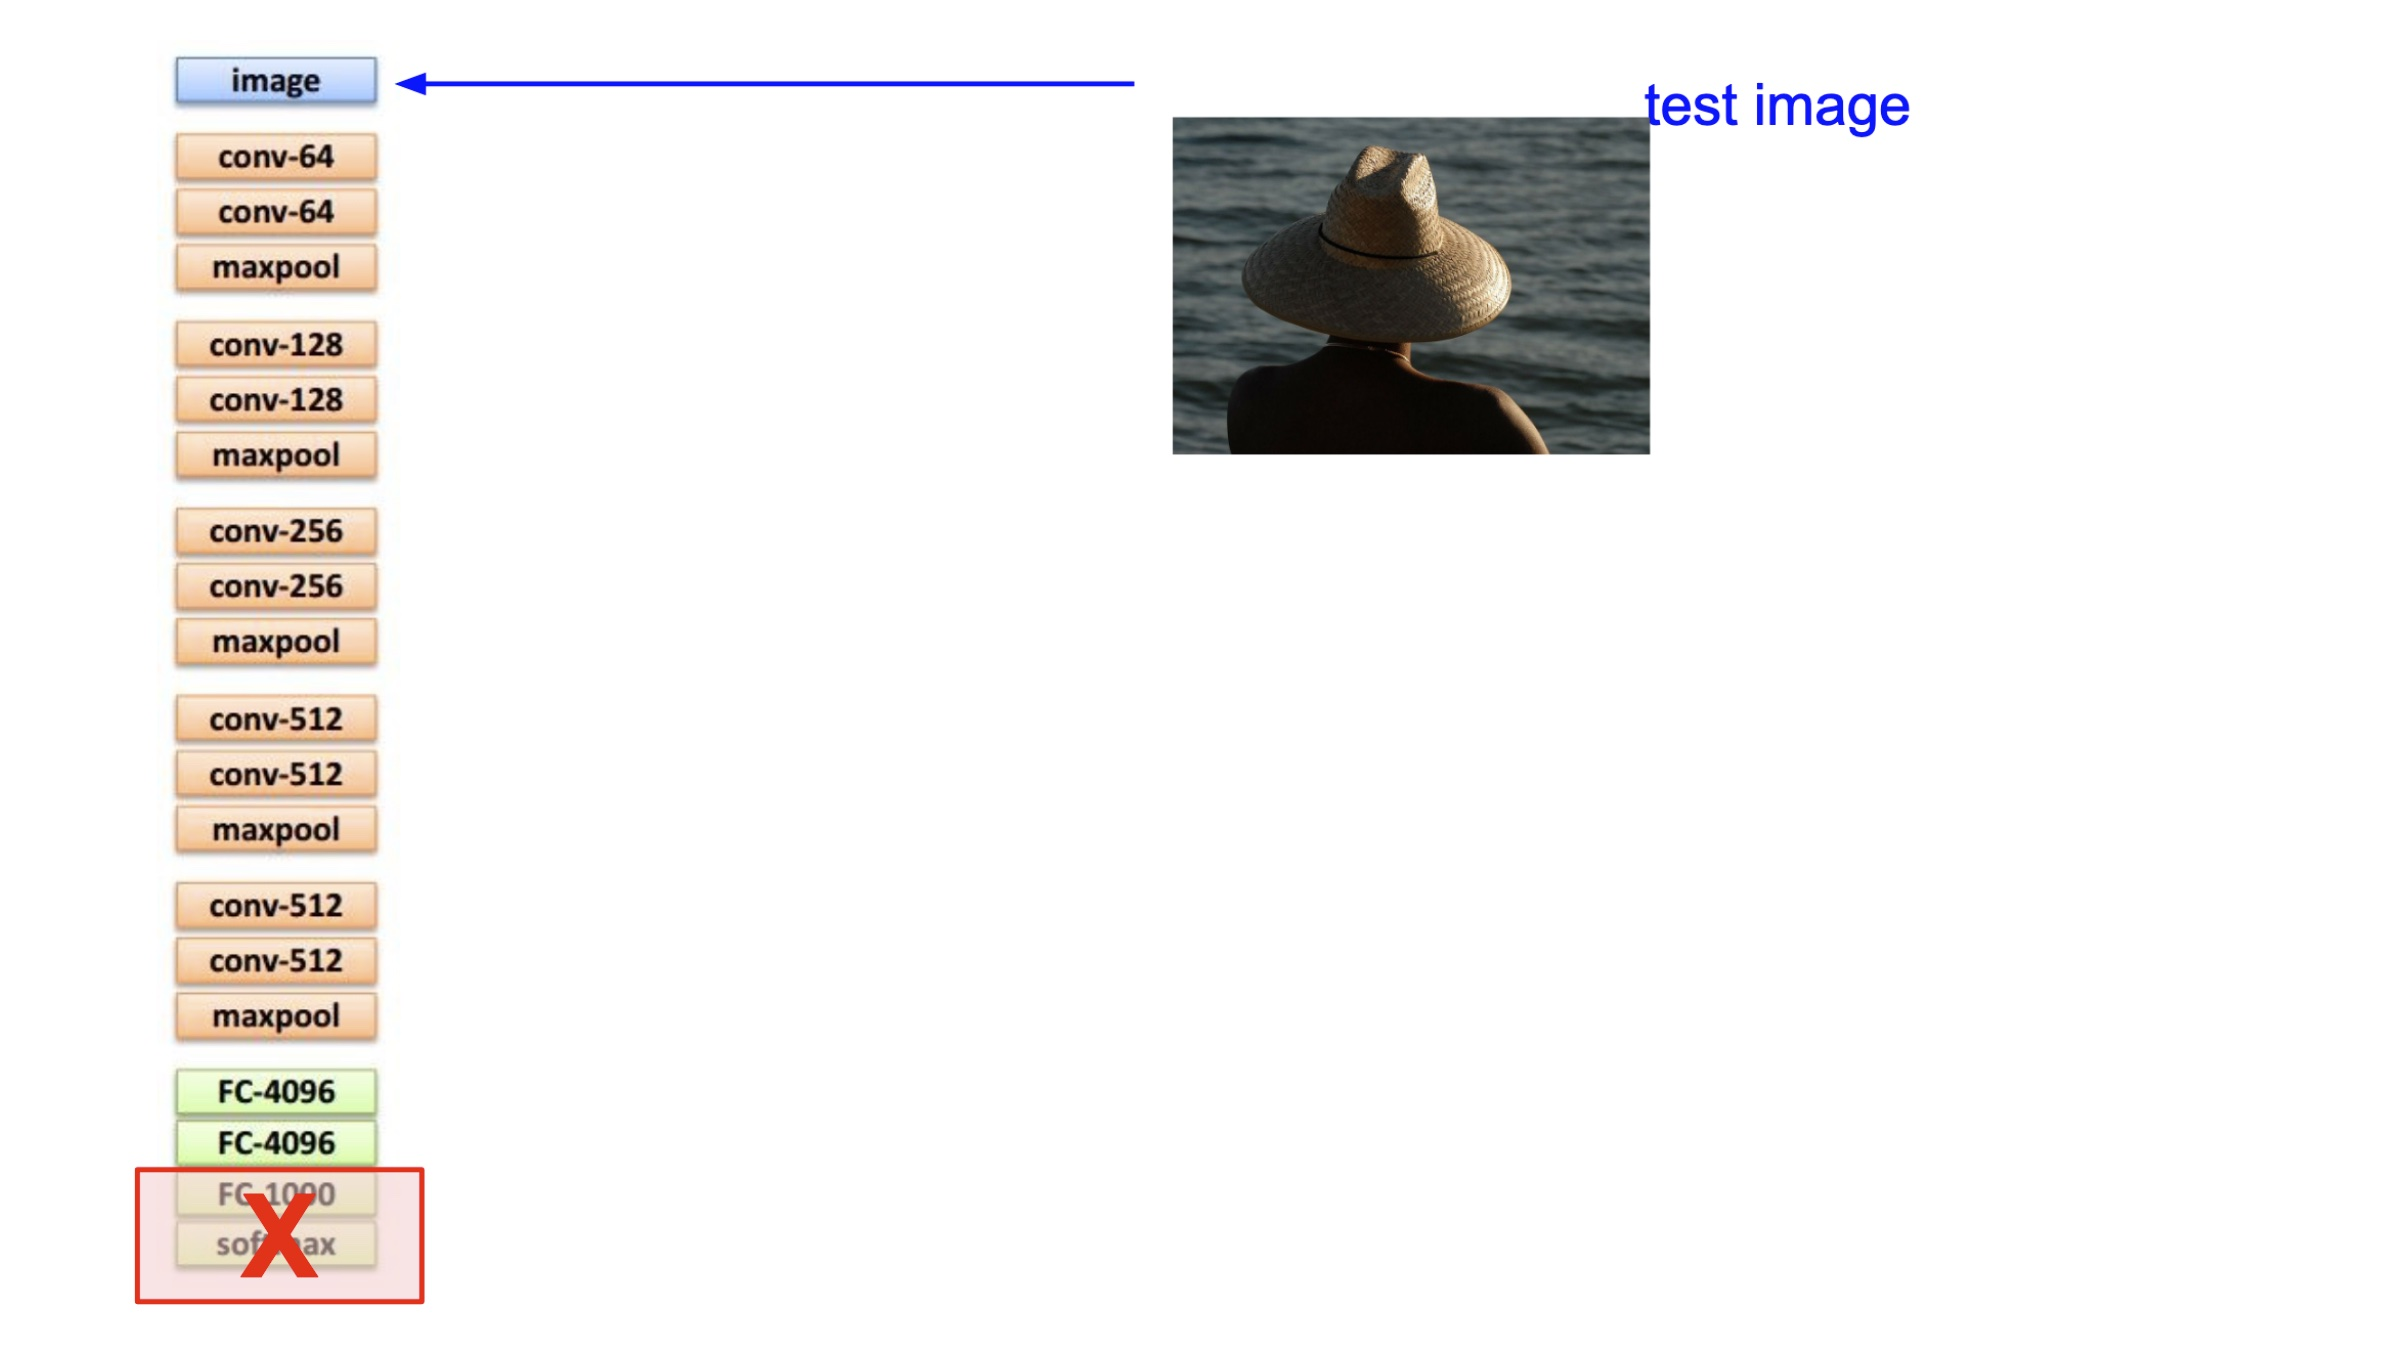
\includegraphics[width=.9\textwidth]{pics/cap3}
\end{center}
\end{frame}


\begin{frame}
\frametitle{Image Captioning: how do we do it?}
\begin{center}
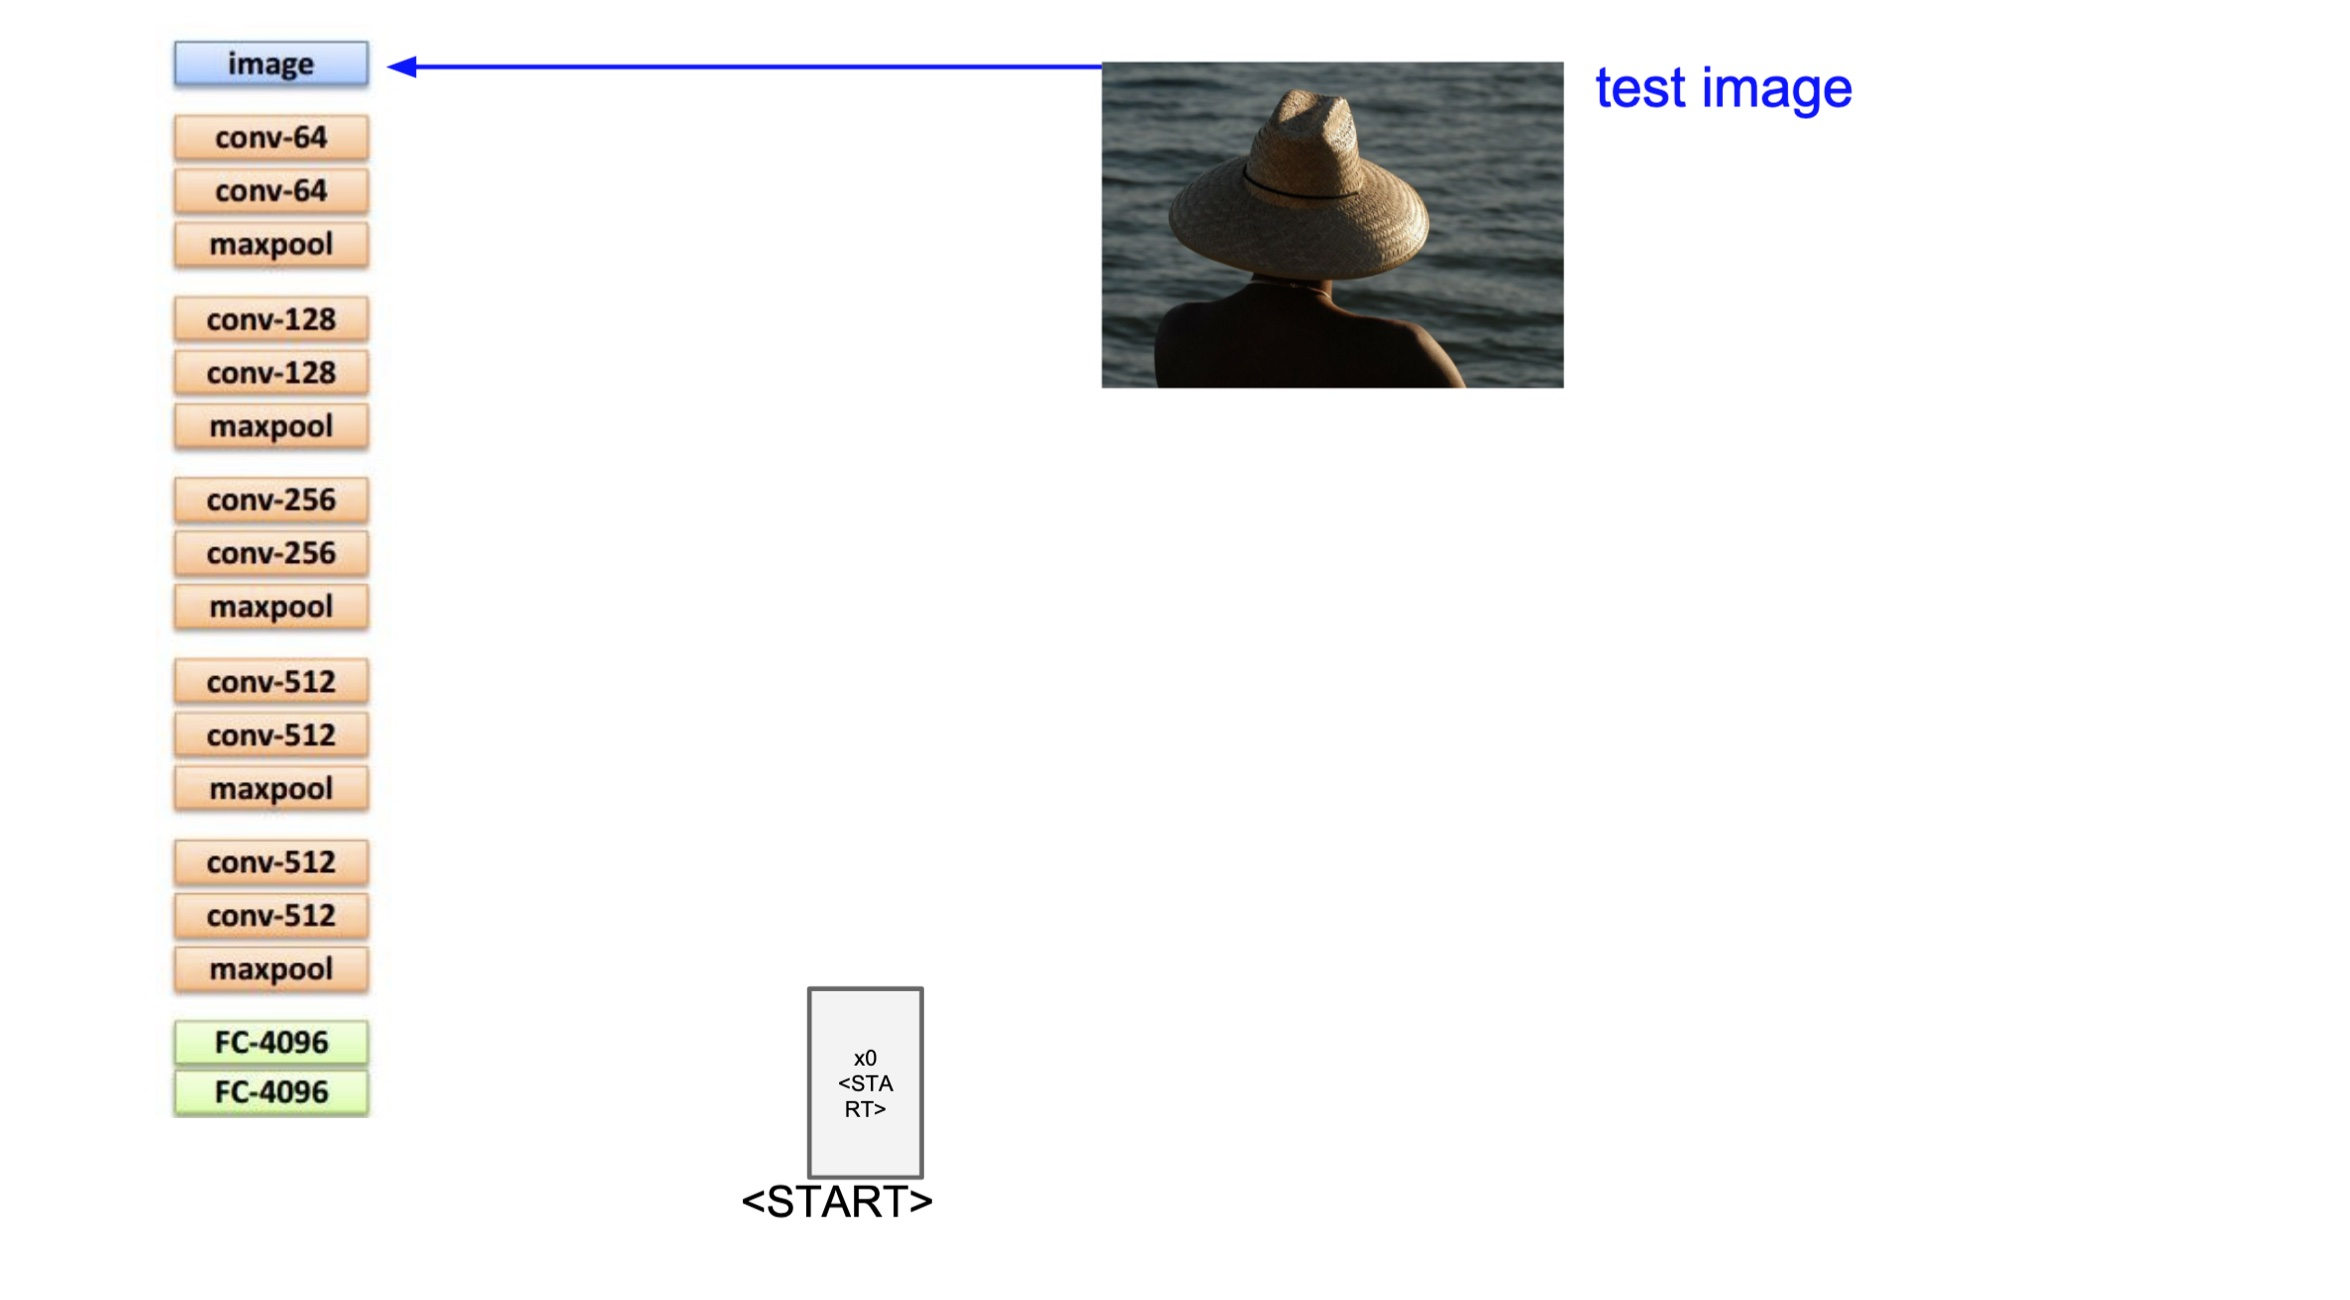
\includegraphics[width=.9\textwidth]{pics/cap4}
\end{center}
\end{frame}

\begin{frame}
\frametitle{Image Captioning: how do we do it?}
\begin{center}
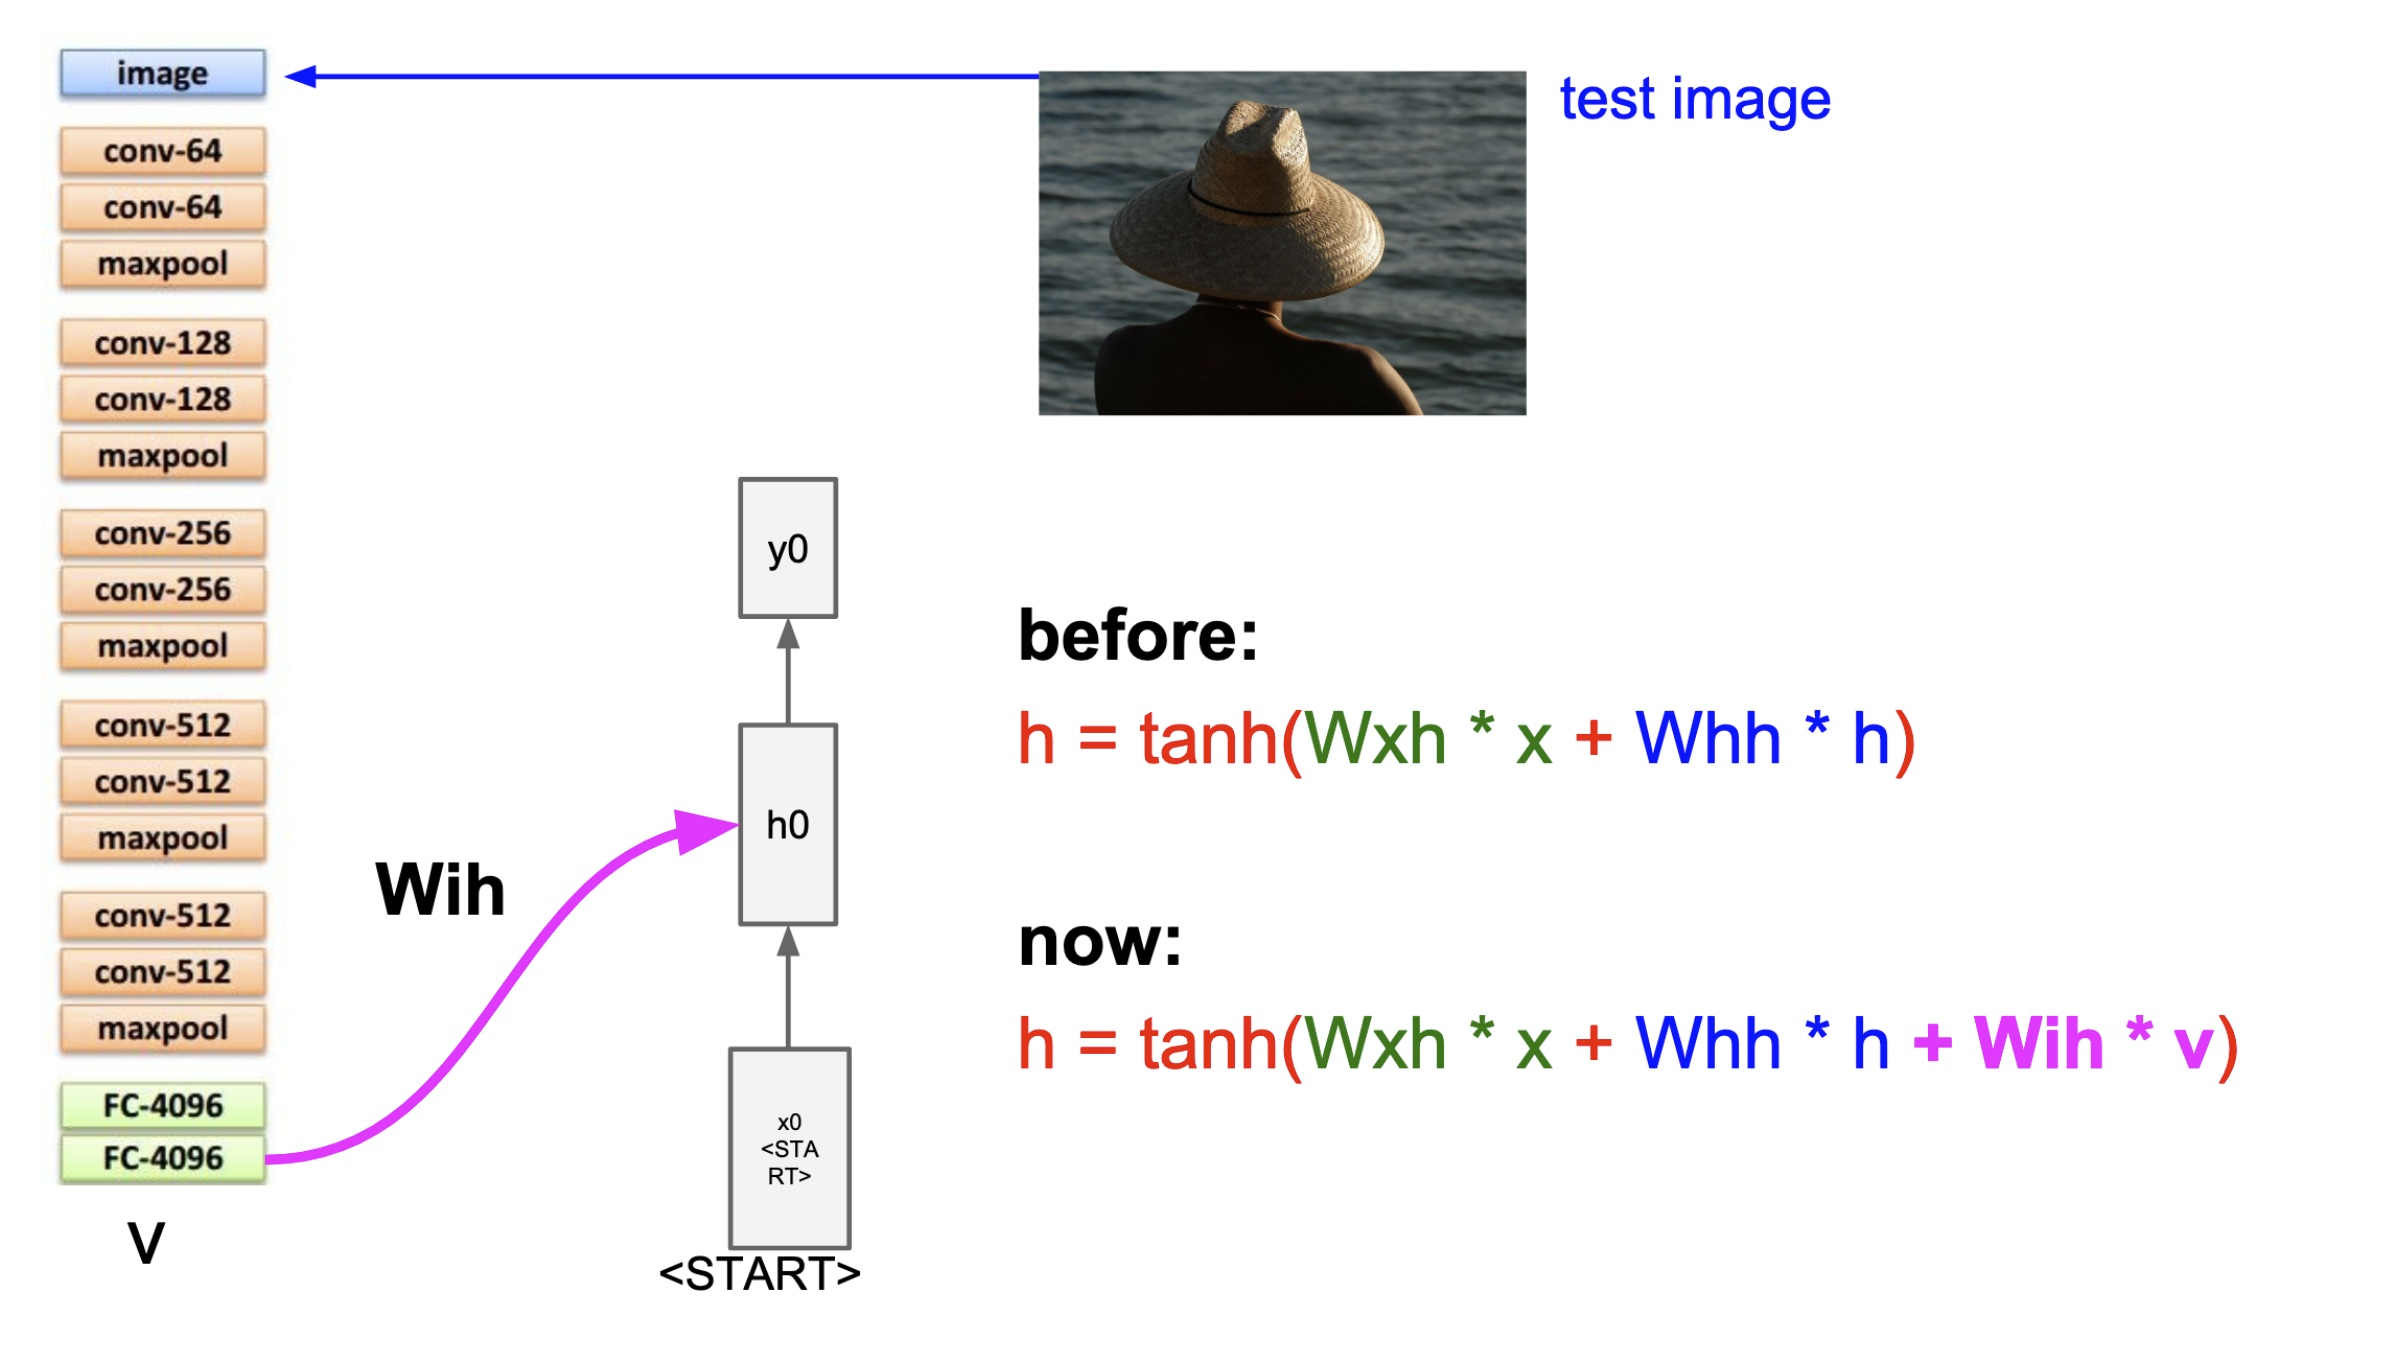
\includegraphics[width=.9\textwidth]{pics/cap5}
\end{center}
\end{frame}

\begin{frame}
\frametitle{Image Captioning: how do we do it?}
\begin{center}
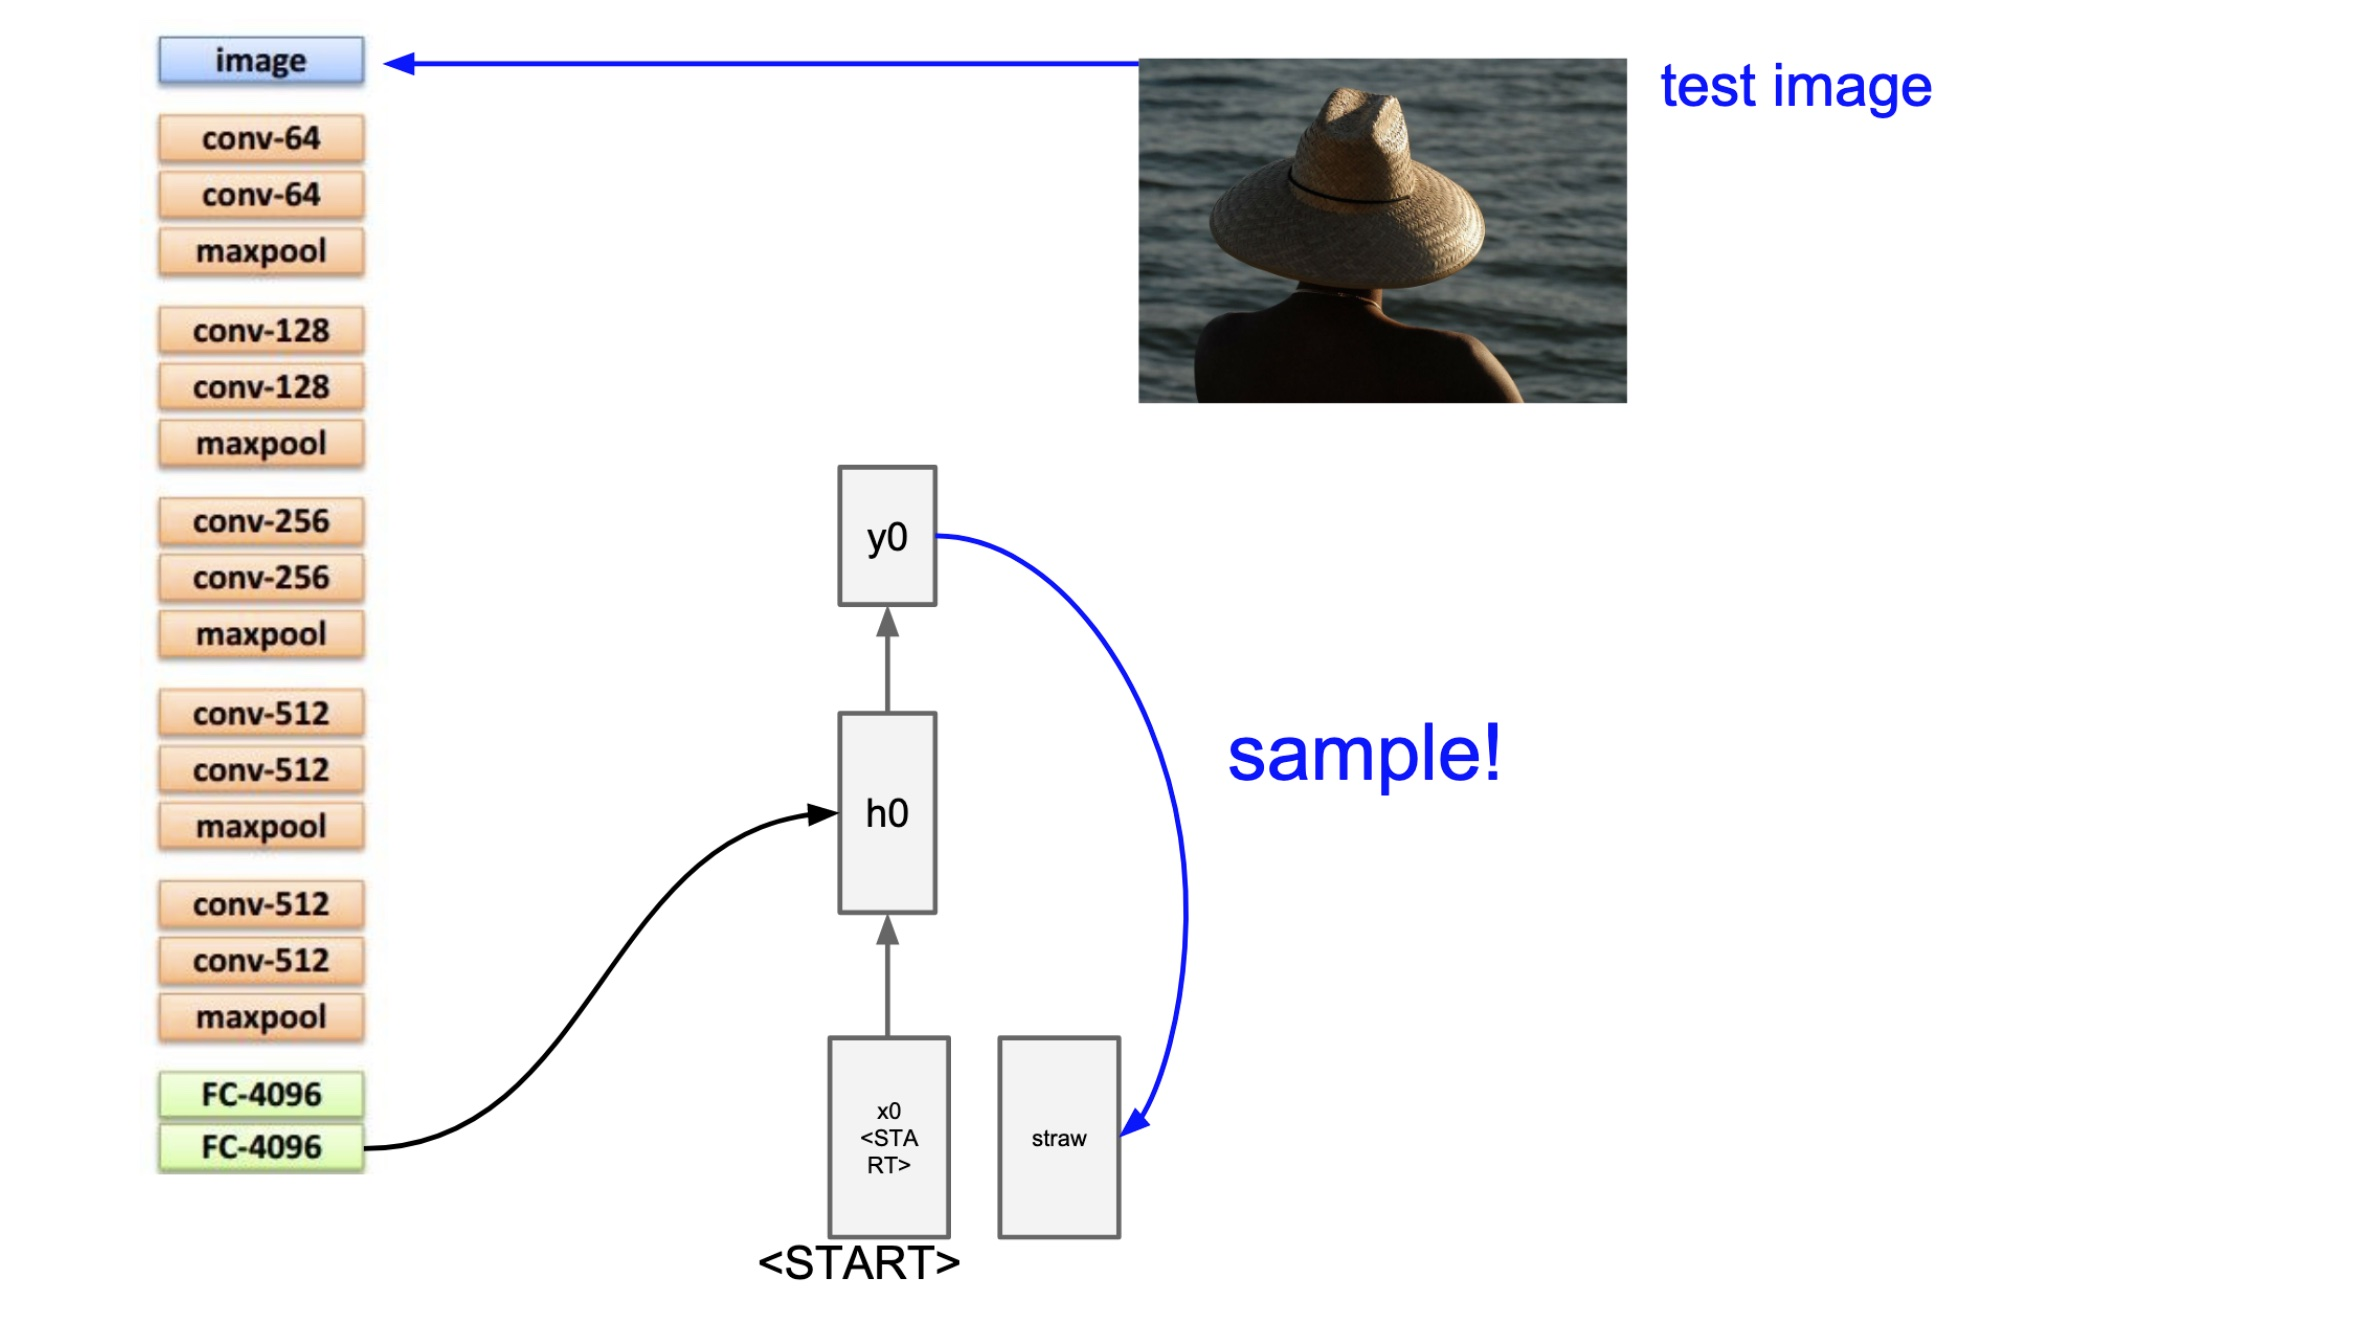
\includegraphics[width=.9\textwidth]{pics/cap6}
\end{center}
\end{frame}

\begin{frame}
\frametitle{Image Captioning: how do we do it?}
\begin{center}
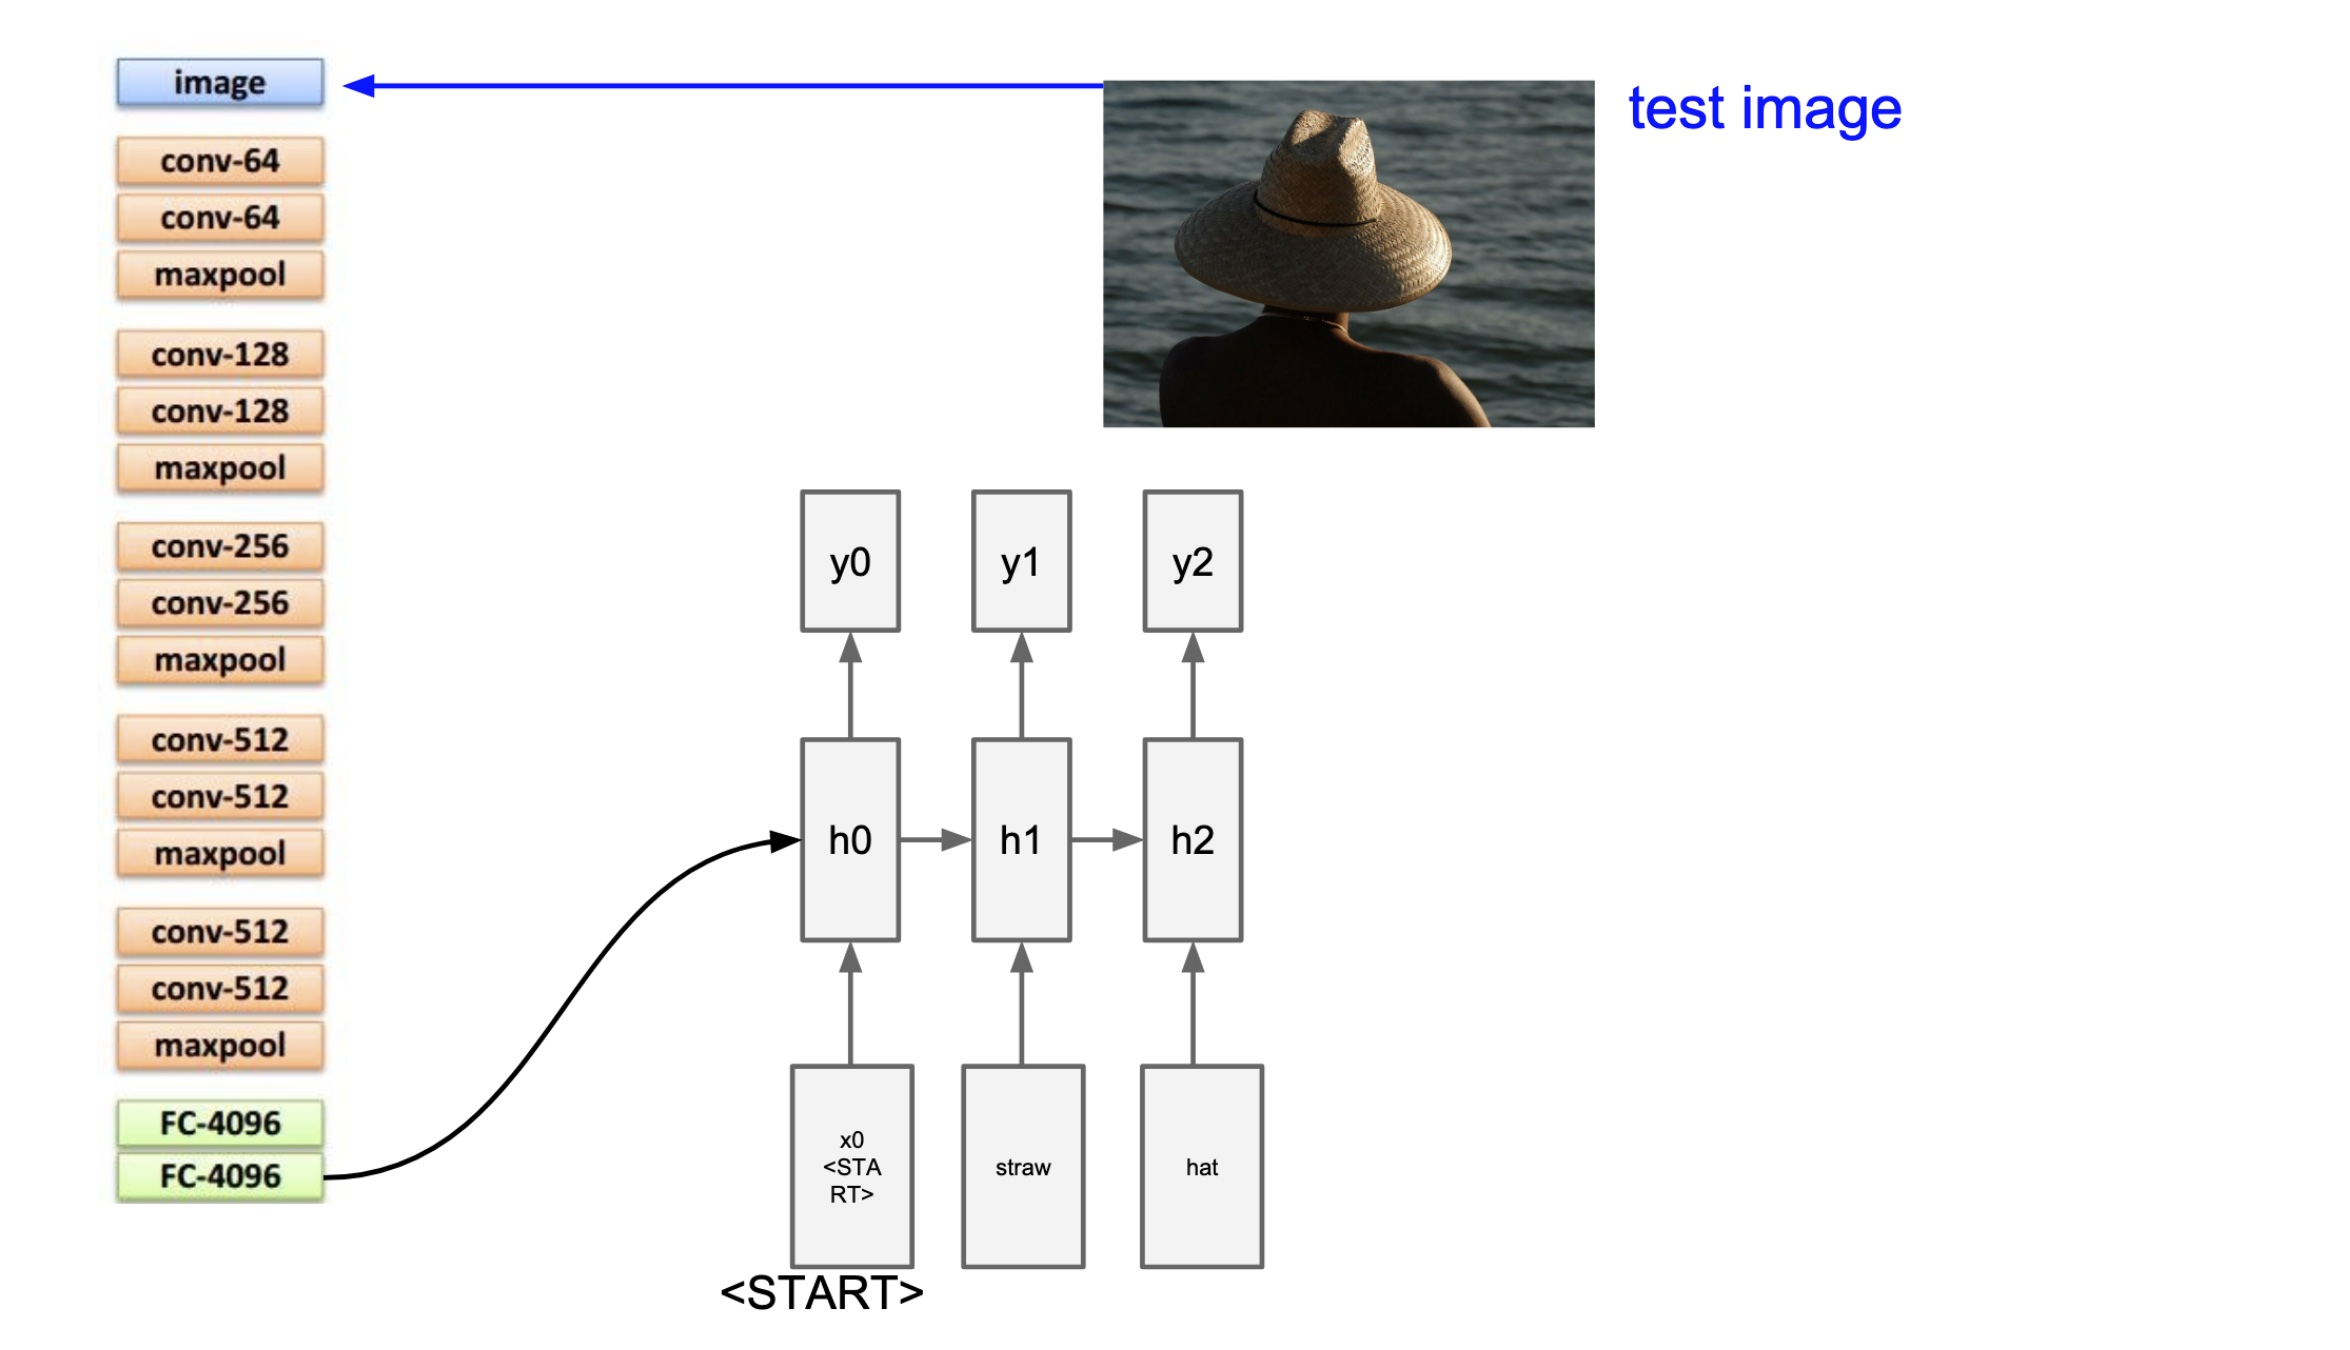
\includegraphics[width=.9\textwidth]{pics/cap7}
\end{center}
\end{frame}

\begin{frame}
\frametitle{Image Captioning: how do we do it?}
\begin{center}
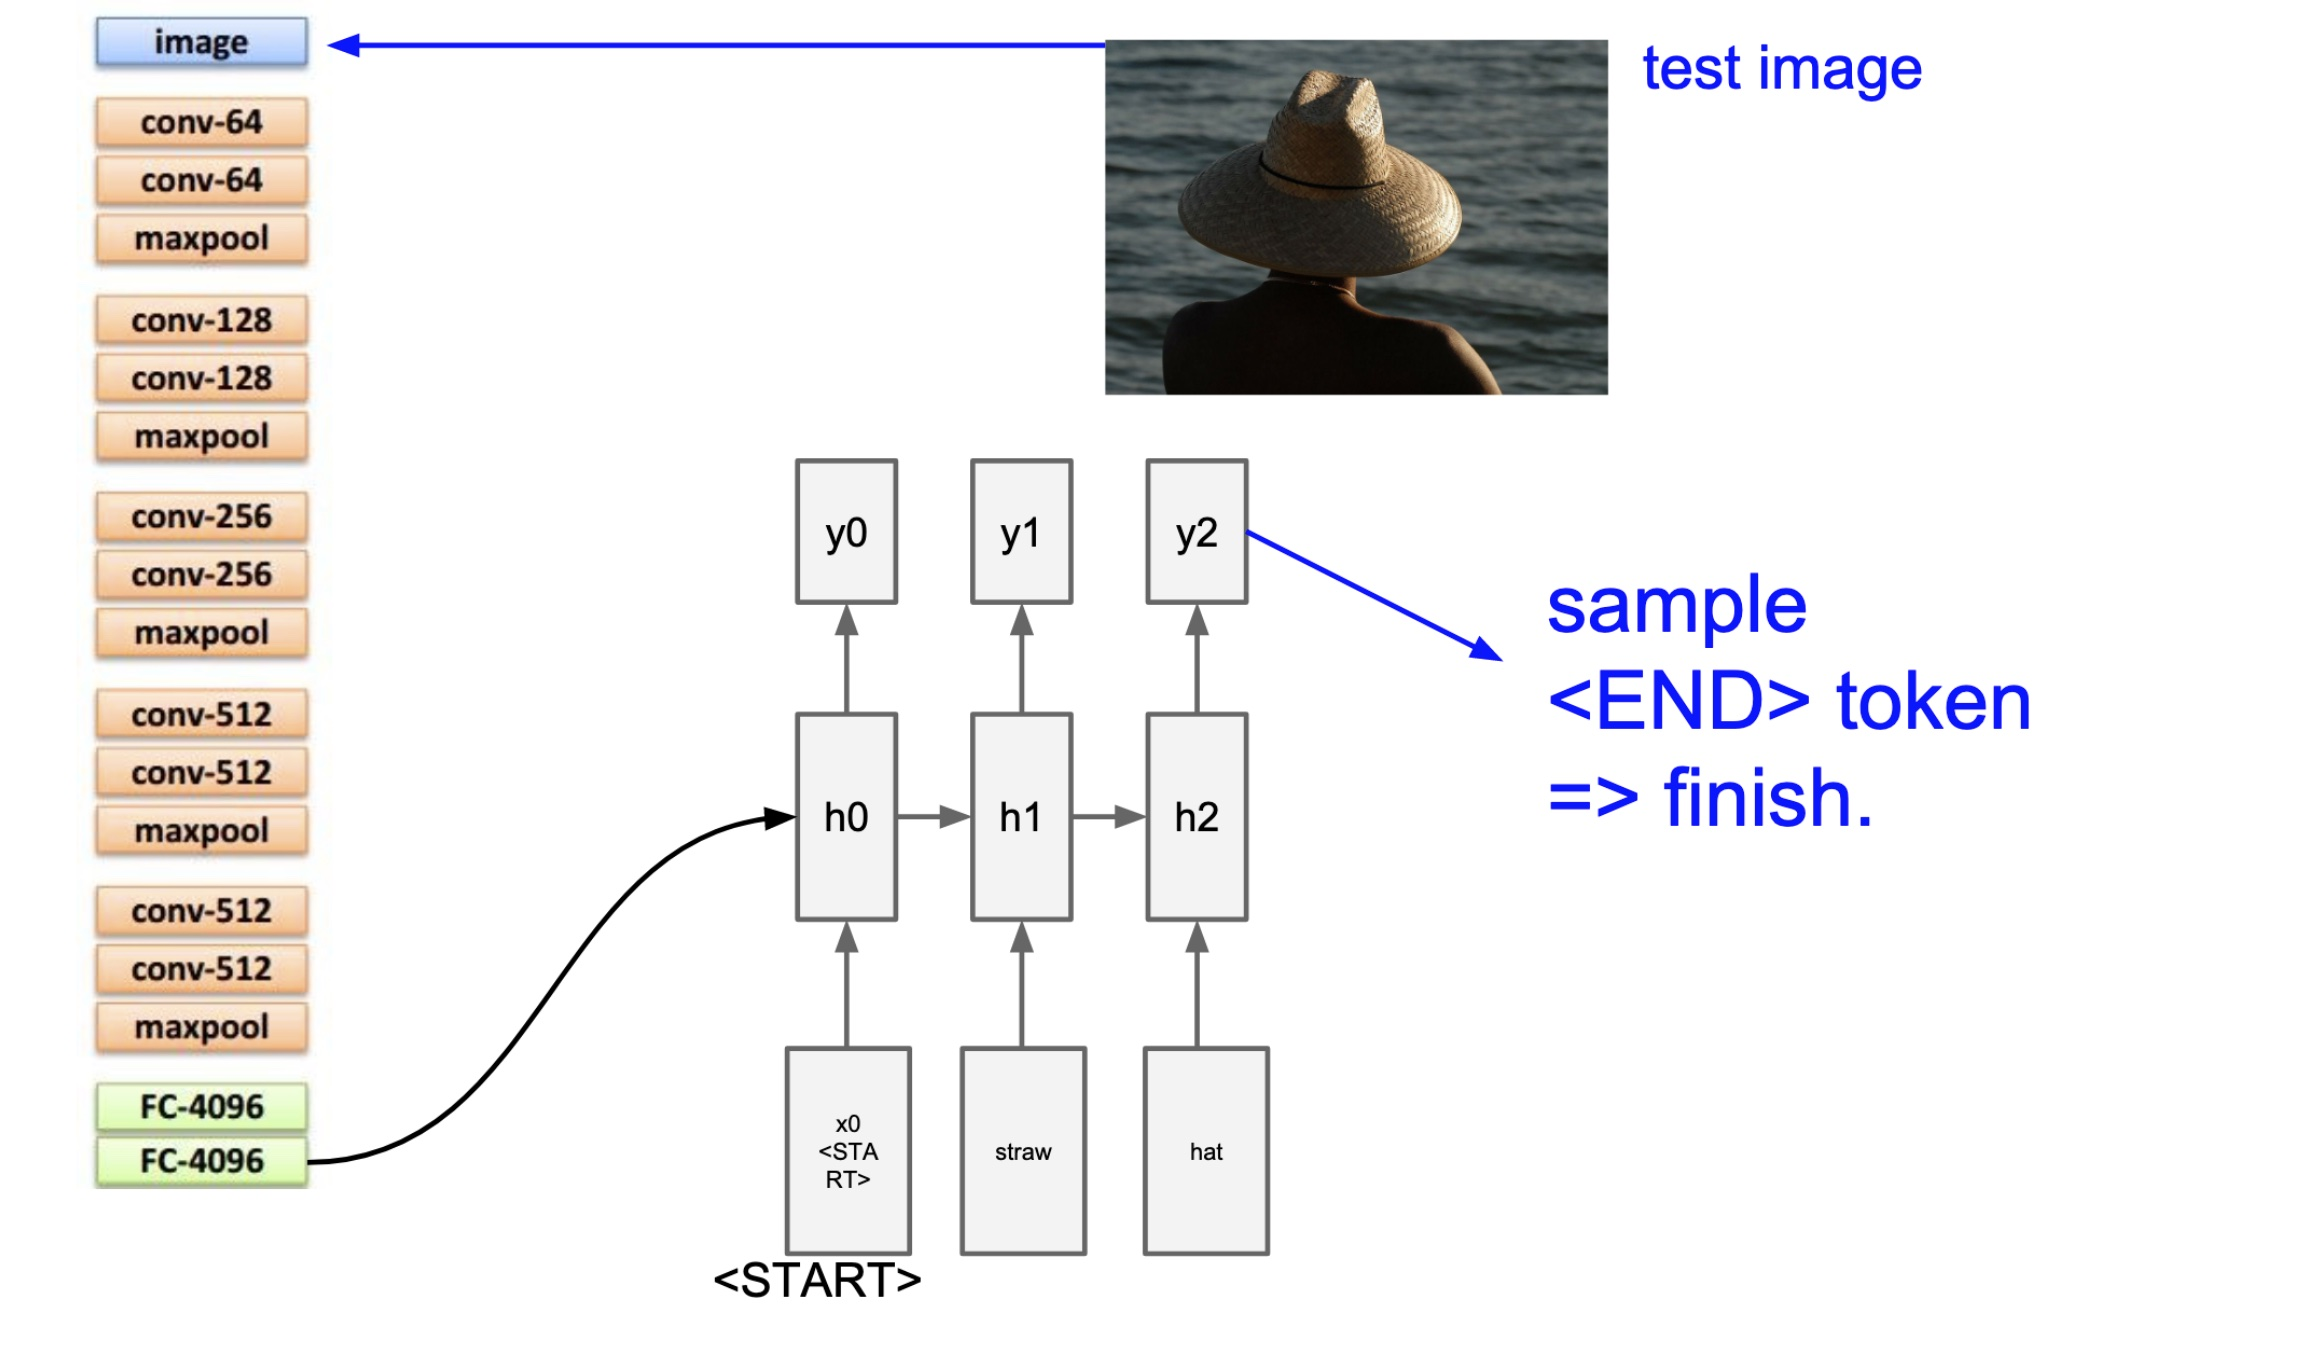
\includegraphics[width=.9\textwidth]{pics/cap8}
\end{center}
\end{frame}

\begin{frame}
\frametitle{Image Captioning: good examples}
\begin{center}
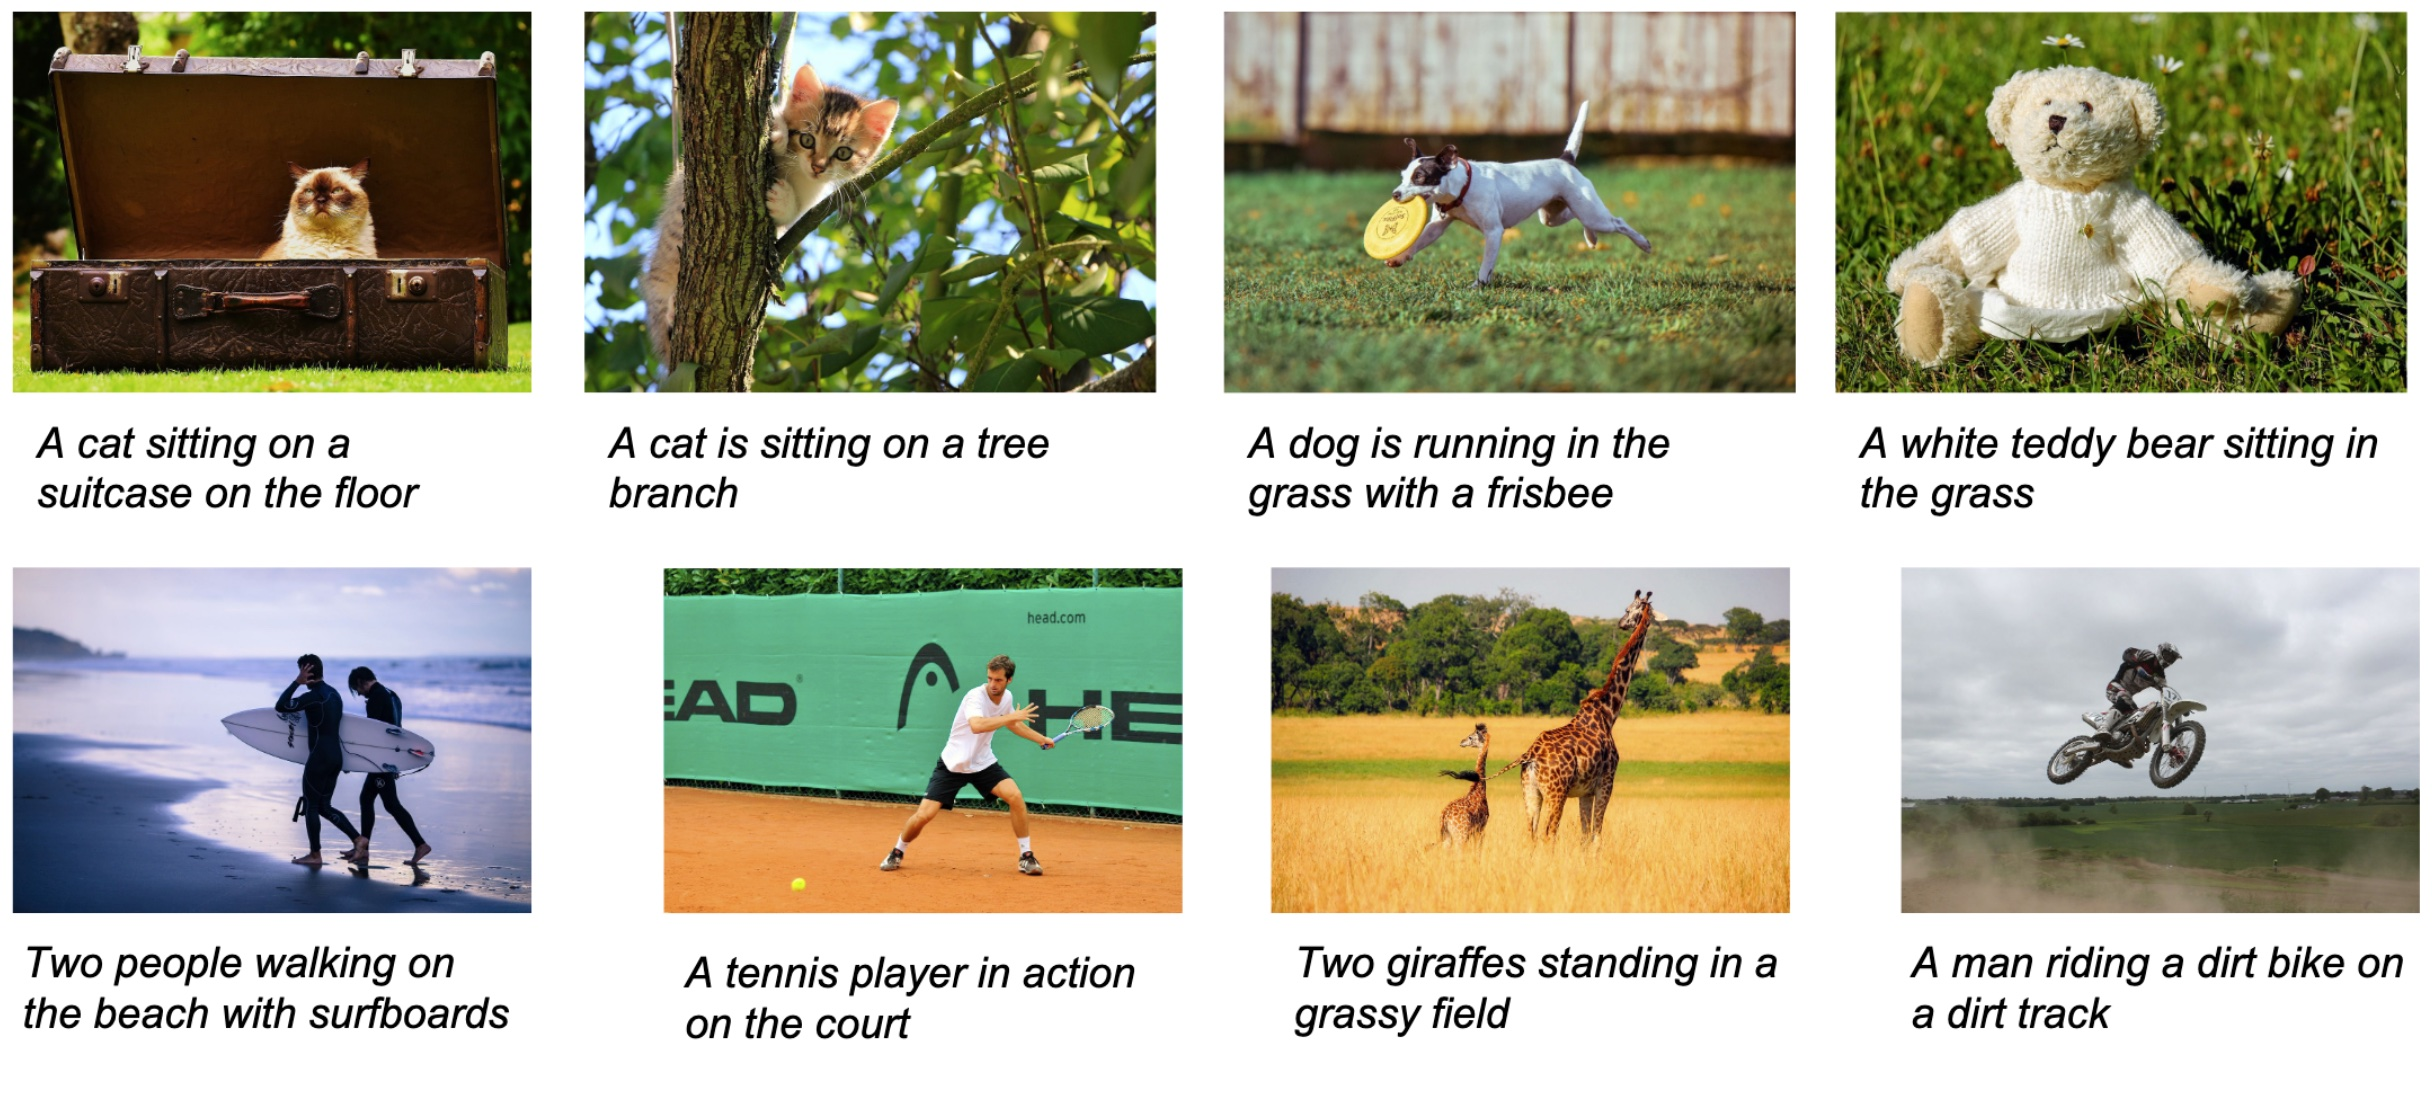
\includegraphics[width=.9\textwidth]{pics/cap9}
\end{center}
\end{frame}

\begin{frame}
\frametitle{Image Captioning: bad examples}
\begin{center}
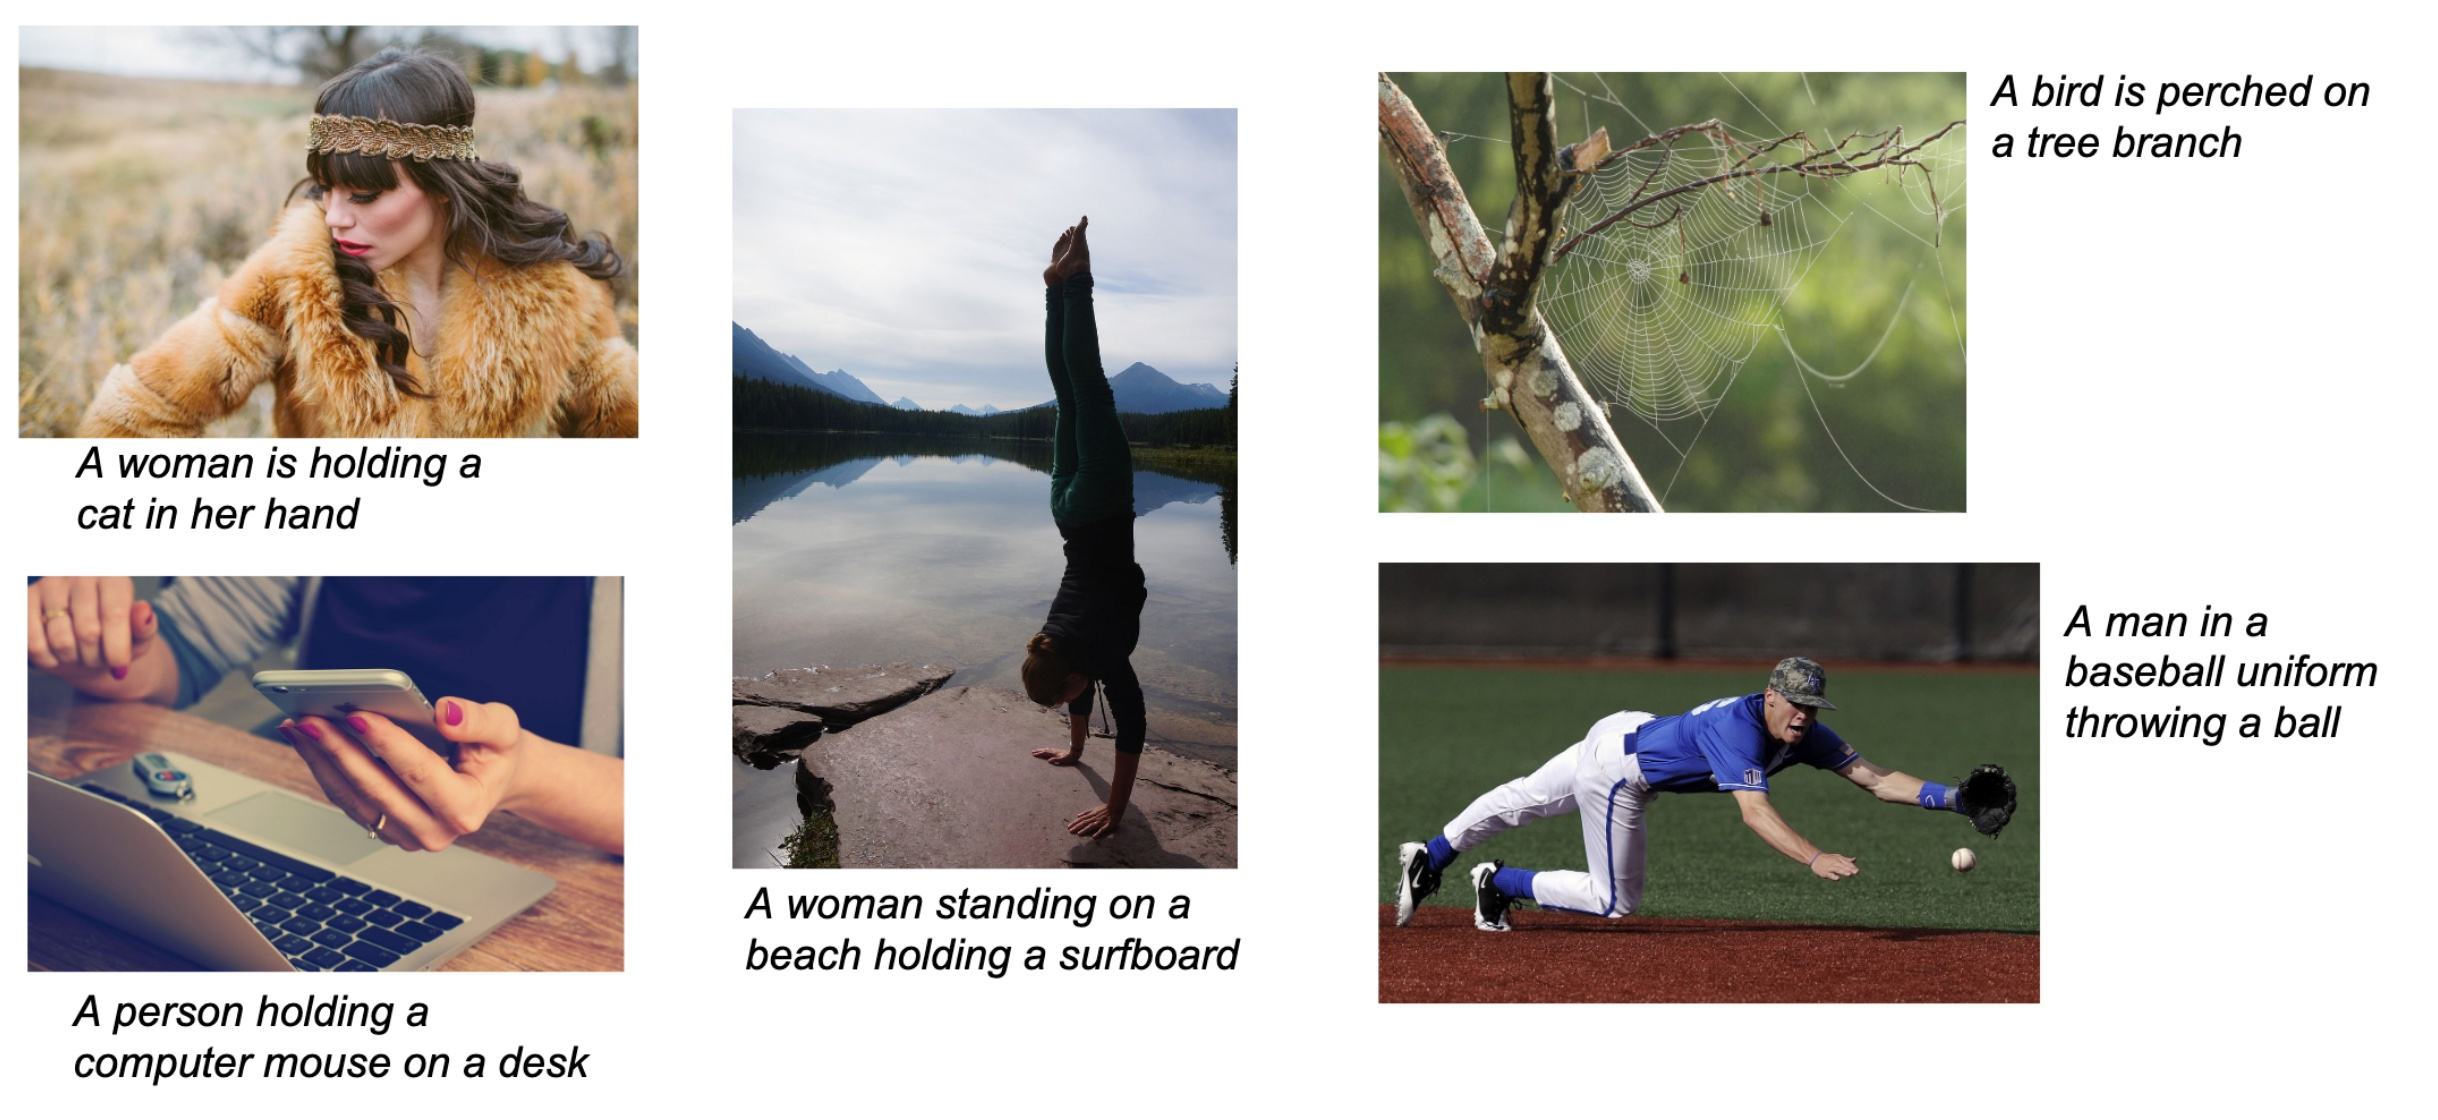
\includegraphics[width=.9\textwidth]{pics/cap10}
\end{center}
\end{frame}

\begin{frame}
\frametitle{Why would the model make such mistakes?}
\begin{center}
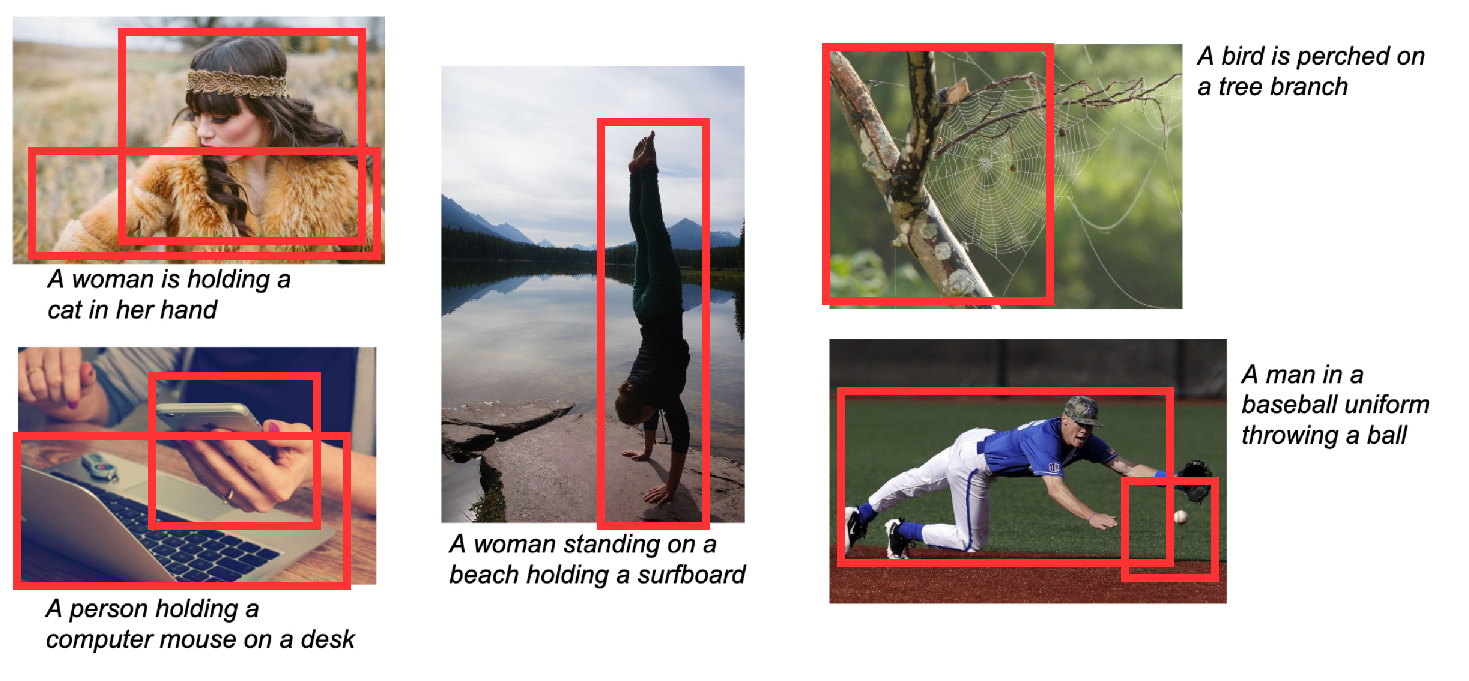
\includegraphics[width=.85\textwidth]{pics/cap11}
\end{center}
\pause
\begin{itemize}
	\item frequency of concepts co-occurring together (e.g., computer mouse - computer desk, tree - bird, cat - woman)
	\pause
	\item each image is unique, so \textbf{more focus on important parts of the image} might help the model to correctly describe the image
\end{itemize}
\end{frame}

\begin{frame}
\frametitle{Image Captioning with Attention \citep{xu2016show}}
\begin{center}
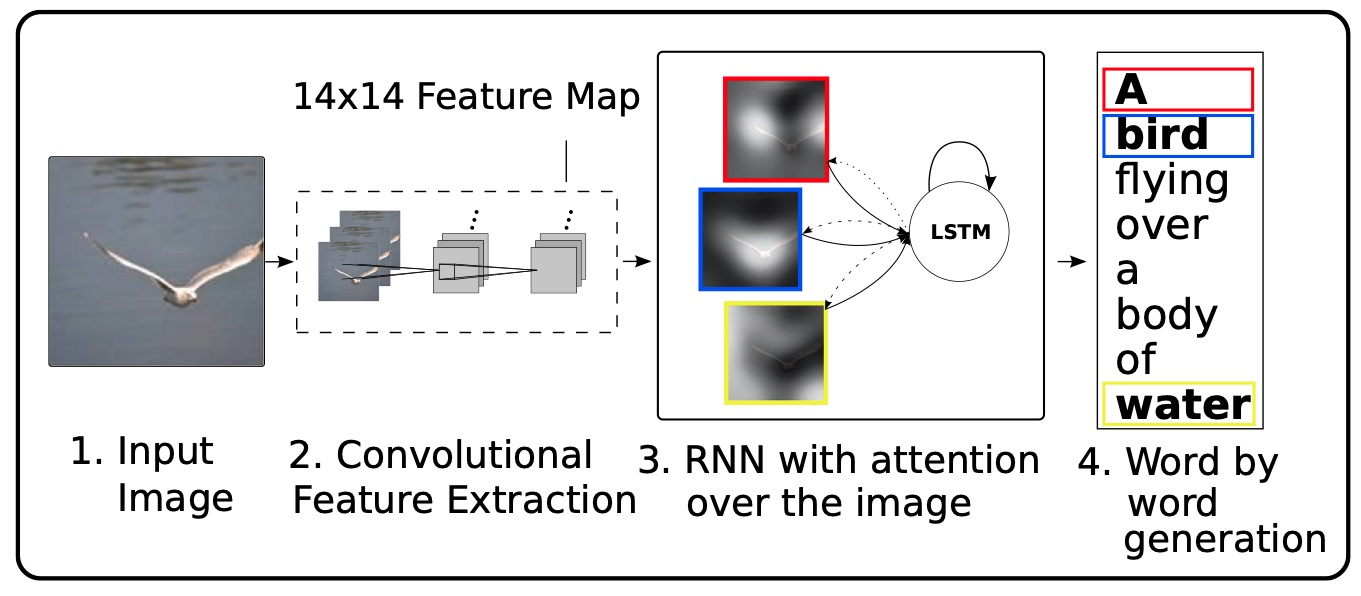
\includegraphics[width=.9\textwidth]{pics/att1}
\end{center}
\end{frame}

\begin{frame}
\frametitle{Why do we need attention and what is so interesting about it?}

\begin{itemize}
	\item prior to language-and-vision tasks, attention has been initially introduced in the domain of machine translation \citep{bahdanau2016neural}
	\pause
	\item the main idea is that \textbf{every word that we say is grounded in the image and we want our model to correctly ground words into objects}
	\pause
	\item it is hard to ground relations (e.g., flying) and both language and vision modalities can be more important for grounding of particular word types \citep{lu2017,ghanimifard2019,ilinykh2021}
	\pause
	\item \textit{project idea sketch}: examine grounding of (spatial) relations in multi-modal set-up
\end{itemize}

\end{frame}


\begin{frame}
\frametitle{Attention in ICM}
\begin{center}
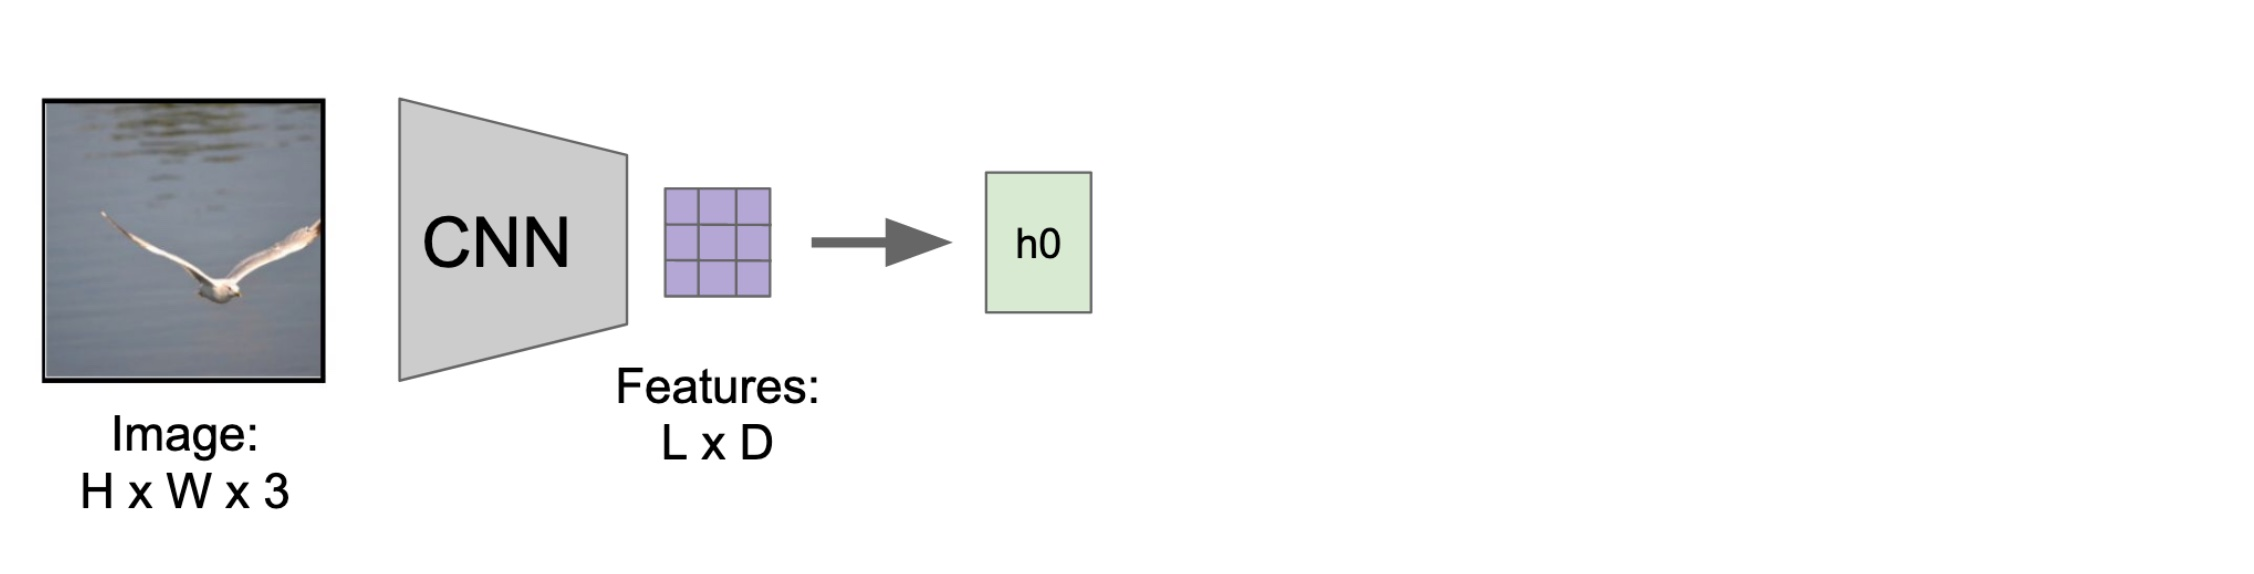
\includegraphics[width=1\textwidth]{pics/att2}
\end{center}
\end{frame}

\begin{frame}
\frametitle{Attention in ICM}
\begin{center}
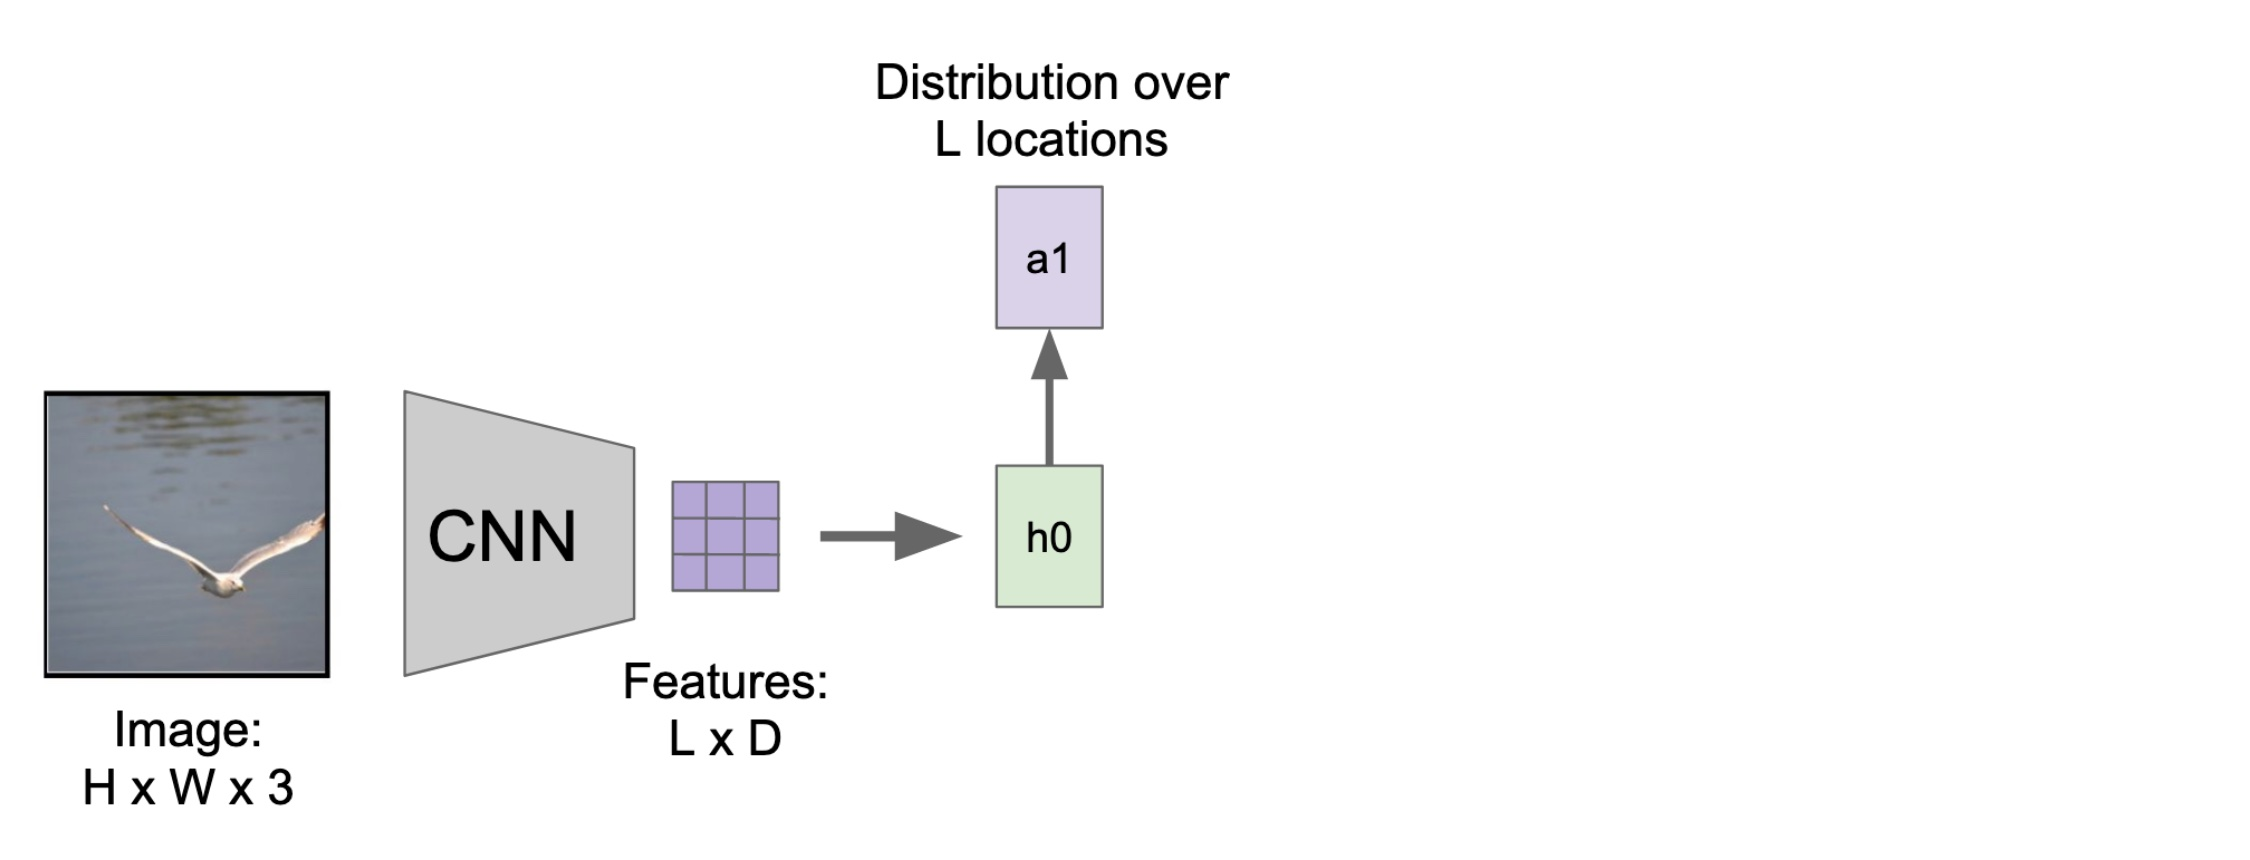
\includegraphics[width=1\textwidth]{pics/att3}
\end{center}
\end{frame}

\begin{frame}
\frametitle{Attention in ICM}
\begin{center}
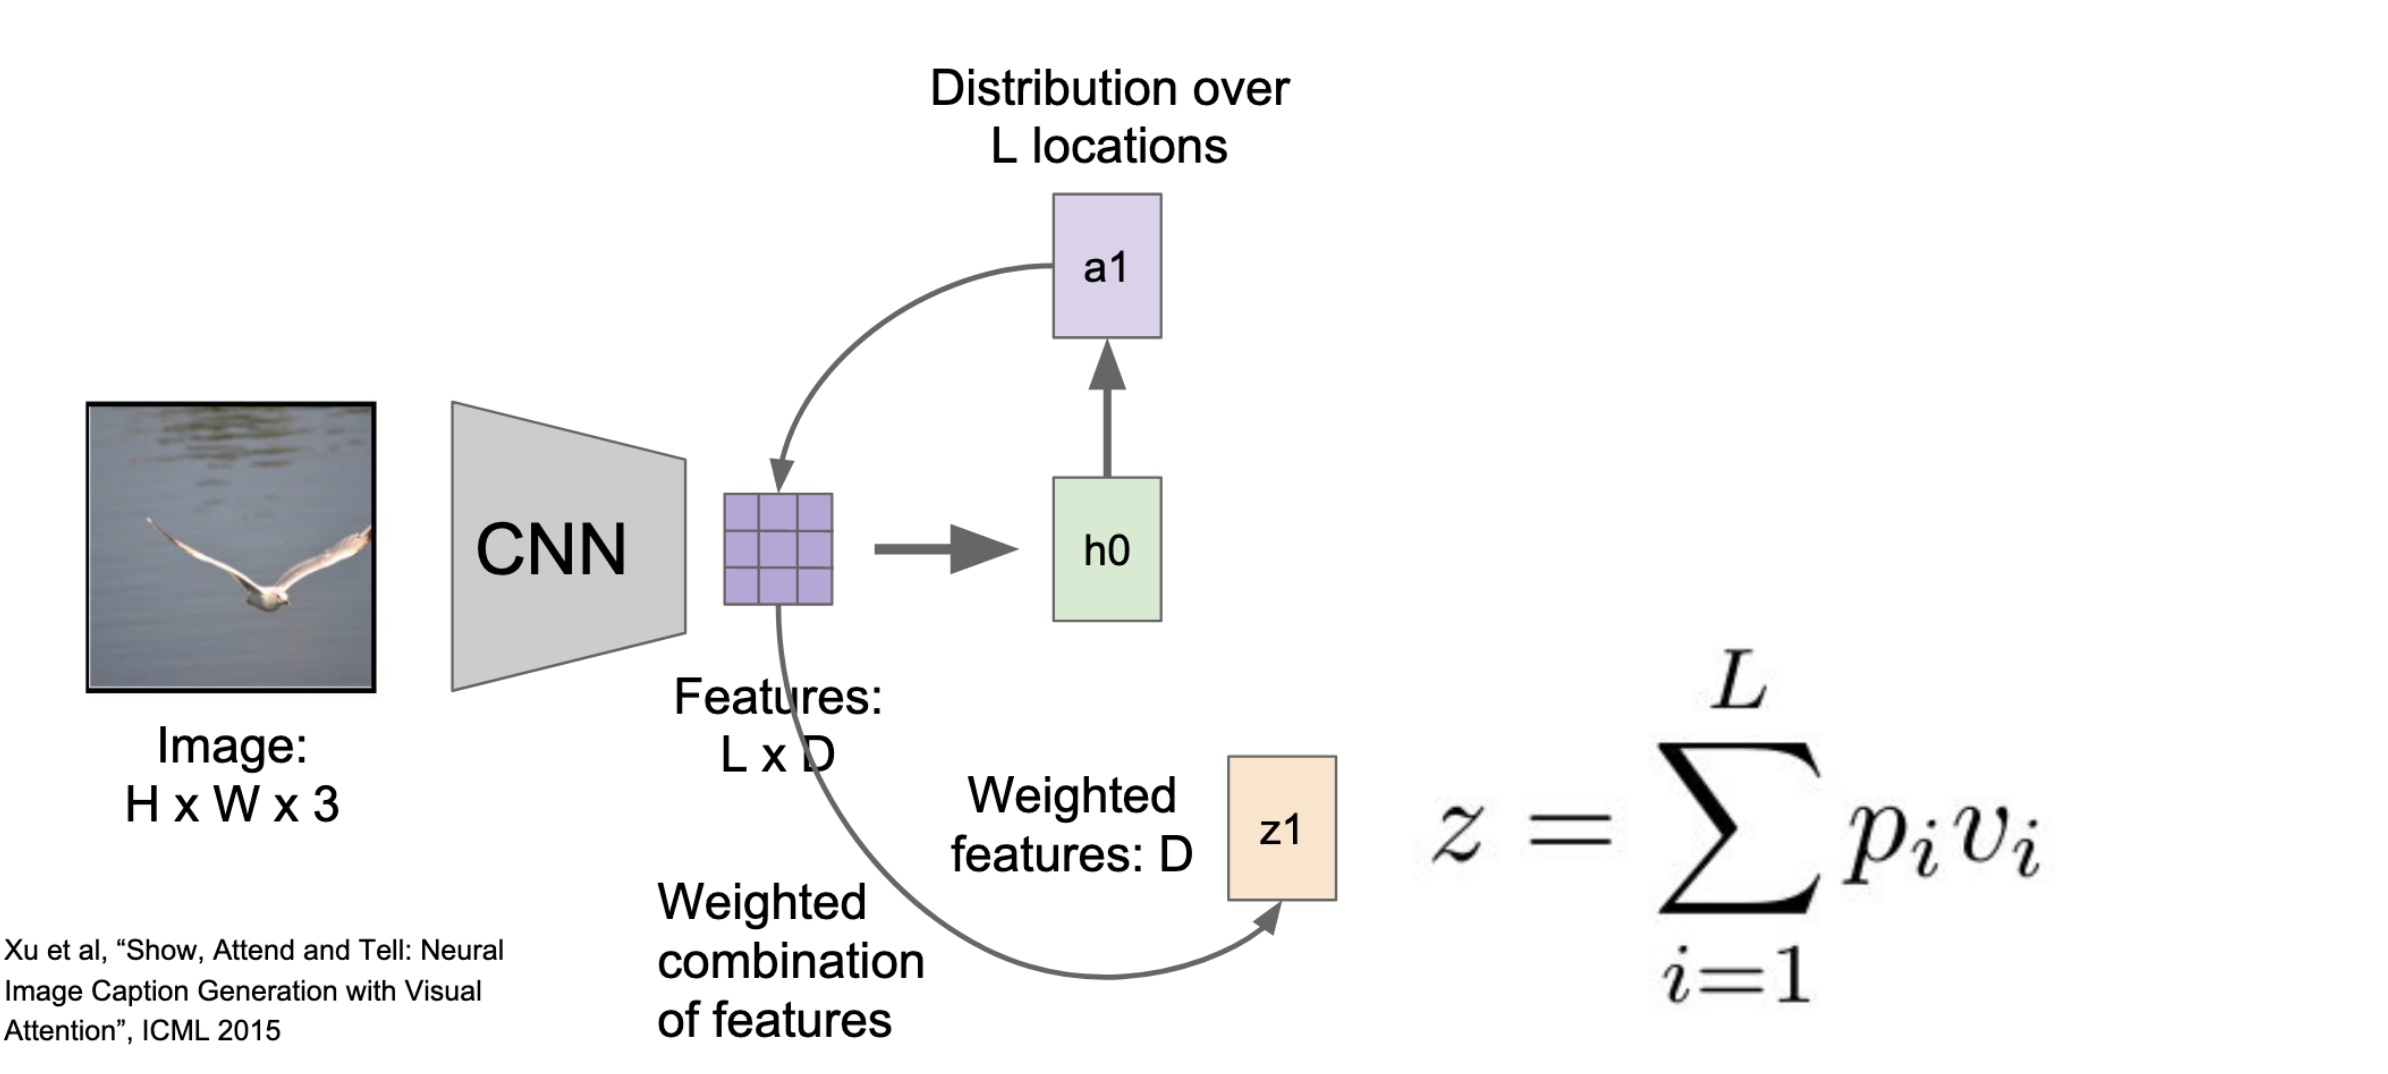
\includegraphics[width=1\textwidth]{pics/att4}
\end{center}
\end{frame}

\begin{frame}
\frametitle{Attention in ICM}
\begin{center}
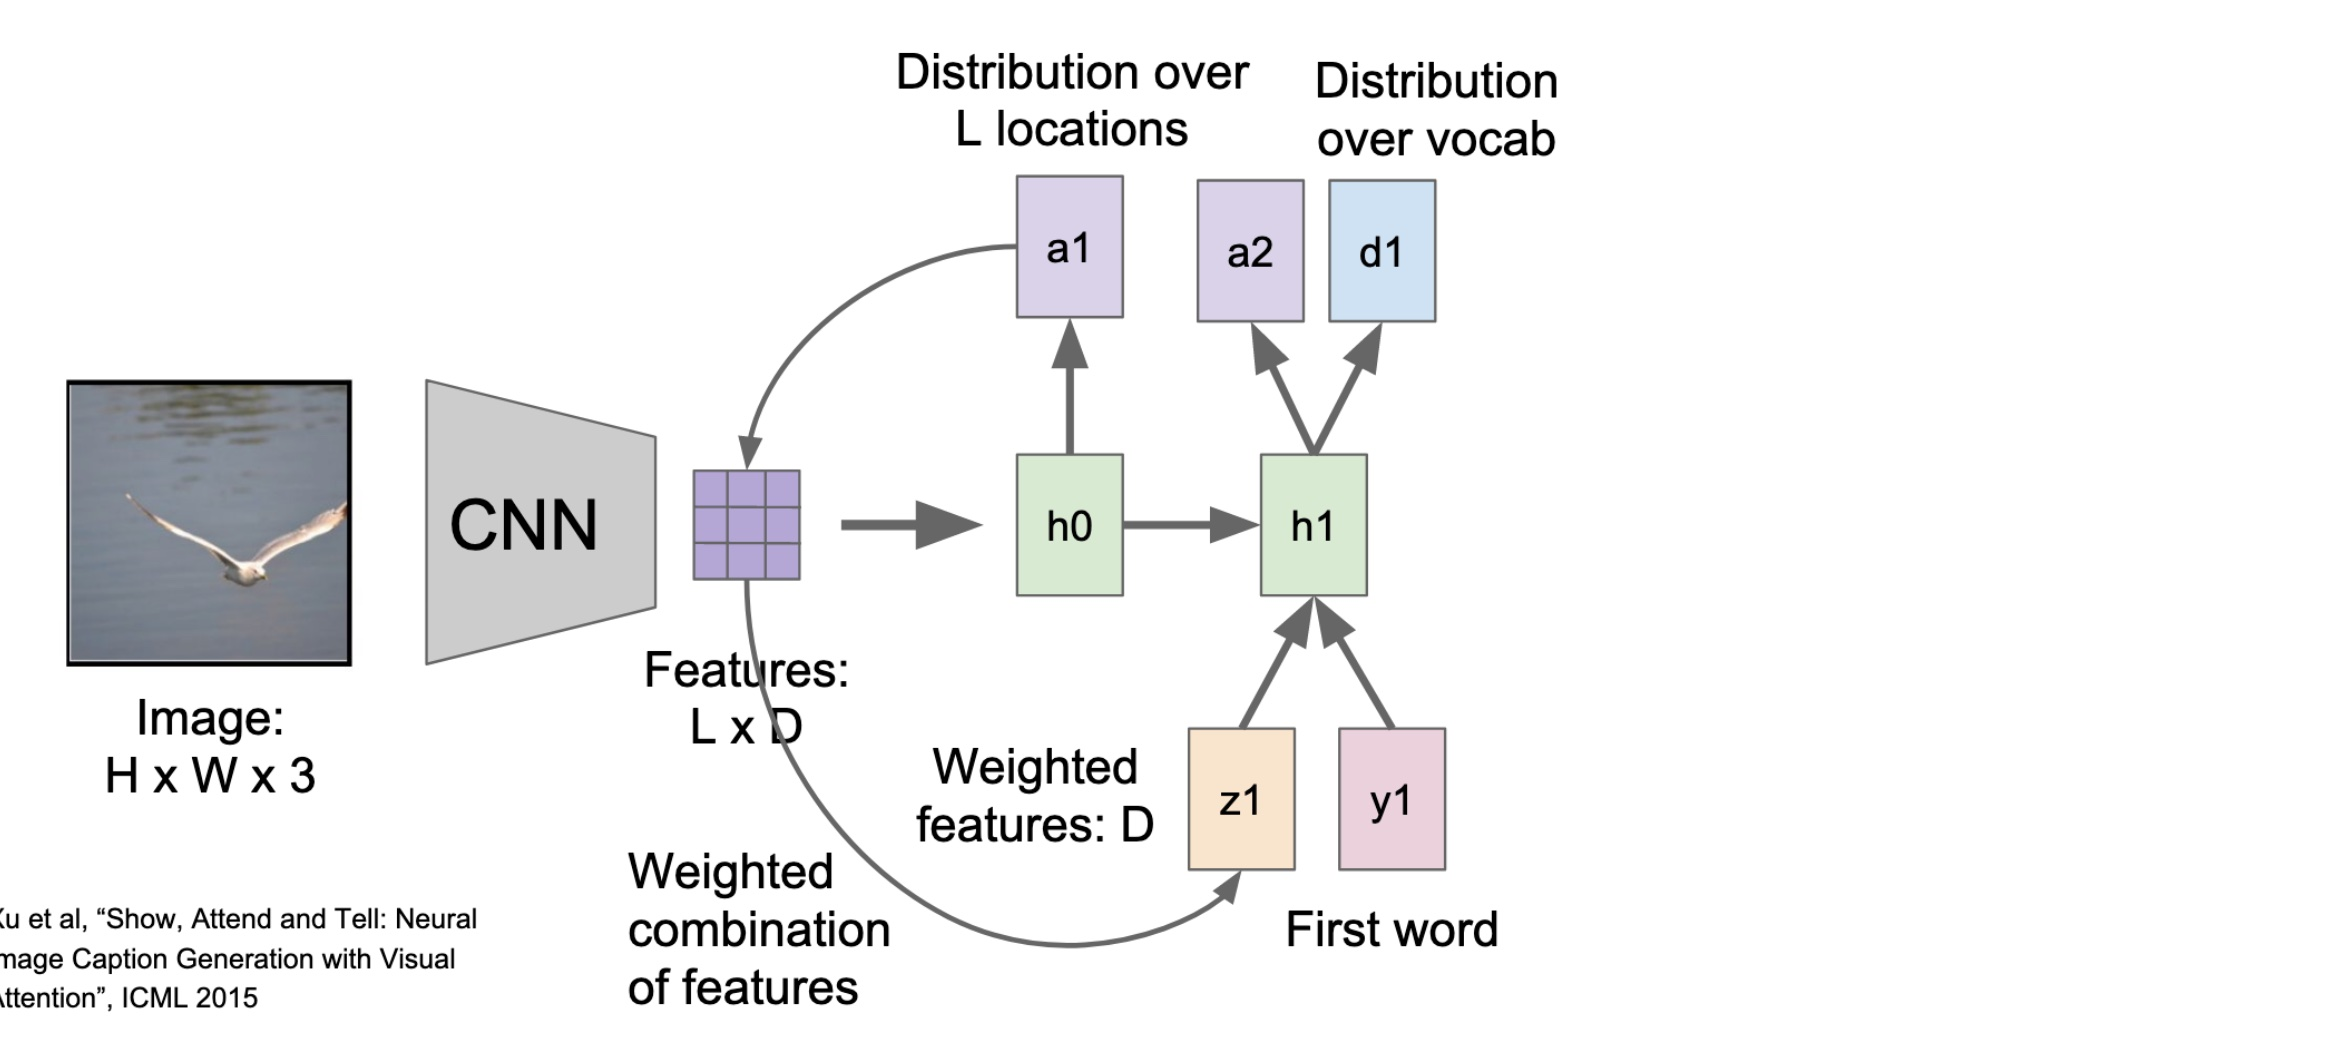
\includegraphics[width=1\textwidth]{pics/att5}
\end{center}
\end{frame}

\begin{frame}
\frametitle{Attention in ICM}
\begin{center}
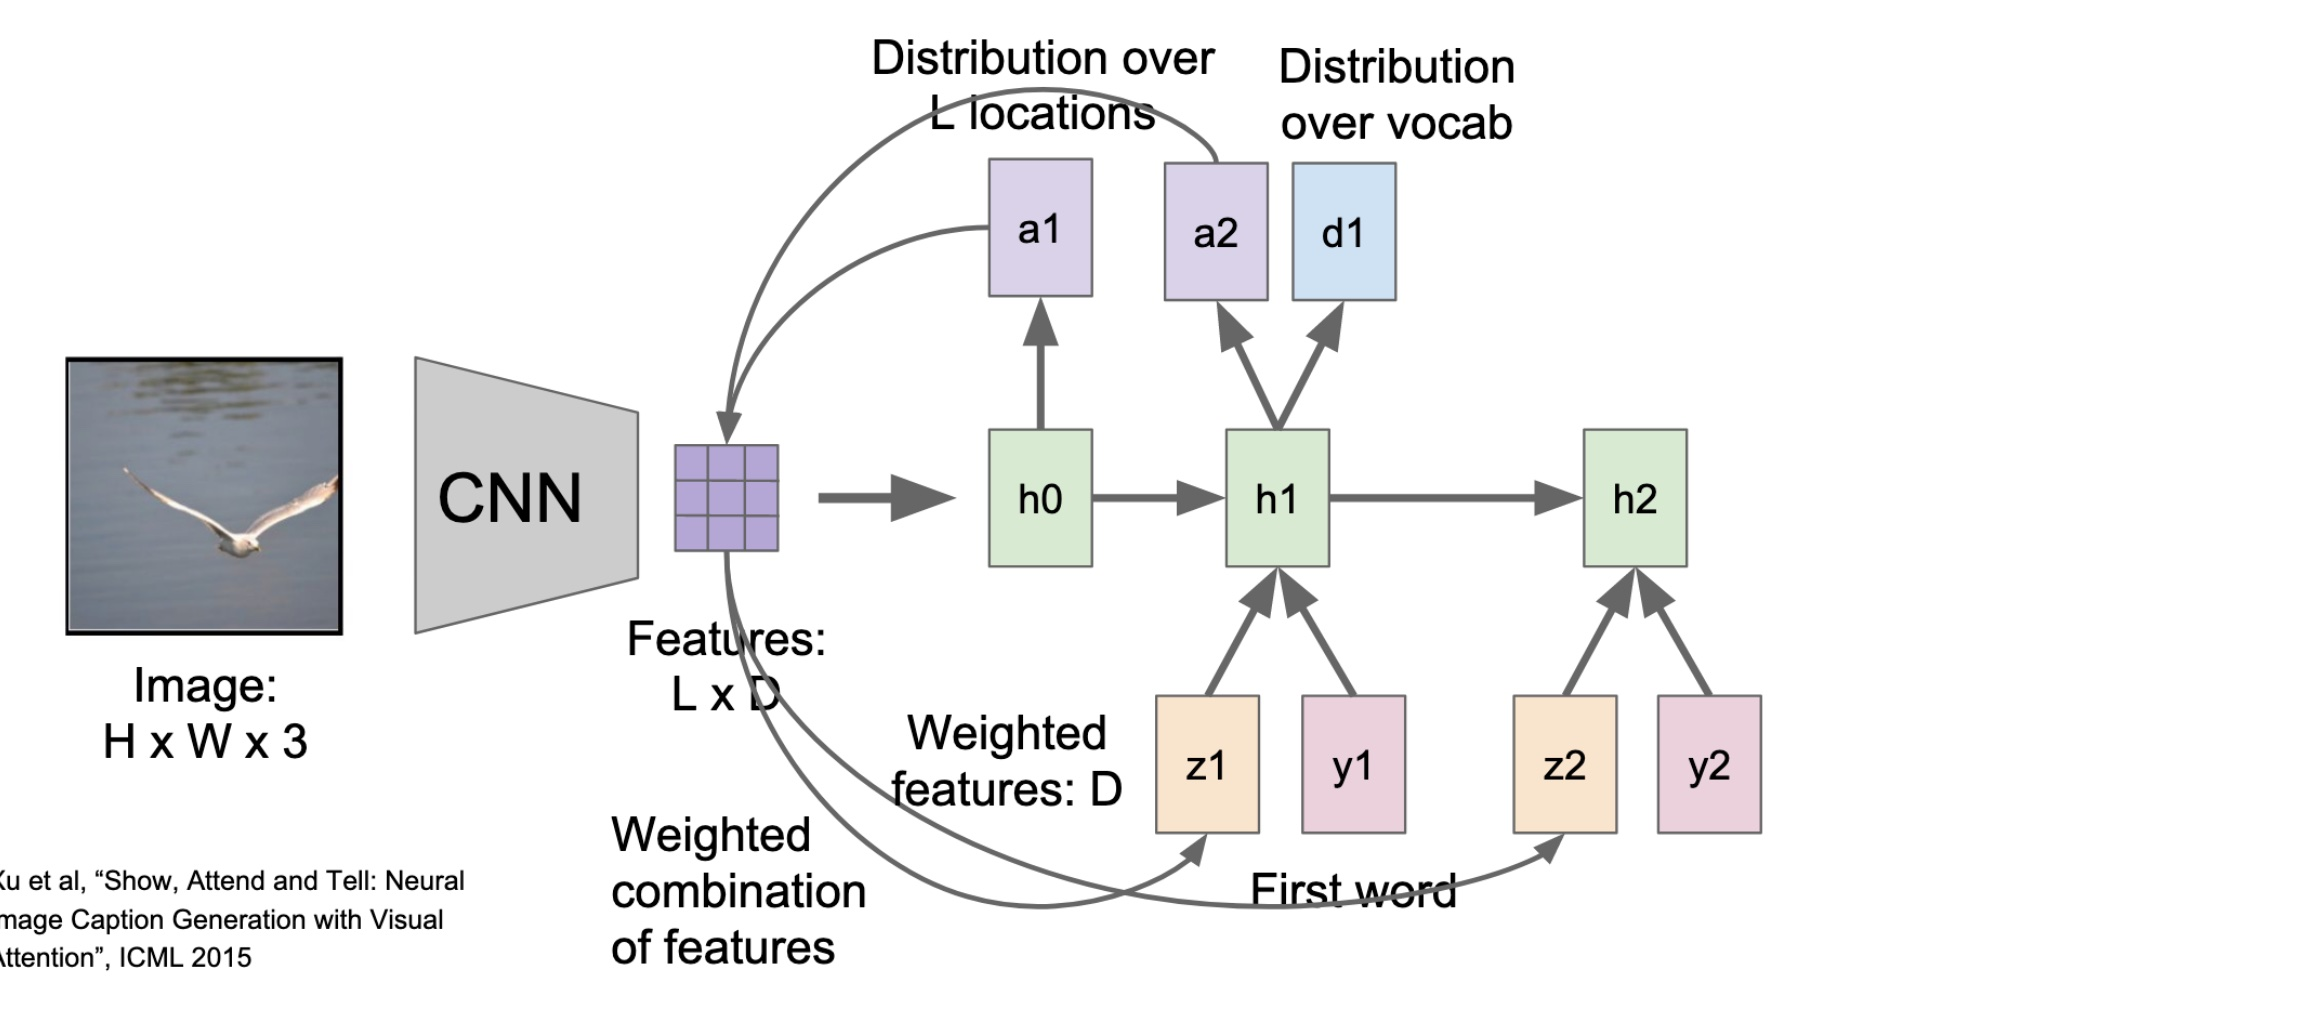
\includegraphics[width=1\textwidth]{pics/att6}
\end{center}
\end{frame}

\begin{frame}
\frametitle{Attention in ICM}
\begin{center}
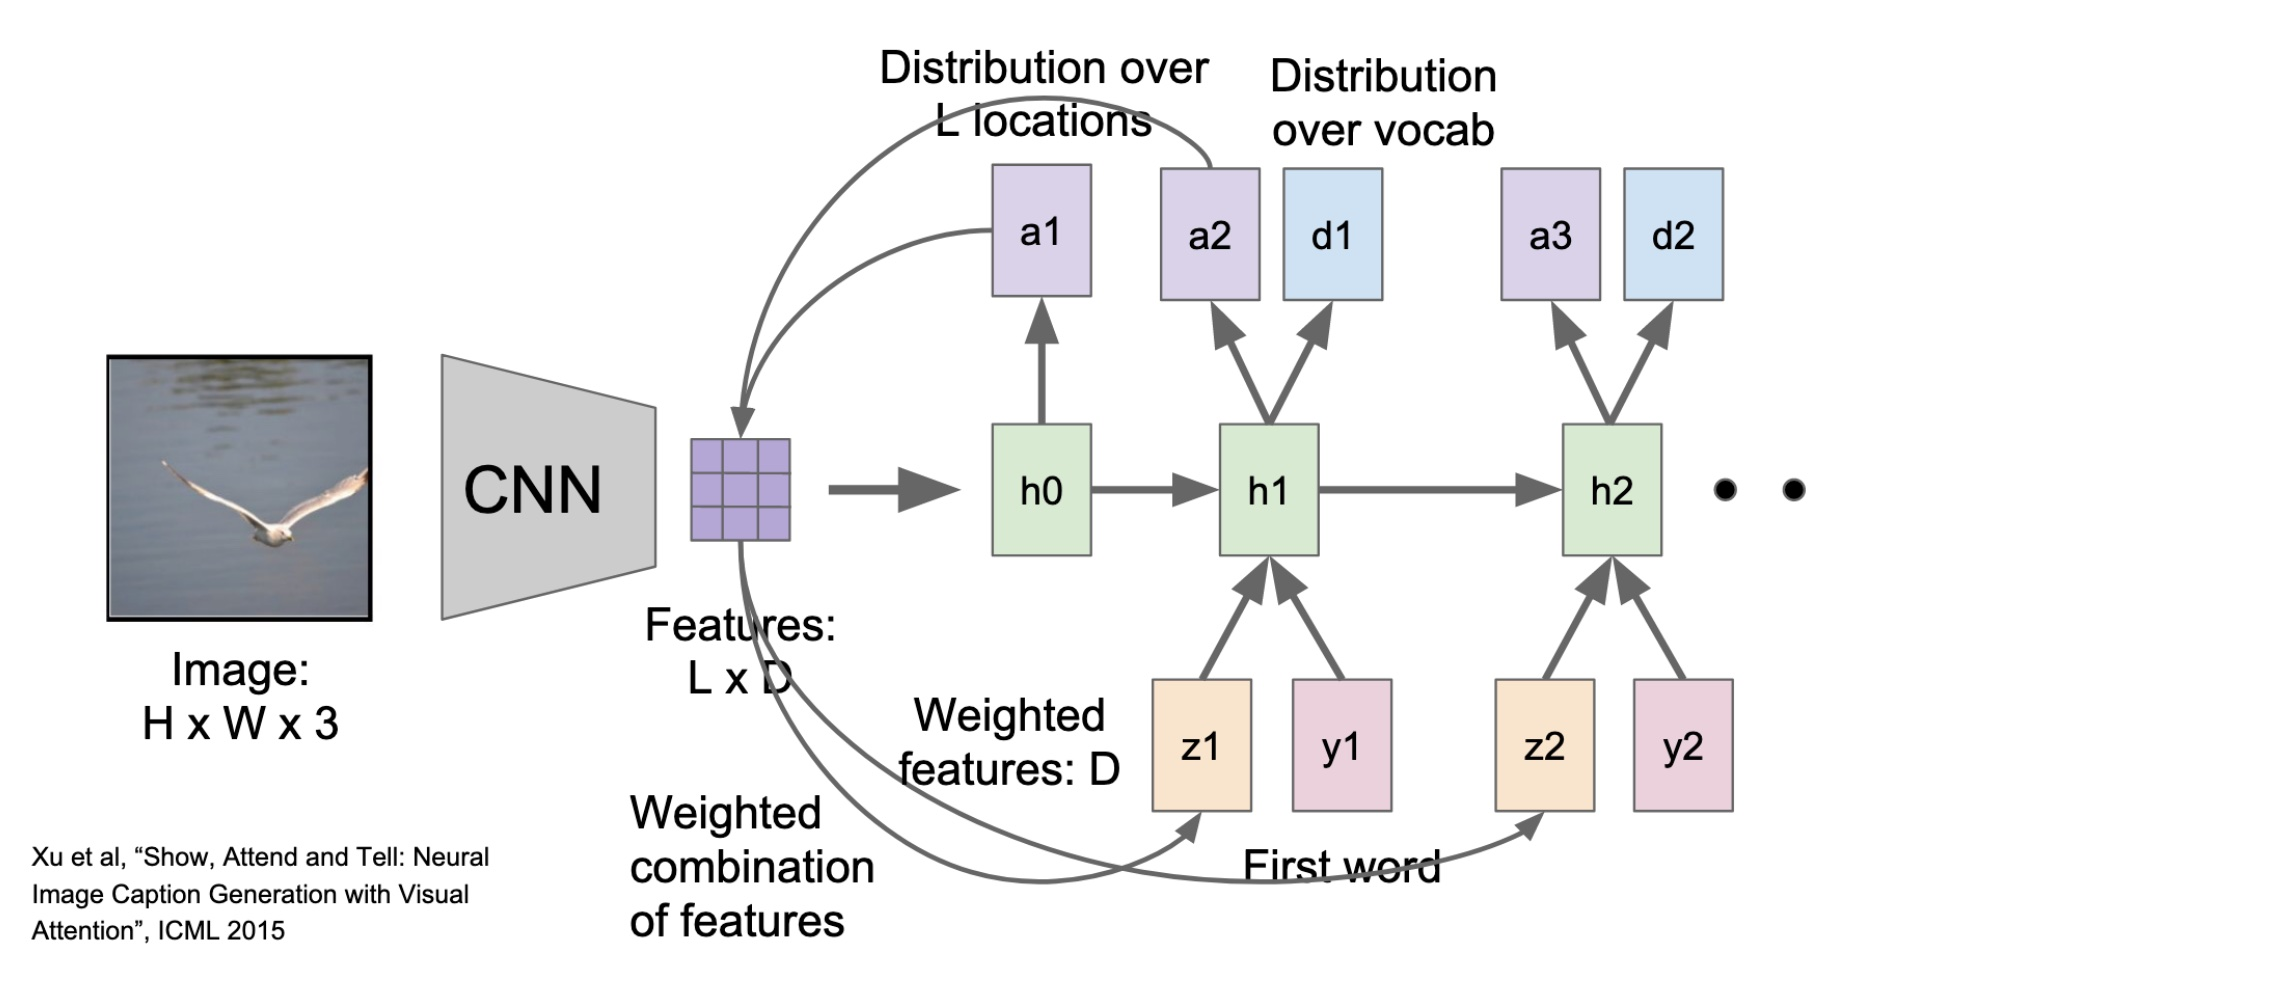
\includegraphics[width=1\textwidth]{pics/att7}
\end{center}
\end{frame}

\begin{frame}
\frametitle{Attention in ICM}
\begin{center}
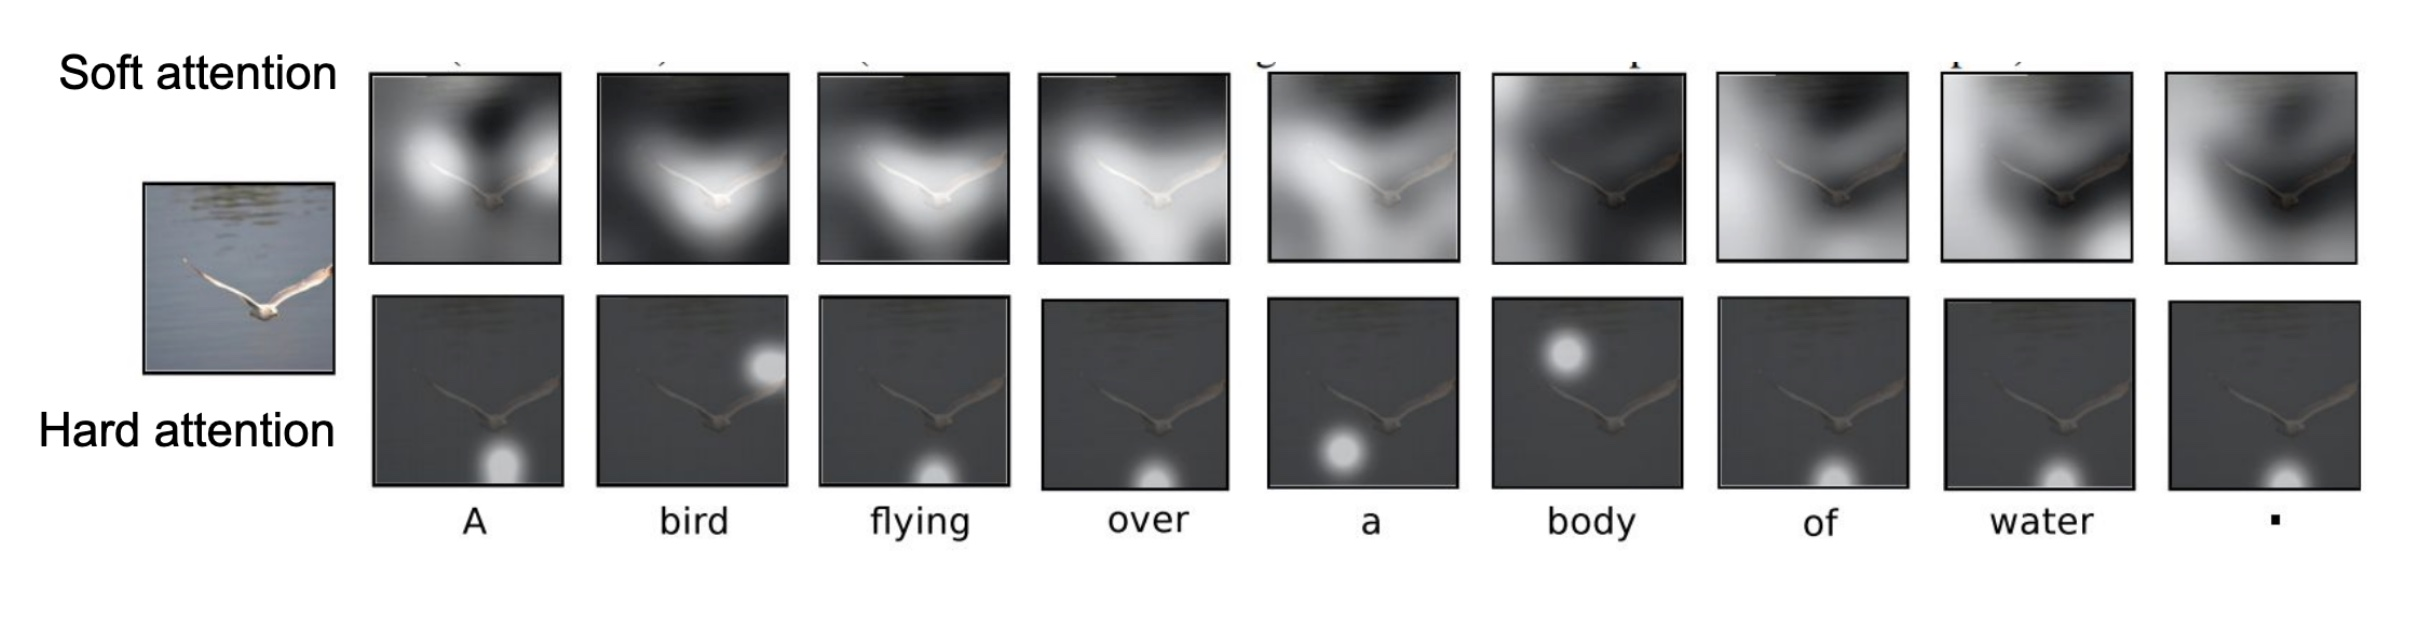
\includegraphics[width=1\textwidth]{pics/att8}
\end{center}
\end{frame}

\begin{frame}
\frametitle{Attention in ICM}
\begin{center}
\includegraphics[width=1\textwidth]{pics/att9}
\end{center}
\end{frame}

\begin{frame}
\frametitle{Attention helps with gender bias in captioning models}
\begin{center}
\includegraphics[width=1\textwidth]{pics/imp1}
\end{center}
\end{frame}

\begin{frame}
\frametitle{Attention helps with dataset biases}
\begin{center}
\includegraphics[width=1\textwidth]{pics/imp2}
\end{center}
\end{frame}

\begin{frame}
\frametitle{Image Captioning Today}
\begin{center}
\includegraphics[width=.95\textwidth]{pics/imp3}
\end{center}
\end{frame}

\begin{frame}
\frametitle{Image Captioning Today}
\begin{center}
\includegraphics[width=.95\textwidth]{pics/imp3}
\end{center}
\end{frame}

\begin{frame}
\frametitle{Conclusions and Future Content}
\begin{itemize}
	\item image captioning is the core task in language-and-vision field
	\pause
	\item standard neural architecture: CNN + LSTM (encoder-decoder, seq-to-seq)
	\pause
	\item SOTA: transformers (all inputs are processed simultaneously)
	\pause
	\item \textit{Next tutorials}: we will look at decoding, evaluation of captioning models, different modes of image representation, more complex tasks (e.g., visual question answering, visual dialogue, situated interaction)
	\pause
	\item \textbf{but now}, we are going to code!
\end{itemize}
\end{frame}


\begin{frame}
\frametitle{Before we start coding...}
\begin{itemize}
	\item An image is worth a thousand words
	\item How to choose the best way to describe an image? And should we even choose one?
\end{itemize}
\end{frame}

\begin{frame}
\frametitle{Before we start coding...}
\begin{itemize}
	\item Each of us describes what we see based on our personal individual background
	\item How do we account for that?
\end{itemize}
\end{frame}

\begin{frame}
\frametitle{Before we start coding...}
\begin{itemize}
	\item What do we want to describe in the image? Which objects are important or not important?
	\pause
	\item When do we want to describe objects? Is there some order of objects that we use?
	\pause
	\item How to describe objects? Which attributes we want to mention and which relations?
\end{itemize}
\end{frame}






%% References

\begin{frame}[allowframebreaks]{References}

\small

% Bibliography

\bibliographystyle{acl_natbib}
\bibliography{bibliography}


\end{frame}





\end{document}


%%% Local Variables:
%%% mode: latex
%%% mode: flyspell
%%% TeX-master: t
%%% TeX-PDF-mode: t
%%% coding: utf-8
%%% ispell-local-dictionary: "british"
%%% End:
